\documentclass[10pt]{article}
\usepackage[T1]{fontenc}
\usepackage{amsmath,amssymb,amsthm}
\usepackage[shortlabels]{enumitem}
\usepackage[english]{babel}
\usepackage[utf8]{inputenc}
\usepackage{fancyhdr}
\usepackage{bold-extra}
\usepackage{color}   
\usepackage{tocloft}
\usepackage{graphicx}
\usepackage{lipsum}
\usepackage{wrapfig}
\usepackage{cutwin}
\usepackage{hyperref}
\usepackage{lastpage}
\usepackage{multicol}
\usepackage{tikz}
\usepackage{float}
\usepackage{algorithm2e}
\usepackage{algorithmic}
\usepackage{chngcntr}

\setcounter{MaxMatrixCols}{20}

% some useful math commands
\newcommand{\eps}{\varepsilon}
\newcommand{\R}{\mathbb{R}}
\newcommand{\C}{\mathbb{C}}
\newcommand{\N}{\mathbb{N}}
\newcommand{\Z}{\mathbb{Z}}
\newcommand{\Q}{\mathbb{Q}}
\newcommand{\K}{\mathbb{K}}
\newcommand{\F}{\mathbb{F}}

\DeclareMathOperator{\ch}{char}
\DeclareMathOperator{\ord}{ord}
\DeclareMathOperator{\GF}{GF}
\DeclareMathOperator{\rank}{rank}
\DeclareMathOperator{\lcm}{lcm}

% title formatting
\newcommand{\newtitle}[4]{
  \begin{center}
	\huge{\textbf{\textsc{#1 Course Notes}}}
    
	\large{\sc #2}
    
	{\sc #3 \textbullet\, #4 \textbullet\, University of Waterloo}
	\normalsize\vspace{1cm}\hrule
  \end{center}
}

% for theorems
\newtheoremstyle{newstyle}      
{} %Aboveskip 
{-0.25pt} %Below skip
{\mdseries} %Body font e.g.\mdseries,\bfseries,\scshape,\itshape
{} %Indent
{\scshape} %Head font e.g.\bfseries,\scshape,\itshape
{.} %Punctuation afer theorem header
{ } %Space after theorem header
{} %Heading

\theoremstyle{newstyle}

\newtheorem*{prop*}{Proposition}
\newtheorem*{cor*}{Corollary}
\newtheorem*{exercise*}{Exercise}
\newtheorem*{lemma*}{Lemma}
\newtheorem*{remark*}{Remark}
\newtheorem*{exmp*}{Example}
\newtheorem*{defn*}{Definition}
\newtheorem*{thm*}{Theorem}
\newtheorem*{notation*}{Notation}
\newtheorem{thm}{Theorem}[subsection]
\newtheorem{fact}[thm]{Fact}
\newtheorem{cor}[thm]{Corollary}
\newtheorem{lemma}[thm]{Lemma}
\newtheorem{remark}[thm]{Remark}
\newtheorem{prop}[thm]{Proposition}
\newtheorem{defn}[thm]{Definition}
\newtheorem{claim}[thm]{Claim}
\newtheorem{axiom}[thm]{Axiom}
\newtheorem{notation}[thm]{Notation}
\newtheorem{exercise}[thm]{Exercise}
\newtheorem{exmp}[thm]{Example}
\newtheorem{algo}[thm]{Algorithm}

% new proof environment
\makeatletter
\newenvironment{pf}[1][\proofname]{\par
  \pushQED{\qed}%
  \normalfont \topsep0\p@\relax
  \trivlist
  \item[\hskip\labelsep\scshape
  #1\@addpunct{.}]\ignorespaces
}{%
  \popQED\endtrivlist\@endpefalse
}
\makeatother

% 1-inch margins
\topmargin 0pt
\advance \topmargin by -\headheight
\advance \topmargin by -\headsep
\textheight 8.9in
\oddsidemargin 0pt
\evensidemargin \oddsidemargin
\marginparwidth 0.5in
\textwidth 6.5in

% \renewcommand{\headrulewidth}{0pt}
% \renewcommand{\footrulewidth}{0.4pt}

\parindent 0in
\parskip 1.5ex

\setlist[itemize]{topsep=0pt}
\setlist[enumerate]{topsep=0pt}

% hyperlinks
\hypersetup{
  colorlinks=true, 
  linktoc=all,     % table of contents is clickable  
  allcolors=black  % all hyperlink colours
}

% table of contents
\addto\captionsenglish{
  \renewcommand{\contentsname}%
    {Table of Contents}%
}
\renewcommand{\cftsecfont}{\normalfont}
\renewcommand{\cftsecpagefont}{\normalfont}
\cftsetindents{section}{0em}{2em}

\fancypagestyle{plain}{%
\fancyhf{} % clear all header and footer fields
\lhead{CO 331: Winter 2021}
\fancyhead[R]{Table of Contents}
%\headrule
\fancyfoot[R]{{\small Page \thepage\ of \pageref*{LastPage}}}
}

% headers and footers
\pagestyle{fancy}
\renewcommand{\sectionmark}[1]{\markboth{#1}{#1}}
\lhead{CO 331: Winter 2021}
\cfoot{}
\setlength\headheight{14pt}

\setcounter{section}{-1}

\begin{document}

\pagestyle{fancy}
\newtitle{CO 331}{Coding Theory}{Alfred Menezes}{Winter 2021}
\rhead{Table of Contents}
\rfoot{{\small Page \thepage\ of \pageref*{LastPage}}}

\tableofcontents
\vspace{1cm}\hrule
\fancyhead[R]{\nouppercase\rightmark}
\newpage 
\fancyhead[R]{Section \thesection: \leftmark}

\section{Introduction}

Coding theory is about clever ways of adding redundancy to messages to allow (efficient) error 
detection and error correction. 

Our basic communications model which we will use throughout the course is as follows.

\tikzset{every picture/.style={line width=0.75pt}} %set default line width to 0.75pt        

\begin{center}
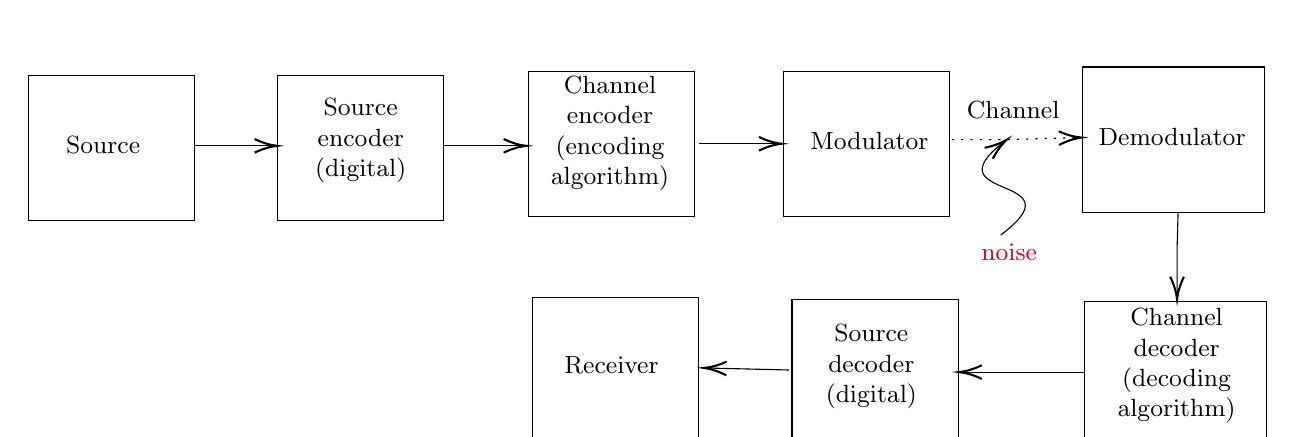
\begin{tikzpicture}[x=0.75pt,y=0.75pt,yscale=-1,xscale=1]
%uncomment if require: \path (0,225); %set diagram left start at 0, and has height of 225

%Straight Lines [id:da23834982365428936] 
\draw    (110,64) -- (136.5,64) -- (148,64) ;
\draw [shift={(150,64)}, rotate = 180] [color={rgb, 255:red, 0; green, 0; blue, 0 }  ][line width=0.75]    (10.93,-3.29) .. controls (6.95,-1.4) and (3.31,-0.3) .. (0,0) .. controls (3.31,0.3) and (6.95,1.4) .. (10.93,3.29)   ;
%Flowchart: Process [id:dp9909741212346586] 
\draw   (30,30) -- (110,30) -- (110,100) -- (30,100) -- cycle ;
%Flowchart: Process [id:dp2697977096239874] 
\draw   (150,30) -- (230,30) -- (230,100) -- (150,100) -- cycle ;
%Flowchart: Process [id:dp9249849749328085] 
\draw   (271,28) -- (351,28) -- (351,98) -- (271,98) -- cycle ;
%Straight Lines [id:da11362394248007979] 
\draw    (230,64) -- (256.5,64) -- (268,64) ;
\draw [shift={(270,64)}, rotate = 180] [color={rgb, 255:red, 0; green, 0; blue, 0 }  ][line width=0.75]    (10.93,-3.29) .. controls (6.95,-1.4) and (3.31,-0.3) .. (0,0) .. controls (3.31,0.3) and (6.95,1.4) .. (10.93,3.29)   ;
%Straight Lines [id:da6864496627109067] 
\draw    (353,63) -- (379.5,63) -- (391,63) ;
\draw [shift={(393,63)}, rotate = 180] [color={rgb, 255:red, 0; green, 0; blue, 0 }  ][line width=0.75]    (10.93,-3.29) .. controls (6.95,-1.4) and (3.31,-0.3) .. (0,0) .. controls (3.31,0.3) and (6.95,1.4) .. (10.93,3.29)   ;
%Flowchart: Process [id:dp300918507367262] 
\draw   (394,28) -- (474,28) -- (474,98) -- (394,98) -- cycle ;
%Straight Lines [id:da4887614634526103] 
\draw  [dash pattern={on 0.84pt off 2.51pt}]  (475,61) -- (501.5,61) -- (535.5,60.06) ;
\draw [shift={(537.5,60)}, rotate = 538.4100000000001] [color={rgb, 255:red, 0; green, 0; blue, 0 }  ][line width=0.75]    (10.93,-3.29) .. controls (6.95,-1.4) and (3.31,-0.3) .. (0,0) .. controls (3.31,0.3) and (6.95,1.4) .. (10.93,3.29)   ;
%Curve Lines [id:da5549987538694752] 
\draw    (498.5,107) .. controls (538.1,77.3) and (463.03,90.72) .. (500.33,61.89) ;
\draw [shift={(501.5,61)}, rotate = 503.13] [color={rgb, 255:red, 0; green, 0; blue, 0 }  ][line width=0.75]    (10.93,-3.29) .. controls (6.95,-1.4) and (3.31,-0.3) .. (0,0) .. controls (3.31,0.3) and (6.95,1.4) .. (10.93,3.29)   ;
%Flowchart: Process [id:dp13427120496160616] 
\draw   (538,26) -- (625.5,26) -- (625.5,96) -- (538,96) -- cycle ;
%Straight Lines [id:da8442705350817545] 
\draw    (584,96) -- (583.5,114) -- (583.5,136) ;
\draw [shift={(583.5,138)}, rotate = 270] [color={rgb, 255:red, 0; green, 0; blue, 0 }  ][line width=0.75]    (10.93,-3.29) .. controls (6.95,-1.4) and (3.31,-0.3) .. (0,0) .. controls (3.31,0.3) and (6.95,1.4) .. (10.93,3.29)   ;
%Flowchart: Process [id:dp8353125777110129] 
\draw   (539,139) -- (626.5,139) -- (626.5,209) -- (539,209) -- cycle ;
%Straight Lines [id:da03051329752100651] 
\draw    (538.5,173) -- (480.5,173) ;
\draw [shift={(478.5,173)}, rotate = 360] [color={rgb, 255:red, 0; green, 0; blue, 0 }  ][line width=0.75]    (10.93,-3.29) .. controls (6.95,-1.4) and (3.31,-0.3) .. (0,0) .. controls (3.31,0.3) and (6.95,1.4) .. (10.93,3.29)   ;
%Flowchart: Process [id:dp2819678670933694] 
\draw   (398,138) -- (478,138) -- (478,208) -- (398,208) -- cycle ;
%Straight Lines [id:da6275131518556043] 
\draw    (396.5,172) -- (357.5,171.05) ;
\draw [shift={(355.5,171)}, rotate = 361.4] [color={rgb, 255:red, 0; green, 0; blue, 0 }  ][line width=0.75]    (10.93,-3.29) .. controls (6.95,-1.4) and (3.31,-0.3) .. (0,0) .. controls (3.31,0.3) and (6.95,1.4) .. (10.93,3.29)   ;
%Flowchart: Process [id:dp4201838841011669] 
\draw   (273,137) -- (353,137) -- (353,207) -- (273,207) -- cycle ;

% Text Node
\draw (47,58) node [anchor=north west][inner sep=0.75pt]  [font=\small] [align=left] {Source};
% Text Node
\draw (165,40) node [anchor=north west][inner sep=0.75pt]  [font=\small] [align=left] {\begin{minipage}[lt]{35.901892000000004pt}\setlength\topsep{0pt}
\begin{center}
Source\\encoder\\(digital)
\end{center}

\end{minipage}};
% Text Node
\draw (280,29) node [anchor=north west][inner sep=0.75pt]  [font=\small] [align=left] {\begin{minipage}[lt]{43.541216pt}\setlength\topsep{0pt}
\begin{center}
Channel\\encoder\\(encoding\\algorithm)
\end{center}

\end{minipage}};
% Text Node
\draw (405,56) node [anchor=north west][inner sep=0.75pt]  [font=\small] [align=left] {\begin{minipage}[lt]{43.551892pt}\setlength\topsep{0pt}
\begin{center}
Modulator
\end{center}

\end{minipage}};
% Text Node
\draw (481,41) node [anchor=north west][inner sep=0.75pt]  [font=\small] [align=left] {{\small Channe}l};
% Text Node
\draw (488,110) node [anchor=north west][inner sep=0.75pt]  [font=\small] [align=left] {\textcolor[rgb]{0.82,0.01,0.11}{noise}};
% Text Node
\draw (543,54) node [anchor=north west][inner sep=0.75pt]  [font=\small] [align=left] {\begin{minipage}[lt]{55.281892pt}\setlength\topsep{0pt}
\begin{center}
Demodulator
\end{center}

\end{minipage}};
% Text Node
\draw (553,141) node [anchor=north west][inner sep=0.75pt]  [font=\small] [align=left] {\begin{minipage}[lt]{43.541216pt}\setlength\topsep{0pt}
\begin{center}
Channel\\decoder\\(decoding\\algorithm)
\end{center}

\end{minipage}};
% Text Node
\draw (411,149) node [anchor=north west][inner sep=0.75pt]  [font=\small] [align=left] {\begin{minipage}[lt]{35.901892000000004pt}\setlength\topsep{0pt}
\begin{center}
Source\\decoder\\(digital)
\end{center}

\end{minipage}};
% Text Node
\draw (287,164) node [anchor=north west][inner sep=0.75pt]  [font=\small] [align=left] {Receiver};

\end{tikzpicture}
\end{center}

Below, we give some examples of codes.

{\bf Parity code.}
\begin{itemize}
    \item {\bf Encoding algorithm:} Add a $0$ bit to the (binary) message $m$ if the number of 
    $1$'s in $m$ is even; else add a $1$ bit.
    \item {\bf Decoding algorithm:} If the number of $1$'s in a received message $r$ is even, 
    then accept $r$; else declare that an error has occurred.
\end{itemize}
We note that if no errors occur during transmission of a message $r$, then the decoding 
algorithm will correctly accept $r$. Indeed, if the number of bits flipped is odd, then 
the parity of $r$ is odd, and so the channel decoder will correctly declare that 
at least one error has occurred. On the other hand, if the number of bits flipped 
is even, then the parity of $r$ is even, and hence the decoder correctly accepts $r$.

{\bf Replication code.} For error correction, we are using "nearest neighbour decoding".
\begin{table}[h]
\centering
\begin{tabular}{|c|c|c|c|c|}
\hline
\begin{tabular}[c]{@{}c@{}}Source\\ messages\end{tabular} & Codeword                                                  & \begin{tabular}[c]{@{}c@{}}Number of errors\\ per codeword that\\ can always be detected\end{tabular} & \begin{tabular}[c]{@{}c@{}}Number of errors\\ per codeword that\\ can always be corrected \end{tabular} & \begin{tabular}[c]{@{}c@{}}Information\\ rate\end{tabular} \\ \hline
\begin{tabular}[c]{@{}c@{}}$0$\\ $1$\end{tabular}         & \begin{tabular}[c]{@{}c@{}}$0$\\ $1$\end{tabular}         & $0$                                                                                                   & $0$                                                                                                              & $1$                                                        \\ \hline
\begin{tabular}[c]{@{}c@{}}$0$\\ $1$\end{tabular}         & \begin{tabular}[c]{@{}c@{}}$00$\\ $11$\end{tabular}       & $1$                                                                                                   & $0$                                                                                                              & $1/2$                                                      \\ \hline
\begin{tabular}[c]{@{}c@{}}$0$\\ $1$\end{tabular}         & \begin{tabular}[c]{@{}c@{}}$000$\\ $111$\end{tabular}     & $2$                                                                                                   & $1$                                                                                                              & $1/3$                                                      \\ \hline
\begin{tabular}[c]{@{}c@{}}$0$\\ $1$\end{tabular}         & \begin{tabular}[c]{@{}c@{}}$0000$\\ $1111$\end{tabular}   & $3$                                                                                                   & $1$                                                                                                              & $1/4$                                                      \\ \hline
\begin{tabular}[c]{@{}c@{}}$0$\\ $1$\end{tabular}         & \begin{tabular}[c]{@{}c@{}}$00000$\\ $11111$\end{tabular} & $4$                                                                                                   & $2$                                                                                                              & $1/5$                                                      \\ \hline
\end{tabular}
\end{table}

We see that we can always increase the error detecting capability and also the error correcting 
capability by increasing the number of times a bit is replicated. However, the price to 
pay for this is a decreasing information rate. This is a waste of potentially expensive bandwidth.

{\bf Goals of coding theory.} We wish to design codes such that
\begin{enumerate}[(i)]
    \item the error-correcting capability is high;
    \item the information rate is high; and
    \item encoding and decoding can be done efficiently.
\end{enumerate}

{\bf Course overview.} The course will deal with algebraic methods of designing good 
(block) codes. The focus is on error correction, not error detection. These codes are used 
in wireless communications, space probes, CD/DVD players, storage, QR codes, and more. 

{\bf Not covered in the course.} Modern families of codes such as Turbo codes, LDPC codes, and Raptor
codes due to lack of time, and the math used is not as elegant as the ones covered in the course.

{\bf The big picture.} Coding theory in its broadest sense deals with techniques for the 
{\bf efficient}, {\bf secure}, and {\bf reliable} transmission of data over communication channels 
that may be subject to {\bf non-malicious errors} (noise) and {\bf adversarial intrusion}. 
The latter includes passive intrusion (eavesdropping) and active intrusion (injection, 
deletion, modification).

Efficiency is associated with data compression, security is associated with cryptography, 
and reliability is associated with error correcting codes. They fit into our 
basic communications as shown in the diagram below.

\tikzset{every picture/.style={line width=0.75pt}} %set default line width to 0.75pt        

\begin{center}
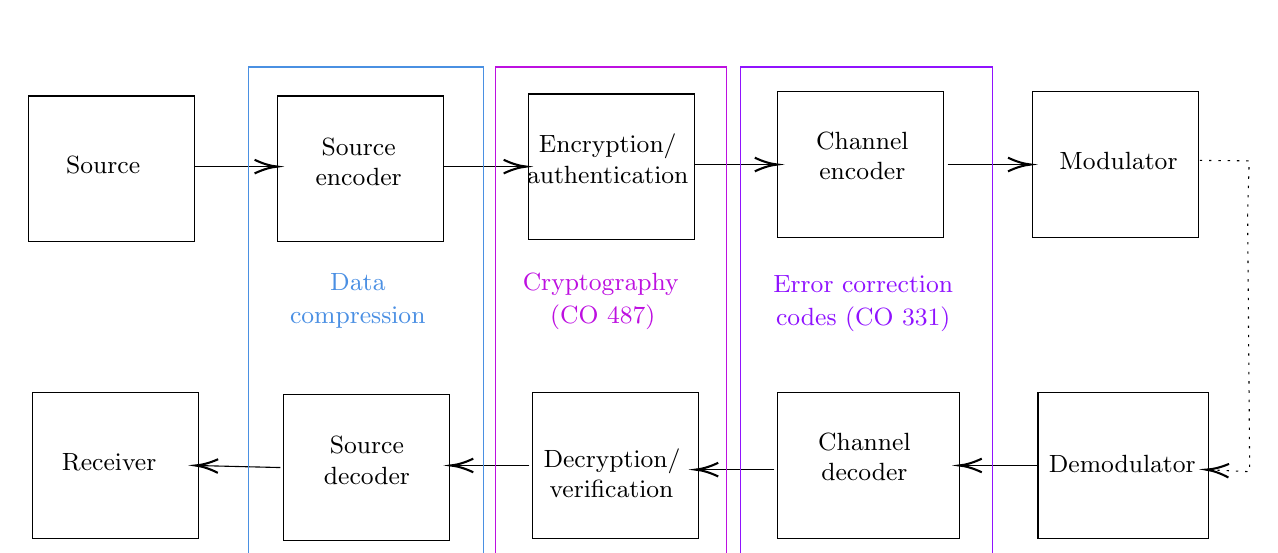
\begin{tikzpicture}[x=0.75pt,y=0.75pt,yscale=-1,xscale=1]
%uncomment if require: \path (0,438); %set diagram left start at 0, and has height of 438

%Straight Lines [id:da23834982365428936] 
\draw    (110,64) -- (136.5,64) -- (148,64) ;
\draw [shift={(150,64)}, rotate = 180] [color={rgb, 255:red, 0; green, 0; blue, 0 }  ][line width=0.75]    (10.93,-3.29) .. controls (6.95,-1.4) and (3.31,-0.3) .. (0,0) .. controls (3.31,0.3) and (6.95,1.4) .. (10.93,3.29)   ;
%Flowchart: Process [id:dp9909741212346586] 
\draw   (30,30) -- (110,30) -- (110,100) -- (30,100) -- cycle ;
%Flowchart: Process [id:dp2697977096239874] 
\draw   (150,30) -- (230,30) -- (230,100) -- (150,100) -- cycle ;
%Flowchart: Process [id:dp9249849749328085] 
\draw   (391,28) -- (471,28) -- (471,98) -- (391,98) -- cycle ;
%Straight Lines [id:da11362394248007979] 
\draw    (230,64) -- (256.5,64) -- (268,64) ;
\draw [shift={(270,64)}, rotate = 180] [color={rgb, 255:red, 0; green, 0; blue, 0 }  ][line width=0.75]    (10.93,-3.29) .. controls (6.95,-1.4) and (3.31,-0.3) .. (0,0) .. controls (3.31,0.3) and (6.95,1.4) .. (10.93,3.29)   ;
%Straight Lines [id:da6864496627109067] 
\draw    (473,63) -- (499.5,63) -- (511,63) ;
\draw [shift={(513,63)}, rotate = 180] [color={rgb, 255:red, 0; green, 0; blue, 0 }  ][line width=0.75]    (10.93,-3.29) .. controls (6.95,-1.4) and (3.31,-0.3) .. (0,0) .. controls (3.31,0.3) and (6.95,1.4) .. (10.93,3.29)   ;
%Flowchart: Process [id:dp300918507367262] 
\draw   (514,28) -- (594,28) -- (594,98) -- (514,98) -- cycle ;
%Straight Lines [id:da4887614634526103] 
\draw  [dash pattern={on 0.84pt off 2.51pt}]  (617.5,87) -- (618.5,211) -- (599.5,210.1) ;
\draw [shift={(597.5,210)}, rotate = 362.73] [color={rgb, 255:red, 0; green, 0; blue, 0 }  ][line width=0.75]    (10.93,-3.29) .. controls (6.95,-1.4) and (3.31,-0.3) .. (0,0) .. controls (3.31,0.3) and (6.95,1.4) .. (10.93,3.29)   ;
%Flowchart: Process [id:dp13427120496160616] 
\draw   (516.5,173) -- (598.5,173) -- (598.5,243) -- (516.5,243) -- cycle ;
%Straight Lines [id:da03051329752100651] 
\draw    (271.5,208) -- (235.5,208) ;
\draw [shift={(233.5,208)}, rotate = 360] [color={rgb, 255:red, 0; green, 0; blue, 0 }  ][line width=0.75]    (10.93,-3.29) .. controls (6.95,-1.4) and (3.31,-0.3) .. (0,0) .. controls (3.31,0.3) and (6.95,1.4) .. (10.93,3.29)   ;
%Flowchart: Process [id:dp2819678670933694] 
\draw   (153,174) -- (233,174) -- (233,244) -- (153,244) -- cycle ;
%Straight Lines [id:da6275131518556043] 
\draw    (151.5,209) -- (112.5,208.05) ;
\draw [shift={(110.5,208)}, rotate = 361.4] [color={rgb, 255:red, 0; green, 0; blue, 0 }  ][line width=0.75]    (10.93,-3.29) .. controls (6.95,-1.4) and (3.31,-0.3) .. (0,0) .. controls (3.31,0.3) and (6.95,1.4) .. (10.93,3.29)   ;
%Flowchart: Process [id:dp4201838841011669] 
\draw   (32,173) -- (112,173) -- (112,243) -- (32,243) -- cycle ;
%Straight Lines [id:da6139762451819093] 
\draw  [dash pattern={on 0.84pt off 2.51pt}]  (594.5,61) -- (618.25,61.25) -- (617.5,87) ;
%Flowchart: Process [id:dp3118980477214841] 
\draw   (271,29) -- (351,29) -- (351,99) -- (271,99) -- cycle ;
%Straight Lines [id:da5034263589182224] 
\draw    (351,63) -- (377.5,63) -- (389,63) ;
\draw [shift={(391,63)}, rotate = 180] [color={rgb, 255:red, 0; green, 0; blue, 0 }  ][line width=0.75]    (10.93,-3.29) .. controls (6.95,-1.4) and (3.31,-0.3) .. (0,0) .. controls (3.31,0.3) and (6.95,1.4) .. (10.93,3.29)   ;
%Flowchart: Process [id:dp44899663049808103] 
\draw   (273,173) -- (353,173) -- (353,243) -- (273,243) -- cycle ;
%Flowchart: Process [id:dp9506862221454981] 
\draw   (391,173) -- (478.5,173) -- (478.5,243) -- (391,243) -- cycle ;
%Straight Lines [id:da6533335792478188] 
\draw    (389.5,210) -- (353.5,210) ;
\draw [shift={(351.5,210)}, rotate = 360] [color={rgb, 255:red, 0; green, 0; blue, 0 }  ][line width=0.75]    (10.93,-3.29) .. controls (6.95,-1.4) and (3.31,-0.3) .. (0,0) .. controls (3.31,0.3) and (6.95,1.4) .. (10.93,3.29)   ;
%Straight Lines [id:da776221405009176] 
\draw    (516.5,208) -- (480.5,208) ;
\draw [shift={(478.5,208)}, rotate = 360] [color={rgb, 255:red, 0; green, 0; blue, 0 }  ][line width=0.75]    (10.93,-3.29) .. controls (6.95,-1.4) and (3.31,-0.3) .. (0,0) .. controls (3.31,0.3) and (6.95,1.4) .. (10.93,3.29)   ;
%Flowchart: Process [id:dp701134048177743] 
\draw  [color={rgb, 255:red, 74; green, 144; blue, 226 }  ,draw opacity=1 ] (136,16) -- (249.5,16) -- (249.5,255) -- (136,255) -- cycle ;
%Flowchart: Process [id:dp7749552458781244] 
\draw  [color={rgb, 255:red, 144; green, 19; blue, 254 }  ,draw opacity=1 ] (373,16) -- (494.5,16) -- (494.5,251) -- (373,251) -- cycle ;
%Flowchart: Process [id:dp9162174967039207] 
\draw  [color={rgb, 255:red, 189; green, 16; blue, 224 }  ,draw opacity=1 ] (255,16) -- (366.5,16) -- (366.5,253) -- (255,253) -- cycle ;

% Text Node
\draw (47,58) node [anchor=north west][inner sep=0.75pt]  [font=\small] [align=left] {Source};
% Text Node
\draw (164,49) node [anchor=north west][inner sep=0.75pt]  [font=\small] [align=left] {\begin{minipage}[lt]{35.901892000000004pt}\setlength\topsep{0pt}
\begin{center}
Source\\encoder
\end{center}

\end{minipage}};
% Text Node
\draw (406,46) node [anchor=north west][inner sep=0.75pt]  [font=\small] [align=left] {\begin{minipage}[lt]{36.921892pt}\setlength\topsep{0pt}
\begin{center}
Channel\\encoder
\end{center}

\end{minipage}};
% Text Node
\draw (525,56) node [anchor=north west][inner sep=0.75pt]  [font=\small] [align=left] {\begin{minipage}[lt]{43.551892pt}\setlength\topsep{0pt}
\begin{center}
Modulator
\end{center}

\end{minipage}};
% Text Node
\draw (519,202) node [anchor=north west][inner sep=0.75pt]  [font=\small] [align=left] {\begin{minipage}[lt]{55.281892pt}\setlength\topsep{0pt}
\begin{center}
Demodulator
\end{center}

\end{minipage}};
% Text Node
\draw (168,193) node [anchor=north west][inner sep=0.75pt]  [font=\small] [align=left] {\begin{minipage}[lt]{35.901892000000004pt}\setlength\topsep{0pt}
\begin{center}
Source\\decoder
\end{center}

\end{minipage}};
% Text Node
\draw (45,201) node [anchor=north west][inner sep=0.75pt]  [font=\small] [align=left] {Receiver};
% Text Node
\draw (268,47) node [anchor=north west][inner sep=0.75pt]  [font=\small] [align=left] {\begin{minipage}[lt]{59.893108000000005pt}\setlength\topsep{0pt}
\begin{center}
Encryption/\\authentication
\end{center}

\end{minipage}};
% Text Node
\draw (277,193) node [anchor=north west][inner sep=0.75pt]  [font=\small] [align=left] {\begin{minipage}[lt]{49.151216000000005pt}\setlength\topsep{0pt}
\begin{center}
Decryption/\\verification
\end{center}

\end{minipage}};
% Text Node
\draw (407,191) node [anchor=north west][inner sep=0.75pt]  [font=\small] [align=left] {\begin{minipage}[lt]{36.921892pt}\setlength\topsep{0pt}
\begin{center}
Channel\\decoder
\end{center}

\end{minipage}};
% Text Node
\draw (151,114) node [anchor=north west][inner sep=0.75pt]   [align=left] {\begin{minipage}[lt]{54.761216000000005pt}\setlength\topsep{0pt}
\begin{center}
\textcolor[rgb]{0.29,0.56,0.89}{{\small Data}}\\\textcolor[rgb]{0.29,0.56,0.89}{{\small compression}}
\end{center}

\end{minipage}};
% Text Node
\draw (267,114) node [anchor=north west][inner sep=0.75pt]   [align=left] {\begin{minipage}[lt]{57.831892pt}\setlength\topsep{0pt}
{\small \textcolor[rgb]{0.74,0.06,0.88}{Cryptography}}
\begin{center}
{\small \textcolor[rgb]{0.74,0.06,0.88}{(CO 487)}}
\end{center}

\end{minipage}};
% Text Node
\draw (386,115) node [anchor=north west][inner sep=0.75pt]   [align=left] {\begin{minipage}[lt]{67.521892pt}\setlength\topsep{0pt}
\begin{center}
{\small \textcolor[rgb]{0.56,0.07,1}{Error correction}}\\{\small \textcolor[rgb]{0.56,0.07,1}{codes (CO 331)}}
\end{center}

\end{minipage}};

\end{tikzpicture}
\end{center}

\newpage 
\section{Fundamentals}

\subsection{Basic definitions and concepts}

\begin{defn}~
\begin{itemize}
    \item An {\bf alphabet} is a finite set of $q \geq 2$ symbols.
    \item A {\bf word} (also known as a {\bf vector} or {\bf tuple}) 
    is a finite sequence of symbols from $A$.
    \item A {\bf code} $C$ over $A$ is a set of words of size at least $2$.
    \item A {\bf codeword} is a word in the code $C$.
    \item A {\bf block code} is a code in which all codewords have the same length.
    \item A {\bf block code of length $n$ containing $M$ codewords over $A$} is a 
    subset $C \subseteq A^n$ with $|C| = M$. We call $C$ an {\bf $[n, M]$-code} over $A$.
\end{itemize}
\end{defn}

\begin{exmp}
The code $C = \{00000, 11100, 00111, 10101\}$ is a $[5, 4]$-code over $\{0, 1\}$. The following 
is an encoding of messages (an injective function).

\begin{center}
\tikzset{every picture/.style={line width=0.75pt}} %set default line width to 0.75pt        

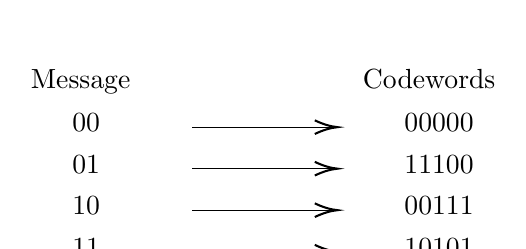
\begin{tikzpicture}[x=0.75pt,y=0.75pt,yscale=-1,xscale=1]
%uncomment if require: \path (0,438); %set diagram left start at 0, and has height of 438

%Straight Lines [id:da8724810404041419] 
\draw    (190,100) -- (258,100) ;
\draw [shift={(260,100)}, rotate = 180] [color={rgb, 255:red, 0; green, 0; blue, 0 }  ][line width=0.75]    (10.93,-3.29) .. controls (6.95,-1.4) and (3.31,-0.3) .. (0,0) .. controls (3.31,0.3) and (6.95,1.4) .. (10.93,3.29)   ;
%Straight Lines [id:da03521599146141208] 
\draw    (190,120) -- (258,120) ;
\draw [shift={(260,120)}, rotate = 180] [color={rgb, 255:red, 0; green, 0; blue, 0 }  ][line width=0.75]    (10.93,-3.29) .. controls (6.95,-1.4) and (3.31,-0.3) .. (0,0) .. controls (3.31,0.3) and (6.95,1.4) .. (10.93,3.29)   ;
%Straight Lines [id:da7424467118479079] 
\draw    (190,140) -- (258,140) ;
\draw [shift={(260,140)}, rotate = 180] [color={rgb, 255:red, 0; green, 0; blue, 0 }  ][line width=0.75]    (10.93,-3.29) .. controls (6.95,-1.4) and (3.31,-0.3) .. (0,0) .. controls (3.31,0.3) and (6.95,1.4) .. (10.93,3.29)   ;
%Straight Lines [id:da9422028159912972] 
\draw    (190,160) -- (258,160) ;
\draw [shift={(260,160)}, rotate = 180] [color={rgb, 255:red, 0; green, 0; blue, 0 }  ][line width=0.75]    (10.93,-3.29) .. controls (6.95,-1.4) and (3.31,-0.3) .. (0,0) .. controls (3.31,0.3) and (6.95,1.4) .. (10.93,3.29)   ;

% Text Node
\draw (111,71) node [anchor=north west][inner sep=0.75pt]   [align=left] {Message};
% Text Node
\draw (271,71) node [anchor=north west][inner sep=0.75pt]   [align=left] {Codewords};
% Text Node
\draw (131,92.4) node [anchor=north west][inner sep=0.75pt]    {$00$};
% Text Node
\draw (131,112.4) node [anchor=north west][inner sep=0.75pt]    {$01$};
% Text Node
\draw (291,92.4) node [anchor=north west][inner sep=0.75pt]    {$00000$};
% Text Node
\draw (291,112.4) node [anchor=north west][inner sep=0.75pt]    {$11100$};
% Text Node
\draw (131,132.4) node [anchor=north west][inner sep=0.75pt]    {$10$};
% Text Node
\draw (131,152.4) node [anchor=north west][inner sep=0.75pt]    {$11$};
% Text Node
\draw (291,132.4) node [anchor=north west][inner sep=0.75pt]    {$00111$};
% Text Node
\draw (291,152.4) node [anchor=north west][inner sep=0.75pt]    {$10101$};
\end{tikzpicture}
\end{center}
\end{exmp}

The channel encoder only transmits codewords. However, what is received may not be a codeword. 
For instance, suppose $r = 11000$ is received in Example 1.1.2. What should the channel decoder do? 

Before we can answer this question, we should make some assumptions about the channel 
which we will use throughout the course. These will help determine whether a decoding strategy 
is good or not.

{\bf Assumptions about the channel.} 
\begin{enumerate}[(1)]
    \item The channel transmits only symbols from $A$ ("hard decision decoding").
    \item No symbols are lost, added, or interchanged during transmission. 
    (In practice, this may happen, but this can be accounted for using various techniques 
    which we will not cover in this course.)
    \item The channel is a {\bf $q$-symmetric channel}. That is, if
    $A = \{a_1, \dots, a_q\}$, $X_i$ denotes the $i$-th symbol sent, and 
    $Y_i$ denotes the $i$-th symbol received, then for all $i \geq 1$ and 
    $1 \leq j, k \leq q$, we have 
    \[ P(Y_i = a_j \mid X_i = a_k) = \begin{cases} 1-p & \text{if } j=k \\ 
    \frac{p}{q-1} & \text{if } j\neq k. \end{cases} \]
    We call $p$ the {\bf symbol error probability} of the channel (we have $0 \leq p \leq 1$).
\end{enumerate}

\begin{defn}
A $2$-symmetric channel is called a {\bf binary symmetric channel (BSC)}.
\end{defn}

\tikzset{every picture/.style={line width=0.75pt}} %set default line width to 0.75pt        
\begin{center}
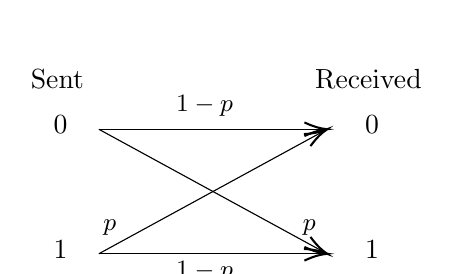
\begin{tikzpicture}[x=0.75pt,y=0.75pt,yscale=-1,xscale=1]
%uncomment if require: \path (0,438); %set diagram left start at 0, and has height of 438

%Straight Lines [id:da8724810404041419] 
\draw    (170,100) -- (278,100) ;
\draw [shift={(280,100)}, rotate = 180] [color={rgb, 255:red, 0; green, 0; blue, 0 }  ][line width=0.75]    (10.93,-3.29) .. controls (6.95,-1.4) and (3.31,-0.3) .. (0,0) .. controls (3.31,0.3) and (6.95,1.4) .. (10.93,3.29)   ;
%Straight Lines [id:da6010776949983694] 
\draw    (170,100) -- (278.24,159.04) ;
\draw [shift={(280,160)}, rotate = 208.61] [color={rgb, 255:red, 0; green, 0; blue, 0 }  ][line width=0.75]    (10.93,-3.29) .. controls (6.95,-1.4) and (3.31,-0.3) .. (0,0) .. controls (3.31,0.3) and (6.95,1.4) .. (10.93,3.29)   ;
%Straight Lines [id:da03521599146141208] 
\draw    (170,160) -- (278,160) ;
\draw [shift={(280,160)}, rotate = 180] [color={rgb, 255:red, 0; green, 0; blue, 0 }  ][line width=0.75]    (10.93,-3.29) .. controls (6.95,-1.4) and (3.31,-0.3) .. (0,0) .. controls (3.31,0.3) and (6.95,1.4) .. (10.93,3.29)   ;
%Straight Lines [id:da4924582773619963] 
\draw    (170,160) -- (278.24,100.96) ;
\draw [shift={(280,100)}, rotate = 511.39] [color={rgb, 255:red, 0; green, 0; blue, 0 }  ][line width=0.75]    (10.93,-3.29) .. controls (6.95,-1.4) and (3.31,-0.3) .. (0,0) .. controls (3.31,0.3) and (6.95,1.4) .. (10.93,3.29)   ;

% Text Node
\draw (136,70) node [anchor=north west][inner sep=0.75pt]   [align=left] {Sent};
% Text Node
\draw (273,70) node [anchor=north west][inner sep=0.75pt]   [align=left] {Received};
% Text Node
\draw (147,92.4) node [anchor=north west][inner sep=0.75pt]    {$0$};
% Text Node
\draw (147,152.4) node [anchor=north west][inner sep=0.75pt]    {$1$};
% Text Node
\draw (297,92.4) node [anchor=north west][inner sep=0.75pt]    {$0$};
% Text Node
\draw (297,152.4) node [anchor=north west][inner sep=0.75pt]    {$1$};
% Text Node
\draw (206,82.4) node [anchor=north west][inner sep=0.75pt]  [font=\small]  {$1-p$};
% Text Node
\draw (206,162.4) node [anchor=north west][inner sep=0.75pt]  [font=\small]  {$1-p$};
% Text Node
\draw (171,142.4) node [anchor=north west][inner sep=0.75pt]  [font=\small]  {$p$};
% Text Node
\draw (267,142.4) node [anchor=north west][inner sep=0.75pt]  [font=\small]  {$p$};
\end{tikzpicture}\end{center}

\begin{remark}
Consider a BSC with symbol error probability $p$.
\begin{enumerate}[(1)]
    \item If $p = 0$, then the channel is {\bf perfect}.
    \item If $p = 1/2$, then the channel is {\bf useless}.
    \item If $1/2 < p \leq 1$, then flipping all received bits converts the channel to a 
    BSC with $0 \leq p < 1/2$. 
\end{enumerate}
Based on these observations, we can assume without loss of generality that $0 < p < 1/2$ 
for a BSC.
\end{remark}

\begin{exercise}
For a $q$-symmetric channel, show that one can take $0 < p < \frac{q-1}q$ without loss of generality. 
(Hint: First consider the case $q = 3$.)
\end{exercise}

\begin{defn}
The {\bf information rate} (or {\bf rate}) $R$ of an $[n, M]$-code $C$ over $A$ is $R = 
(\log_q M)/n$.
\end{defn}

Note that $0 \leq R \leq 1$. Ideally, $R$ should be close to $1$. 

\begin{exmp}
If $C$ encodes messages that are the $k$-tuples over $A$ (so that $M = |A^k| = q^k$), 
then $R = k/n$.
\end{exmp}

\begin{exmp}
The rate of the binary code $C = \{00000, 11100, 00111, 10101\}$ in Example 1.2 is $R = 2/5$.
\end{exmp}

\begin{defn}
The {\bf Hamming distance} (or {\bf distance}) between two $n$-tuples over $A$ is the number of 
coordinate positions in which they differ.
\end{defn}

\begin{thm}
The Hamming distance is a metric over $A^n$. That is, if $d$ is the Hamming distance, 
then for all $x, y, z \in A^n$, we have 
\begin{enumerate}[(1)]
    \item $d(x, y) \geq 0$, with $d(x, y) = 0$ if and only if $x = y$;
    \item $d(x, y) = d(y, x)$; and
    \item $d(x, y) + d(y, z) \geq d(x, z)$.
\end{enumerate}
\end{thm}
\begin{pf}
Exercise.
\end{pf}

\begin{defn}
The {\bf Hamming distance} (or {\bf distance}) of an $[n, M]$-code $C$ is 
\[ d(C) := \min\{d(x, y) : x, y \in C,\, x \neq y\}. \]
\end{defn}

\begin{exmp}
The distance of $C = \{00000, 11100, 00111, 10101\}$ is $d(C) = 2$. (This can be verified 
by checking all $\binom42$ pairs of codewords.)
\end{exmp}

\subsection{Decoding strategies}

{\bf Error detection.} If $C$ is used for error detection only, the strategy is as follows: 
a received word $r \in A^n$ is accepted if and only if $r \in C$.

{\bf Error correction.} Let $C$ be an $[n, M]$-code over $A$ with distance $d$. 
Suppose $c \in C$ is transmitted and $r \in A^n$ is received. The (channel) decoder must decide 
one of the following:
\begin{enumerate}[(i)]
    \item No errors have occurred; accept $r$.
    \item Errors have occurred; correct (decode) $r$ to a codeword $c \in C$. 
    \item Errors have occurred; no correction is possible.
\end{enumerate}

{\bf Nearest neighbour decoding.}
\begin{enumerate}[(i)]
    \item {\bf Incomplete maximum likelihood decoding (IMLD).} 
    If there is a unique codeword $c \in C$ such that $d(r, c)$ is minimal, 
    then correct $r$ to $c$. If no such $c$ exists, then report that errors have occurred, 
    but correction is not possible (ask for retransmission, or disregard information).
    \item {\bf Complete maximum likelihood decoding (CMLD).} 
    The same as IMLD, except that if there are two or more $c \in C$ for which $d(r, c)$ 
    is minimal, correct $r$ to an arbitrary one of these.
\end{enumerate}

To see that IMLD is a reasonable strategy, we prove the following theorem.

\begin{thm}
IMLD chooses the codeword $c$ where the conditional probability 
$P(r \mid c) = P(r \text{ is received} \mid c \text{ is sent})$
is largest.
\end{thm}
\begin{pf}
Suppose $c_1, c_2 \in C$ are codewords with $d_1 = d(c_1, r)$ and $d_2 = d(c_2, r)$. 
Without loss of generality, suppose that $d_1 > d_2$. Observe that 
$P(r \mid c_1) = (1-p)^{n-d_1}(\frac{p}{q-1})^{d_1}$ and 
$P(r \mid c_2) = (1-p)^{n-d_2}(\frac{p}{q-1})^{d_2}$, so we obtain
\[ \frac{P(r \mid c_1)}{P(r \mid c_2)} = (1-p)^{d_2-d_1} \Big( \frac{p}{q-1} \Big)^{d_1-d_2} 
= \Big( \frac{p}{(1-p)(q-1)} \Big)^{d_1-d_2}. \]
Moreover, notice that 
\[ \frac{p}{(1-p)(q-1)} < 1 \iff p < (1-p)(q-1) \iff p < q-pq-1+p \iff pq < q-1 
\iff p < \frac{q-1}q. \]
But the final inequality is an assumption we made about the channel,
so $\frac{p}{(1-p)(q-1)} < 1$. Thus, $\frac{P(r \mid c_1)}{P(r \mid c_2)} < 1$ 
as well, so $P(r \mid c_1) < P(r \mid c_2)$, and the result follows.
\end{pf}

{\bf Minimum error probability decoding (MED).} An {\bf ideal strategy} would be to correct 
$r$ to a codeword $c \in C$ for which $P(c \mid r) = P(c \text{ is sent} \mid 
r \text{ is received})$ is largest. This is MED.

We note that IMLD/CMLD is not the same as MED, which we will see in the following example.

\begin{exmp}
Consider $C = \{c_1 = 000, c_2 = 111\}$. Suppose that $P(c_1) = 0.1$ and 
$P(c_2) = 0.9$. Suppose that $p = 1/4$ (for a BSC). Now, suppose that $r = 100$ is the received 
word. Recall Bayes' Theorem, which states that if $A$ and $B$ are events and $P(B) \neq 0$, then 
\[ P(A \mid B) = \frac{P(B \mid A) P(A)}{P(B)}. \]
Then, we obtain 
\begin{align*}
P(c_1 \mid r) &= \frac{P(r \mid c_1) P(c_1)}{P(r)} = \frac{p(1-p)^2 \cdot 0.1}{P(r)} = 
\frac9{640} \cdot \frac{1}{P(r)} \\ 
P(c_2 \mid r) &= \frac{P(r \mid c_2) P(c_2)}{P(r)} = \frac{(1-p)p^2 \cdot 0.9}{P(r)} = 
\frac{27}{640} \cdot \frac{1}{P(r)}.
\end{align*}
In particular, MED decodes $r$ to $c_2$, but IMLD decodes $r$ to $c_1$.
\end{exmp}

{\bf IMLD versus MED.}
\begin{enumerate}[(i)]
    \item IMLD maximizes $P(r \mid c)$, while MED maximizes $P(c \mid r)$. Generally, 
    IMLD is not an ideal strategy, as it is not the same as MED which is an ideal strategy.
    \item MED has the drawback that the decoding algorithm depends on the probability 
    distribution of source messages. As such, it is not usable in practice. 
    \item If all source messages are equally likely, then CMLD and MED are equivalent. 
    Indeed, we have 
    \[ P(c_i \mid r) = \frac{P(r \mid c_i) P(c_i)}{P(r)} = P(r \mid c_i) \cdot \frac{1}{M \cdot P(r)}, \]
    and $M \cdot P(r)$ does not depend on $c_i$.
    \item In practice, IMLD (or CMLD) is used. In this course, we will be using IMLD/CMLD.
\end{enumerate}

\subsection{Error correcting and detecting capabilities}

First, we focus on detection only. Recall that our strategy was as follows: 
if $r$ is received, then accept $r$ if and only if $r \in C$. 

\begin{defn}
A code $C$ is an {\bf $e$-error detecting code} if the decoder always makes the correct decision
if $e$ or fewer errors per codeword are introduced by the channel. 
\end{defn}

\begin{exmp}
Consider $C = \{000, 111\}$. Then $C$ is a $2$-error detecting code, but $C$ is not a 
$3$-error code. 
\end{exmp}

\begin{thm}
A code $C$ of distance $d$ is a $(d-1)$-error detecting code, but is not a 
$d$-error detecting code.
\end{thm}
\begin{pf}
Suppose $c \in C$ is sent.
\begin{itemize}
    \item If no errors occur, then $c$ is received (and is accepted).
    \item Let $r$ be the received word and suppose that $1 \leq d(r, c) \leq d-1$; 
    that is, there is at least $1$ error and at most $d-1$ errors. Then 
    $r \notin C$ by the definition of Hamming distance. Thus, $r$ is rejected. 
    \item Since $d(C) = d$, there exist codewords $c_1, c_2 \in C$ with 
    $d(c_1, c_2) = d$. If $c_1$ is sent and $c_2$ is received, then $c_2$ is accepted; 
    the $d$ errors go undetected. \qedhere
\end{itemize}
\end{pf}

Now, we focus on correction. Our strategy here is IMLD/CMLD. 

\begin{defn}
A code $C$ is an {\bf $e$-error correcting code} if the decoder always makes the correct decision
if $e$ or fewer errors per codeword are introduced by the channel. 
\end{defn}

\begin{exmp}
Again, consider $C = \{000, 111\}$. Then $C$ is a $1$-error correcting code, but 
$C$ is not a $2$-error correcting code. 
\end{exmp}

\begin{thm}
A code $C$ of distance $d$ is an $e$-error correcting code, where $e = \lfloor \frac{d-1}2 \rfloor$. 
\end{thm}
\begin{pf}
Suppose that $c \in C$ is sent, at most $(d-1)/2$ errors are introduced, and $r$ is received. 
Then $d(r, c) \leq (d-1)/2$. On the other hand, if $c'$ is any other codeword, then 
\begin{align*}
    d(r, c') &\geq d(c, c') - d(r, c) & \text{(triangle inequality)} \\
    &\geq d - (d-1)/2 & \text{(since $d(C) = d$)} \\
    &= (d+1)/2 \\ 
    &> (d-1)/2 \\ 
    &\geq d(r, c).
\end{align*}
Hence, $c$ is the unique codeword at minimum distance from $r$, and the decoder
concludes that $c$ was sent.
\end{pf}

\begin{exercise}
Suppose $d(C) = d$, and let $e = \lfloor \frac{d-1}2 \rfloor$. Show that $C$ is not 
an $(e+1)$-error correcting code. 
\end{exercise}

{\bf Sphere packing.} A natural question to ask is: given $A, n, M, d$, does there exist 
an $[n, M]$-code $C$ over $A$ of distance at least $d$? This can be phrased as an 
equivalent sphere packing problem: can we place $M$ spheres of radius $e = \lfloor 
\frac{d-1}2 \rfloor$ in $A^n$ so that no spheres overlap?

Consider $C = \{c_1, c_2, \dots, c_M\}$ and $e = \lfloor \frac{d-1}2 \rfloor$. Let 
$S_c$ be the sphere of radius $e$ centered at $c$; equivalently, this is the 
set of all words within distance $e$ of $c$. We also proved that if $c_1, c_2 \in C$ 
with $c_1 \neq c_2$, then $S_{c_1} \cap S_{c_2} = \varnothing$. 

\begin{center}


\tikzset{every picture/.style={line width=0.75pt}} %set default line width to 0.75pt        

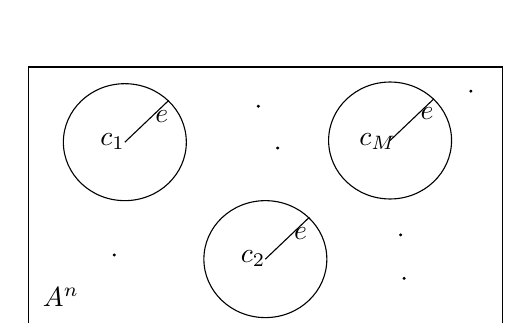
\begin{tikzpicture}[x=0.75pt,y=0.75pt,yscale=-1,xscale=1]
%uncomment if require: \path (0,438); %set diagram left start at 0, and has height of 438

%Shape: Rectangle [id:dp7021913647196929] 
\draw   (110,60) -- (338.5,60) -- (338.5,188) -- (110,188) -- cycle ;
%Shape: Ellipse [id:dp9765023649138487] 
\draw   (126.93,96.23) .. controls (126.93,80.67) and (140.19,68.05) .. (156.55,68.05) .. controls (172.91,68.05) and (186.17,80.67) .. (186.17,96.23) .. controls (186.17,111.79) and (172.91,124.4) .. (156.55,124.4) .. controls (140.19,124.4) and (126.93,111.79) .. (126.93,96.23) -- cycle ;
%Straight Lines [id:da44958964878480123] 
\draw    (156.55,96.23) -- (177.7,76.1) ;
%Shape: Ellipse [id:dp7217579776168563] 
\draw   (194.63,152.58) .. controls (194.63,137.02) and (207.89,124.4) .. (224.25,124.4) .. controls (240.61,124.4) and (253.87,137.02) .. (253.87,152.58) .. controls (253.87,168.14) and (240.61,180.75) .. (224.25,180.75) .. controls (207.89,180.75) and (194.63,168.14) .. (194.63,152.58) -- cycle ;
%Straight Lines [id:da6468705638620234] 
\draw    (224.25,152.58) -- (245.41,132.45) ;
%Shape: Ellipse [id:dp565989103161298] 
\draw   (254.72,95.42) .. controls (254.72,79.86) and (267.98,67.25) .. (284.34,67.25) .. controls (300.7,67.25) and (313.96,79.86) .. (313.96,95.42) .. controls (313.96,110.98) and (300.7,123.6) .. (284.34,123.6) .. controls (267.98,123.6) and (254.72,110.98) .. (254.72,95.42) -- cycle ;
%Straight Lines [id:da9666573745536973] 
\draw    (284.34,95.42) -- (305.49,75.3) ;
%Flowchart: Summing Junction [id:dp4148575963847989] 
\draw   (220.44,78.92) .. controls (220.44,78.7) and (220.63,78.52) .. (220.86,78.52) .. controls (221.1,78.52) and (221.29,78.7) .. (221.29,78.92) .. controls (221.29,79.14) and (221.1,79.32) .. (220.86,79.32) .. controls (220.63,79.32) and (220.44,79.14) .. (220.44,78.92) -- cycle ; \draw   (220.57,78.63) -- (221.16,79.2) ; \draw   (221.16,78.63) -- (220.57,79.2) ;
%Flowchart: Summing Junction [id:dp9659296963089476] 
\draw   (290.68,161.84) .. controls (290.68,161.61) and (290.87,161.43) .. (291.11,161.43) .. controls (291.34,161.43) and (291.53,161.61) .. (291.53,161.84) .. controls (291.53,162.06) and (291.34,162.24) .. (291.11,162.24) .. controls (290.87,162.24) and (290.68,162.06) .. (290.68,161.84) -- cycle ; \draw   (290.81,161.55) -- (291.41,162.12) ; \draw   (291.41,161.55) -- (290.81,162.12) ;
%Flowchart: Summing Junction [id:dp9540970746521595] 
\draw   (288.99,140.91) .. controls (288.99,140.68) and (289.18,140.5) .. (289.41,140.5) .. controls (289.65,140.5) and (289.84,140.68) .. (289.84,140.91) .. controls (289.84,141.13) and (289.65,141.31) .. (289.41,141.31) .. controls (289.18,141.31) and (288.99,141.13) .. (288.99,140.91) -- cycle ; \draw   (289.12,140.62) -- (289.71,141.19) ; \draw   (289.71,140.62) -- (289.12,141.19) ;
%Flowchart: Summing Junction [id:dp6406987067855436] 
\draw   (151.05,150.57) .. controls (151.05,150.34) and (151.23,150.16) .. (151.47,150.16) .. controls (151.7,150.16) and (151.89,150.34) .. (151.89,150.57) .. controls (151.89,150.79) and (151.7,150.97) .. (151.47,150.97) .. controls (151.23,150.97) and (151.05,150.79) .. (151.05,150.57) -- cycle ; \draw   (151.17,150.28) -- (151.77,150.85) ; \draw   (151.77,150.28) -- (151.17,150.85) ;
%Flowchart: Summing Junction [id:dp7345563398695256] 
\draw   (229.75,99.04) .. controls (229.75,98.82) and (229.94,98.64) .. (230.17,98.64) .. controls (230.41,98.64) and (230.6,98.82) .. (230.6,99.04) .. controls (230.6,99.27) and (230.41,99.45) .. (230.17,99.45) .. controls (229.94,99.45) and (229.75,99.27) .. (229.75,99.04) -- cycle ; \draw   (229.87,98.76) -- (230.47,99.33) ; \draw   (230.47,98.76) -- (229.87,99.33) ;
%Flowchart: Summing Junction [id:dp5030665895416562] 
\draw   (322.84,71.67) .. controls (322.84,71.45) and (323.03,71.27) .. (323.27,71.27) .. controls (323.5,71.27) and (323.69,71.45) .. (323.69,71.67) .. controls (323.69,71.9) and (323.5,72.08) .. (323.27,72.08) .. controls (323.03,72.08) and (322.84,71.9) .. (322.84,71.67) -- cycle ; \draw   (322.97,71.39) -- (323.57,71.96) ; \draw   (323.57,71.39) -- (322.97,71.96) ;

% Text Node
\draw (115.85,165.01) node [anchor=north west][inner sep=0.75pt]    {$A^{n}$};
% Text Node
\draw (143.47,90.85) node [anchor=north west][inner sep=0.75pt]    {$c_{1}$};
% Text Node
\draw (170.01,79.77) node [anchor=north west][inner sep=0.75pt]    {$e$};
% Text Node
\draw (211.17,147.2) node [anchor=north west][inner sep=0.75pt]    {$c_{2}$};
% Text Node
\draw (236.87,136.12) node [anchor=north west][inner sep=0.75pt]    {$e$};
% Text Node
\draw (268.26,90.85) node [anchor=north west][inner sep=0.75pt]    {$c_{M}$};
% Text Node
\draw (297.8,78.16) node [anchor=north west][inner sep=0.75pt]    {$e$};

\end{tikzpicture}
\end{center}

Let $n = 128$, $q = 2$, and $M = 2^{64}$. Does there exist a binary $[n, M]$-code with $d \geq 22$? 
If so, can encoding and decoding be done efficiently? 

We will construct such a code at the end of the course. The main tools used will be linear algebra 
(over finite fields) and abstract algebra (rings and fields).

\newpage 
\section{Finite fields}

\subsection{Introduction to finite fields}

\begin{defn}
A {\bf (commutative) ring} $(R, +, \cdot)$ consists of a set $R$, together with binary operations 
$+, \cdot : R \times R \to R$ such that 
\begin{enumerate}[(1)]
    \item $a + (b+c) = (a+b)+c$ for all $a, b, c, \in R$; 
    \item $a+b=b+a$ for all $a, b \in R$;
    \item there exists an element $0 \in R$ such that $a+0=a$ for all $a \in R$;
    \item for all $a \in R$, there exists an element $-a \in R$ such that $a+(-a) = 0$;
    \item $a \cdot (b \cdot c) = (a \cdot b) \cdot c$ for all $a, b, c \in R$;
    \item $a \cdot b = b \cdot a$ for all $a, b \in R$;
    \item there exists an element $1 \in R$ with $1 \neq 0$ such that $a \cdot 1 = a$ for all 
    $a \in R$; and 
    \item $a \cdot (b+c) = a \cdot b + a \cdot c$ for all $a, b, c \in R$.
\end{enumerate}
\end{defn}
We usually identify the ring $(R, +, \cdot)$ with just the set $R$. 

\begin{exmp}
The sets $\Z$, $\Q$, $\R$, and $\C$ equipped with their usual operations are all commutative rings. 
\end{exmp}

\begin{defn}
A field $(F, +, \cdot)$ is a commutative ring with the additional property that 
for all $a \in F \setminus \{0\}$, there exists an element $a^{-1} \in F$ such that 
$a \cdot a^{-1} = 1$.
\end{defn}

\begin{defn}
A field $(F, +, \cdot)$ is a {\bf finite field} if $F$ is finite; otherwise, it is an 
{\bf infinite field}. If $F$ is a finite field, its {\bf order} is given by $|F|$.
\end{defn}

\begin{exmp}
Note that $\Q$, $\R$, and $\C$ are all fields; in particular, they are infinite fields. 
However, $\Z$ is not a field, as $2$ does not have a multiplicative inverse in $\Z$.
\end{exmp}

We wish to answer the following questions:
\begin{enumerate}[(1)]
    \item For what integers $n \geq 2$ does there exist a finite field of order $n$?
    \item How does one construct such a field; that is, what are the elements of the field, 
    and how are the field operations performed?
\end{enumerate}

Let $n \geq 2$ be an integer. Recall that $\Z_n$ consists of the set of equivalence classes of integers 
modulo $n$, so $\Z_n = \{[0], [1], [2], \dots, [n-1]\}$ with addition and multiplication 
given by $[a] + [b] = [a+b]$ and $[a] \cdot [b] = [a \cdot b]$. More simply, we write 
$\Z_n = \{0, 1, 2, \dots, n-1\}$ (dropping the brackets) and perform addition and multiplication 
modulo $n$.

\begin{exmp}
For example, in $\Z_9 = \{0, 1, 2, \dots, 8\}$, we have $3+7=1$ and $3 \cdot 7 = 3$, since 
$3 + 7 \equiv 1 \; (\text{mod } 9)$ and $3 \cdot 7 \equiv 3 \; (\text{mod } 9)$.
\end{exmp}

\begin{remark}
It can be verified that $\Z_n$ is a commutative ring (axioms (1) to (8) all hold).
\end{remark}

\begin{thm}
Let $n \geq 2$. Then $\Z_n$ is a field if and only if $n$ is prime.
\end{thm}
\begin{pf}
For the forward direction, suppose that $n$ is prime. Suppose that $0 \neq a \in \Z_n$ so that 
$1 \leq a \leq n-1$. Since $n$ is prime, we have $\gcd(a, n) = 1$, and hence there 
exist $s, t \in \Z$ such that $as + nt = 1$. Reducing both sides modulo $n$ gives 
$as \equiv 1 \; (\text{mod } n)$. In particular, we have $a^{-1} = s$, and hence $\Z_n$ is a field. 

For the converse, suppose that $n$ is composite. That is, $n = ab$ for some $2 \leq a, b \leq n-1$. 
Suppose for a contradiction that $a^{-1}$ exists, so that $ac \equiv 1 \; (\text{mod } n)$ for 
some $c \in \Z_n$. Then $abc \equiv a \; (\text{mod } n)$, and so $nc \equiv a \; (\text{mod } n)$. 
Thus, $b \equiv 0 \; (\text{mod } n)$, which implies that $n \mid b$. But this is absurd, 
since we assumed that $2 \leq b \leq n-1$. Therefore, $\Z_n$ is not a field.
\end{pf}

Observe that Theorem 2.1.8 establishes the existence of finite fields of order $n$ for every 
prime $n$. What about finite fields of order $n$ where $n$ is composite?

\begin{defn}
Let $F$ be a field. The {\bf characteristic} of $F$, denoted $\ch(F)$, is the smallest integer 
$m$ such that 
\[ \underbrace{1 + \cdots + 1}_{\text{$m$ times}} = 0. \]
If no such $m$ exists, we define $\ch(F) = 0$. 
\end{defn}

\begin{exmp}
For prime $p$, the field $\Z_p$ has characteristic $p$. On the other hand, the fields 
$\Q$, $\R$, and $\C$ all have characteristic $0$.
\end{exmp}

\begin{thm}
Let $F$ be a field. If $\ch(F) = 0$, then $F$ is an infinite field. 
\end{thm}
\begin{pf}
Suppose for a contradiction that for positive integers $a < b$, we have
\[ \underbrace{1 + \cdots + 1}_{\text{$a$ times}} = \underbrace{1 + \cdots + 1}_{\text{$b$ times}}. \]
Then, we see that 
\[ \underbrace{1 + \cdots + 1}_{\text{$b$ times}} - \underbrace{1 + \cdots + 1}_{\text{$a$ times}} 
= \underbrace{1 + \cdots + 1}_{\text{$b-a$ times}} = 0, \]
which contradicts our assumption that $\ch(F) = 0$. Thus, the elements 
$1, 1+1, 1+1+1, \dots$ are all distinct, so $F$ must be infinite.
\end{pf}

\begin{thm}
Let $F$ be a field with $\ch(F) = m > 0$. Then $m$ is prime. 
\end{thm}
\begin{pf}
Suppose that $m$ is composite, say $m = ab$ where $2 \leq a, b \leq m-1$. Let 
$s = 1 + \cdots + 1$ ($a$ times) and $t = 1 + \cdots + 1$ ($b$ times), and note that 
$s, t \neq 0$. It follows that 
\[ s \cdot t = (\underbrace{1 + \cdots + 1}_{\text{$a$ times}}) \cdot 
(\underbrace{1 + \cdots + 1}_{\text{$b$ times}}) = 
\underbrace{1 + \cdots + 1}_{\text{$ab=m$ times}} = 0. \]
Thus, $s \cdot t \cdot t^{-1} = s \cdot 1 = s = 0$, a contradiction. Hence, $m$ must be prime.
\end{pf}

Let $F$ be a finite field of characteristic $p$. Consider the subset 
\[ E = \{0, 1, 1+1, 1+1+1, \dots, \underbrace{1 + \cdots + 1}_{\text{$p-1$ times}}\} \subseteq F. \]
The elements of $E$ are distinct, and it can be verified that $E$ is a field under the same 
operations as $F$. In particular, $E$ is a {\bf subfield} of $F$. Identifying the elements 
of $E$ with the elements of $\Z_p$ in the natural way, we see that $E$ is essentially the 
same field as $\Z_p$. That is, $\Z_p$ is a subfield of $F$.

Note that if $F$ is a finite field of characteristic $p$, then we can view $F$ 
as a vector space over $\Z_p$ (where the vectors are elements of $F$, and the 
scalars are elements of $\Z_p$).

\begin{thm}
Let $F$ be a finite field of characteristic $p$. Then the order of 
$F$ is $p^n$ for some integer $n \geq 1$.
\end{thm}
\begin{pf}
Let $n \geq 1$ be the dimension of $F$ viewed as a vector space over $\Z_p$. 
Let $\{\alpha_1, \dots, \alpha_n\}$ be a basis for $F$ over $\Z_p$. 
Then every element $\beta \in F$ can be written uniquely in the form 
\[ \beta = c_1\alpha_1 + \cdots + c_n\alpha_n, \]
where each $c_i \in \Z_p$. In particular, we have 
$F = \{\sum_{i=1}^n c_i\alpha_i : c_i \in \Z_p\}$, so $|F| = p^n$.
\end{pf}

As a consequence of Theorem 2.1.13, there do not exist finite fields of order $q$ when 
$q$ is not of the form $p^n$ where $p$ is prime and $n$ is a positive integer. 
However, given a fixed prime $p$ and positive integer $n$, do there exist finite fields 
$F$ such that $|F| = p^n$?

\subsection{Existence of finite fields}

\begin{defn}
Let $F$ be a field. We denote by $F[x]$ the set of all polynomials in $x$ with coefficients from $F$. 
Addition and multiplications of polynomials in $F[x]$ is done in the usual way, with 
coefficient arithmetic done in $F$. 
\end{defn}

\begin{exmp}
In $\Z_5[x]$, we have 
\[ (3x^4 + 2x^3 + x + 4) + (x^5 + 2x^4 + x^2 + 2x + 3) = x^5 + 2x^3 + x^2 + 3x + 2. \]
\end{exmp}

\begin{remark}
It can be shown that $F[x]$ is an infinite commutative ring.
\end{remark}

\begin{prop}[Division algorithm in $F{[x]}$]
Let $F$ be a field. Let $f, g \in F[x]$ with $g \neq 0$. Then there exist 
unique polynomials $s, r \in F[x]$ with $\deg(r) < \deg(g)$ such that 
$f = sg+r$. (By convention, we define $\deg(0) = -\infty$).
\end{prop}

\begin{exmp}
Let $f(x) = 3x^4 + 2x^3 + 2x^2 + x + 1,\, g(x) = 2x^2 + 3x+ 4 \in \Z_5[x]$. 
Then using the division algorithm in $\Z_5[x]$, we can find that 
\[ f(x) = (4x^2 + 3) g(x) + (2x+4), \]
so $s(x) = 4x^2 + 3$ and $r(x) = 2x+4$ are the unique polynomials $s, r \in 
\Z_5[x]$ with $\deg(r) < \deg(g)$ such that $f=sg+r$. 
\end{exmp}

\begin{defn}
Let $F$ be a field and let $f \in F[x]$ with $\deg(f) \geq 1$. Let 
$g, h \in F[x]$. Then {\bf $g$ is congruent to $h$ modulo $f$}, written 
$g \equiv h \; (\text{mod } f)$, if $g-h = \ell f$ for some $\ell \in F[x]$; 
equivalently, $f \mid g-h$. 
\end{defn}

The relation $\equiv (\text{mod } f)$ is an equivalence relation on $F[x]$, and 
partitions $F[x]$ into equivalence classes 
\[ [g] = \{h \in F[x] : h \equiv g \;(\text{mod } f)\}. \]
We can define addition and multiplication in the natural way; that is, 
$[g] + [h] = [g+h]$ and $[g] \cdot [h] = [g \cdot h]$. The set of equivalence classes is denoted by 
$F[x]/(f)$, and it can be verified that $F[x]/(f)$ is a commutative ring under the above operations.

Suppose now that $\deg(f) = n \geq 1$, and let $g \in F[x]$. Then we can write $g = sf+r$ where 
$s, r \in F[x]$ and $\deg(r) < n$. Notice that $g \equiv r \; (\text{mod } f)$, so 
$[g] = [r]$. Moreover, if $r_1, r_2 \in F[x]$ with $r_1 \neq r_2$ and $\deg(r_1), \deg(r_2) < n$, 
then $f \nmid r_1 - r_2$, so $r_1 \not\equiv r_2 \; (\text{mod } f)$. Thus, 
$[r_1] \neq [r_2]$. Therefore, the polynomials in $F[x]$ of degree less than $n$ are a 
{\bf complete set of representatives} of the equivalence classes of $F[x]/(f)$.

Now, let $F = \Z_p$. Then $\Z_p[x]/(f) = \{[r] : r \in \Z_p[x],\, \deg(r) < n\}$. 
We can see that $|\Z_p[x]/(f)| = p^n$, so $\Z_p[x]/(f)$ is a finite commutative ring of 
order $p^n$. But when is $\Z_p[x]/(f)$ a field?

\begin{defn}
Let $F$ be a field and let $f \in F[x]$ with $\deg(f) \geq 1$. Then 
$f$ is {\bf irreducible over $F$} if $f$ cannot be written as $f = gh$ where 
$g, h \in F[x]$ with $\deg(g), \deg(h) \geq 1$. Otherwise, we say that $f$ 
is {\bf reducible over $F$}.
\end{defn}

\begin{exmp}
Let $f(x) = x^2 + 1$.
\begin{itemize}
    \item $f(x)$ is irreducible over $\R$ since it has no roots in $\R$. 
    \item $f(x)$ is reducible over $\C$ since we have $f(x) = (x+i)(x-i)$. 
    \item $f(x)$ is reducible over $\Z_2$ since we can write $f(x) = (x+1)(x+1)$.
    \item $f(x)$ is irreducible over $\Z_3$ since it has no roots in $\Z_3$.
\end{itemize}
\end{exmp}

\begin{thm}
Let $F$ be a field and let $f \in F[x]$ with $\deg(f) \geq 1$. Then 
$F[x]/(f)$ is a field if and only if $f$ is irreducible over $F$. 
\end{thm}
\begin{pf}
Analogous to the proof of Theorem 2.1.8 (which states that $\Z_n$ is a field if and only if $n$ is prime).
\end{pf}

We conclude that if $f \in \Z_p[x]$ is irreducible with $\deg(f) = n \geq 1$, 
then $\Z_p[x]/(f)$ is a finite field of order $p^n$ and 
characteristic $p$. The elements of $\Z_p[x]/(f)$ are the polynomials in 
$\Z_p[x]$ of degree less than $n$.

\begin{exmp}
Let $p = 2$ and $n = 2$. Let $f(x) = x^2 + x + 1 \in \Z_2[x]$.
Then $f(0) = f(1) = 1$, so $f$ has no roots in $\Z_2$. Hence, $f$ is irreducible over $\Z_2$, 
and thus $F = \Z_2[x]/(x^2 + x + 1)$ is a finite field of order $2^2 = 4$. The 
elements of $F$ are $\{0, 1, x, x+1\}$.
\end{exmp}

\begin{exmp}
Let $p = 2$ and $n = 3$. To obtain a finite field of order $2^3 = 8$, we need to find an 
irreducible polynomial of degree $3$ over $\Z_2$. Indeed, consider 
$f(x) = x^3 + x + 1$. Since $f(0) = f(1) = 1$, we see that $f$ has no roots in $\Z_2$, 
and hence is irreducible over $\Z_2$. Thus, $F = \Z_2[x]/(x^3 + x + 1)$ is a finite 
field of order $8$. The elements of $F$ are 
$\{0, 1, x, x+1, x^2, x^2+1, x^2+x, x^2+x+1\}.$
\end{exmp}

\begin{remark}
Note that in the above example, we also could have chosen $g(x) = x^3 + x^2 + 1$ 
as our irreducible polynomial of degree $3$ over $\Z_2$. Then 
$F' = \Z_2[x]/(x^3 + x^2 + 1)$ is also a finite field of order $8$ with elements 
$\{0, 1, x, x+1, x^2, x^2+1, x^2+x, x^2+x+1\}.$

We note that $F$ and $F'$ are {\it not} the same field. Notice that in 
$F$, we have $x \cdot x^2 = x+1$, whereas in $F'$, we have 
$x \cdot x^2 = x^2 + 1$. Nonetheless, $F$ and $F'$ are {\bf isomorphic}; 
that is, there is a bijection $\phi : F \to F'$ such that 
$\phi(a+b) = \phi(a) + \phi(b)$ and $\phi(a \cdot b) = \phi(a) \cdot \phi(b)$ for all 
$a, b \in F$.
\end{remark}

Finally, we list some useful facts. 
\begin{itemize}
    \item Let $p$ be prime and $n$ be a positive integer. Then there exists an irreducible 
    polynomial of degree $n$ over $\Z_p$.
    \item There exists a finite field of order $q$ if and only if $q = p^n$ 
    for some prime $p$ and positive integer $n$.
    \item Any two fields of the same order are isomorphic.
\end{itemize}
\begin{defn} 
We will denote {\it the} finite field of order $q$ (up to isomorphism) 
by $\GF(q)$, and call it the {\bf Galois field of order $q$}.
\end{defn}

We summarize our results in the following diagram. 
\begin{table}[h]
\centering
\begin{tabular}{ccccc}\vspace{3ex}
{\bf Infinite ring} &                                                                                                                                                                                                  & {\bf Finite ring} &                  & {\bf Finite field}                                                               \\\vspace{3ex}
$\Z$                                                                  & 
$\xrightarrow[a \equiv b\;(\text{mod } n)]{\text{Let } n \geq 2}$ & $\Z_n$                                                              & $\xrightarrow{n \text{ prime}}$ & \begin{tabular}[c]{@{}c@{}}$\Z_n$, order $n$\end{tabular}          \\
$\Z_p[x]$                                                             & 
$\xrightarrow[g \equiv h\;(\text{mod } f)]{\text{Let } f \in \Z_p[x],\, \deg(f) = n \geq 1}$ & $\Z_p[x]/(f)$                                                       & $\xrightarrow{f \text{ irreducible}}$  & $\Z_p[x]/(f)$, order $p^n$
\end{tabular}
\end{table}

\subsection{Properties of finite fields}

\begin{thm}[Freshman's dream]
Let $F$ be a field of characteristic $p$, and let $\alpha, \beta \in F$. Then for all $m \geq 1$, 
we have 
\[ (\alpha+\beta)^{p^m} = \alpha^{p^m} + \beta^{p^m}. \]
\end{thm}
\begin{pf}
We proceed by induction on $m$. For $m = 1$, it follows from the Binomial Theorem that 
\[ (\alpha + \beta)^p = \binom{p}0 \alpha^p + \sum_{i=1}^{p-1} \alpha^i \beta^{p-i} + \binom{p}p \beta^p. \]
Observe that for all $1 \leq i \leq p-1$, we have 
\[ \binom{p}{i} = \frac{p(p-1)(p-2) \cdots (p-i+1)}{i(i-1) \cdots (1)} \equiv 0 \pmod p, \]
since $\binom{p}{i}$ is an integer and $p$ divides the numerator but not the numerator. 
Thus, for each $1 \leq i \leq p-1$, we obtain 
\[ \binom{p}{i} \alpha^i \beta^{p-i} = \underbrace{\alpha^i \beta^{p-i} + \cdots + 
\alpha^i \beta^{p-i}}_{\text{$\binom{p}i$ times}} = 
\underbrace{(1 + \cdots + 1)}_{\text{$\binom{p}i$ times}} \alpha^i \beta^{p-i} = 0. \]
Hence, $(\alpha + \beta)^p = \alpha^p + \beta^p$. We leave the inductive case as an exercise.
\end{pf}

\begin{defn}
The {\bf multiplicative group of $\GF(q)$} is the set $\GF(q)^* = \GF(q) \setminus \{0\}$.
\end{defn}

The following theorem is a generalization of Fermat's Little Theorem for $\GF(q)$. 

\begin{thm}
If $\alpha \in \GF(q)^*$, then $\alpha^{q-1} = 1$. 
\end{thm}
\begin{pf}
Let us denote the distinct elements of $\GF(q)^*$ by $\alpha_1, \dots, \alpha_{q-1}$. 
Consider the non-zero elements $\alpha\alpha_1, \dots, \alpha\alpha_{q-1}$. 
Note that these elements are also distinct, because if $\alpha\alpha_i = \alpha\alpha_j$ for 
some $i\neq j$, then this would imply that $\alpha_i = \alpha^{-1}(\alpha\alpha_i) 
= \alpha^{-1}(\alpha\alpha_j) = \alpha_j$, a contradiction. Hence, we have 
$\{\alpha\alpha_1, \dots, \alpha\alpha_{q-1}\} = \{\alpha_1, \dots, \alpha_{q-1}\}$, 
and so 
\[ (\alpha\alpha_1)(\alpha\alpha_2) \cdots (\alpha\alpha_{q-1}) = \alpha_1\alpha_2 \cdots 
\alpha_{q-1}. \]
Cancelling out terms on both sides, it follows that $\alpha^{q-1} = 1$.
\end{pf}

\begin{cor}
If $\alpha \in \GF(q)$, then $\alpha^q = \alpha$.
\end{cor}
\begin{pf}
If $\alpha \in \GF(q)^*$, then by Theorem 2.3.3, we have $\alpha^q = \alpha\alpha^{q-1} 
= \alpha \cdot 1 = \alpha$. Otherwise, we have $\alpha = 0$, and it is clear that 
$0^q = 0$.
\end{pf}

\begin{defn}
Let $\alpha \in \GF(q)^*$. The {\bf order} of $\alpha$, denoted $\ord(\alpha)$, is the 
smallest positive integer $t$ such that $\alpha^t = 1$. 
\end{defn}

\begin{remark}
There is only one element in $\GF(q)$ of order $1$, namely the element $1$.
\end{remark}

\begin{thm}
Let $\alpha \in \GF(q)^*$ with $\ord(\alpha) = t$. Then $\alpha^s = 1$ if and only if $t \mid s$.
\end{thm}
\begin{pf}
Suppose $s \in \Z$. Then long division of $s$ by $t$ yields $s = \ell t + r$ for some $0 \leq r < t$. 
We then see that 
\[ \alpha^s = \alpha^{\ell t + r} = (\alpha^t)^\ell \cdot \alpha^r = \alpha^r. \]
Note that $\alpha^s = 1$ if and only $r = 0$, and $r = 0$ if and only if $t \mid s$, so the result 
follows.
\end{pf}

\begin{cor}
If $\alpha \in \GF(q)^*$, then $\ord(\alpha) \mid q-1$. 
\end{cor}
\begin{pf}
Apply Theorem 2.3.3 and Theorem 2.3.7.
\end{pf}

\begin{exmp}
Consider the field $\GF(2^3) = \Z_2[x]/(x^3 + x + 1)$. The order of $x^2 + 1$ is $7$, 
since the order cannot be $1$ (by Remark 2.32) and must divide $2^3 - 1 = 7$. 
\end{exmp}

\begin{exmp}
Note that $x^4 + x + 1$ is irreducible over $\Z_2$ (check this). Consider the field 
$\GF(2^4) = \Z_2[x]/(x^4 + x + 1)$. Observe that $x^1 = x$, $x^3 = x^3$, and 
$x^5 = x^2 + x$, none of which are equal to $1$, so $\ord(x)$ cannot be equal to $1$, $3$, or $5$. 
Since $\ord(x) \mid 15$, it must be that $\ord(x) = 15$. 
\end{exmp}

\begin{remark}
If $\alpha \in \GF(q)^*$ with $\ord(\alpha) = t$, then the elements 
$\alpha^0, \alpha^1, \alpha^2, \dots, \alpha^{t-1}$ are distinct. In particular, if 
$\ord(\alpha) = q-1$, then $\GF(q)^* = \{\alpha^0, \alpha^1, \alpha^2, \dots, \alpha^{q-2}\}$.
\end{remark}

\begin{defn}
A {\bf generator} of $\GF(q)^*$ is an element of order $q-1$.
\end{defn}

\begin{exmp}
As seen in Example 2.3.10, $x$ is a generator of $\GF(2^4) = \Z_2[x]/(x^4 + x + 1)$ since 
$\ord(x) = 15$.
\end{exmp}

Note that every finite field $\GF(q)$ has a generator, but we will not prove this fact here.

\newpage 
\section{Linear codes} 

\subsection{Introduction to linear codes}

We first introduce some notation. We will denote $F = \GF(q)$, and define 
$V_n(F) := F^n$. Note that $V_n(F)$ is an $n$-dimensional vector space over $F$ with 
$|V_n(F)| = q^n$. 

\begin{defn}
A {\bf linear $(n, k)$-code over $F$} is a $k$-dimensional subspace of $V_n(F)$.
\end{defn}

Let $C$ be an $(n, k)$-code over $F$, and let $\{v_1, \dots, v_k\}$ be an ordered basis for $C$. 
We list some properties of $C$. 

{\bf Number of codewords.} The elements of $C$ are precisely 
\[ c_1 v_1 + \cdots + c_k v_k, \]
where each $c_i \in F$. Thus, $|C| = M = q^k$. 

{\bf Information rate.} The rate of $C$ is $R = (\log_q M)/n = (\log_q q^k)/n = k/n$. 

{\bf Weight.} Consider the following definition and theorem. 

\begin{defn}
The {\bf Hamming weight} $w(v)$ of a vector $v \in F_n(F)$ is the number of non-zero coordinates in $v$.
The {\bf Hamming weight} of a linear code $C$ is given by 
\[ w(C) := \{w(c) : c \in C,\, c \neq 0\}. \]
\end{defn}

\begin{thm}
If $C$ is a linear code, then $w(C) = d(C)$.
\end{thm}
\begin{pf}
We have 
\begin{align*}
d(C) &= \min\{d(x, y) : x, y \in C,\, x \neq y\} \\
&= \min\{w(x - y) : x, y \in C,\, x \neq y\} \text{ (since $d(x, y) = w(x-y)$)} \\
&= \min\{w(c) : c \in C,\, c \neq 0\} \text{ (since $C$ is linear, $x - y \in C$)} \\
&= w(C). \qedhere 
\end{align*}
\end{pf}

{\bf Encoding.} Since there are $q^k$ codewords, there are also $q^k$ source messages. We shall
assume that the source messages are the elements of $F^k$. Then a convienient and 
natural bijection (known as an {\bf encoding rule}) between $F^k$ and $C$ is given by 
\[ m = (m_1, \dots, m_k) \mapsto c = m_1v_1 + \cdots + m_kv_k. \]

{\bf Generator matrix.} This gives us a convenient way of representing $C$. 

\begin{defn}
A {\bf generator matrix} $G$ for an $(n, k)$-code $C$ is a $k \times n$ matrix whose rows 
from a basis for $C$; that is, with the ordered basis $\{v_1, \dots, v_k\}$ for $C$, 
we have 
\[ G = \begin{bmatrix} v_1 \\ \vdots \\ v_k \end{bmatrix}_{k\times n}. \]
\end{defn}

Note that the encoding rule above is more compactly stated as $c = mG$. 

\begin{exmp}
Consider the binary $(5, 3)$-code 
\[ C = \langle c_1 = 10011, c_2 = 01001, c_3 = 00110 \rangle, \]
where $c_1, c_2, c_3$ are linearly independent over $\GF(2)$. A generator matrix for $C$ is 
\[ G = \begin{bmatrix} 1 & 0 & 0 & 1 & 1 \\ 0 & 1 & 0 & 0 & 1 \\ 0 & 0 & 1 & 1 & 0 \end{bmatrix}. \]
The encoding rule (with respect to the ordered basis $\{c_1, c_2, c_3\}$) is $c = mG$. More explicitly, 
we have 

\begin{table}[H]
\centering
\begin{tabular}{ccc}
$m$   &               & $c$     \\
      &               &         \\
$000$ & $\rightarrow$ & $00000$ \\
$001$ & $\rightarrow$ & $00110$ \\
$010$ & $\rightarrow$ & $01001$ \\
$011$ & $\rightarrow$ & $01111$ \\
$100$ & $\rightarrow$ & $10011$ \\
$101$ & $\rightarrow$ & $10101$ \\
$110$ & $\rightarrow$ & $11010$ \\
$111$ & $\rightarrow$ & $11100$
\end{tabular}
\end{table}

Moreover, we clearly have $M = |C| = 2^3 = 8$, $R = 3/5$, and $d(C) = w(C) = 2$. 
\end{exmp}

\begin{defn}
Let $C$ be an $(n, k)$-code over $F$. A generator matrix $G$ for $C$ of the form 
\[ G = \begin{bmatrix} I_k \mid A \end{bmatrix}_{k\times n} \]
is said to be in {\bf standard form}. If $C$ has a generator matrix in standard form, 
then $C$ is a {\bf systematic code}.
\end{defn}

\begin{exmp}
The code $C = \langle 100011, 001001, 000110 \rangle$ is a non-systematic $(6, 3)$-code. 
On the other hand, $C' = \langle 100011, 001001, 010010 \rangle$ is a systematic code, 
since the generator matrix 
\[ G = \begin{bmatrix} 1 & 0 & 0 & 0 & 1 & 1 \\ 0 & 1 & 0 & 0 & 1 & 0 \\ 0 & 0 & 1 & 0 & 0 & 1 
\end{bmatrix} \]
for $C'$ is in standard form.
\end{exmp}

\begin{defn}
Two codes $C$ and $C'$ over $F$ are {\bf equivalent} if $C'$ can be obtained from $C$
by choosing a permutation of the coordinate positions $\{1, 2, \dots, n\}$, and 
then consistently rearranging every codeword of $C$ according to this permutation.
\end{defn}

\begin{exmp}
The codes $C$ and $C'$ from Example 3.1.7 are equivalent; in particular, the 
second and fourth coordinates were swapped.
\end{exmp}

The following facts are easy to prove.
\begin{enumerate}[(1)]
    \item If $C$ is linear and $C'$ is equivalent to $C$, then $C'$ is linear.
    \item Equivalent codes have the same length, dimension, and distance.
    \item Every linear code is equivalent to a systematic code.
\end{enumerate}

\subsection{Dual codes and parity-check matrices}

\begin{defn}
Let $x = (x_1, \dots, x_n),\, y = (y_1, \dots, y_n) \in V_n(F)$. The {\bf inner product} of 
$x$ and $y$ is defined to be 
\[ x \cdot y = \sum_{i=1}^n x_iy_i \in F. \]
\end{defn}

\begin{exmp}
Suppose that $x = (2, 0, 1, 1),\, y = (2, 0, 2, 1) \in V_4(\Z_3)$. Then $x \cdot y = 1$. 
\end{exmp}

Observe that for all $x, y, z \in V_n(F)$ and $\lambda \in F$, we have 
\begin{enumerate}[(i)]
    \item $x \cdot y = y \cdot x$;
    \item $x \cdot (y+z) = x \cdot y + x \cdot z$; and 
    \item $(\lambda x) \cdot y = \lambda(x \cdot y)$. 
\end{enumerate}

\begin{remark}
Note that $x \cdot x = 0$ does not necessarily imply that $x = 0$. Indeed, consider 
$x = 111100 \in V_6(\Z_2)$. Then $x \cdot x = 0$, but $x \neq 0$. More generally, if 
$x \in V_n(\Z_2)$, then $x \cdot x = 0$ if and only if $w(x)$ is even. 
\end{remark}

\begin{defn}
Two vectors $x, y \in V_n(F)$ are said to be {\bf orthogonal} if $x \cdot y = 0$. 
\end{defn}

We now take a look at the notion of the dual code of a linear code. 

\begin{defn}
Let $C$ be an $(n, k)$-code over $F$. The {\bf dual code} (or {\bf orthogonal code}) of $C$ 
is the code 
\[ C^\perp := \{x \in V_n(F) : x \cdot y \text{ for all } y \in C\}. \]
\end{defn}

\begin{thm}
If $C$ is an $(n, k)$-code over $F$, then $C^\perp$ is an $(n, n-k)$-code over $F$. 
\end{thm}
\begin{pf}
Let $G$ be a generator matrix of $C$, and denote the rows of $G$ by $v_1, \dots, v_k$. 

{\sc Claim.} If $x \in V_n(F)$, then $x \in C^\perp$ if and only if $v_1 \cdot x = 
v_2 \cdot x = \cdots = v_k \cdot x = 0$. 

{\sc Proof of Claim.} The forward direction is clear, since $v_1, \dots, v_k \in C$. For the 
converse, suppose $v \in C$. Then we can write $v = \lambda_1v_1 + \cdots + \lambda_kv_k$ 
where each $\lambda_i \in F$. We see that 
\[ v \cdot x = (\lambda_1v_1 + \cdots + \lambda_kv_k) \cdot x 
= \lambda(v_1 \cdot x) + \cdots + \lambda_k(v_k \cdot x) = 0, \]
and since $v \in C$ was arbitrary, we have $x \in C^\perp$. \hfill $\blacksquare$

By the claim, we see that $C^\perp = \{x \in V_n(F) : Gx^T = 0\}$ is the null space of $G$. 
Since $G$ has rank $k$, it follows that $C^\perp$ is a subspace of $V_n(F)$ of dimension $n-k$. 
\end{pf}

\begin{thm}
If $C$ is a linear code, then $(C^\perp)^\perp = C$. 
\end{thm}
\begin{pf}
Let $C$ be an $(n, k)$-code. By Theorem 3.2.6, $C^\perp$ is an $(n, n-k)$-code, 
and applying Theorem 3.2.6 once more, we have that $(C^\perp)^\perp$ is an $(n, k)$-code. 
Moreover, if $x \in C$, then for all $y \in C^\perp$, we have $x \cdot y = 0$, so 
$C \subseteq (C^\perp)^\perp$. Since $\dim(C) = \dim((C^\perp)^\perp) = k$, it follows that 
$C = (C^\perp)^\perp$. 
\end{pf}

\begin{defn}
If $C$ is a linear code, then a generator matrix $H$ for $C^\perp$ is called a 
{\bf parity-check matrix} for $C$. 
\end{defn}

\begin{remark}
Let $C$ be an $(n, k)$-code.
\begin{enumerate}[(1)]
    \item Since $C^\perp$ is an $(n, n-k)$-code, a parity-check matrix for $C$ is an 
    $(n-k)\times n$ matrix. 
    \item Since $C$ has many generator matrices, we see that $C$ also has many parity-check matrices. 
\end{enumerate}
\end{remark}

\begin{thm}
Let $C$ be an $(n, k)$-code with generator matrix $[I_k \mid A]$, where $A$ is a 
$k \times (n-k)$ matrix. Then $H = [-A^T \mid I_{n-k}]$ is a generator matrix for 
$C^\perp$. 
\end{thm}
\begin{pf}
Since $\rank(H) = n-k$, we see that $H$ is a generator matrix for an $(n, n-k)$-code $\overline{C}$. 
Also, observe that 
\[ GH^T = \begin{bmatrix} I_k \mid A \end{bmatrix} 
\left[
\begin{array}{c}
-A \\
\hline
I_{n-k}
\end{array}
\right] = 
-A + A = 0. \]
Thus, $\overline{C} \subseteq C^\perp$. Since $\dim(\overline{C}) = \dim(C^\perp)$, 
we have $\overline{C} = C^\perp$. Hence, $H$ is a generator matrix for $C^\perp$. 
\end{pf}

\begin{exmp}
Consider the $(5, 2)$-code $C$ over $\Z_3$ with generator matrix 
\[ G = \begin{bmatrix} 2 & 0 & 2 & 1 & 0 \\ 1 & 1 & 0 & 0 & 1 \end{bmatrix}. \]
Let us find a parity-check matrix for $C$. First, we need to find a generator matrix 
for $C$ in standard form. Indeed, performing some row operations, we obtain 
\[ G \xrightarrow[]{R_1 \leftarrow 2R_1} \begin{bmatrix} 1 & 0 & 1 & 2 & 0 \\ 1 & 1 & 0 & 0 & 1 
\end{bmatrix} \xrightarrow[]{R_2 \leftarrow R_2 - R_1} 
\begin{bmatrix} 1 & 0 & 1 & 2 & 0 \\ 0 & 1 & 2 & 1 & 1 \end{bmatrix}. \]
By Theorem 3.2.10, it follows that 
\[ H = \begin{bmatrix} 2 & 1 & 1 & 0 & 0 \\ 1 & 2 & 0 & 1 & 0 \\ 0 & 2 & 0 & 0 & 1 \end{bmatrix} \]
is a parity-check matrix for $C$. 
\end{exmp}

\subsection{Distance of a linear code}

Looking just at a parity-check matrix of a linear code $C$, we can say something about the 
distance of $C$. 

\begin{thm}
Let $H$ be a parity-check matrix for an $(n, k)$-code $C$ over $F$. Let $s \geq 2$. 
Then $d(C) \geq s$ if and only if every $s-1$ columns of $H$ are linearly independent over $F$.
\end{thm}
\begin{pf}
Let the columns of $H$ be $h_1, \dots, h_n$. 

$(\Leftarrow)$ Suppose that $d(C) \leq s-1$. Let $c = (c_1, \dots, c_n) \in C$ be a codeword 
with $1 \leq w(c) \leq s-1$. Without loss of generality, suppose that $c_j = 0$
for all $s \leq j \leq n$. Since $Hc^T = 0$, we have 
\[ c_1h_1 + c_2h_2 + \cdots + c_{s-1}h_{s-1} + c_sh_s + \cdots + c_nh_n = 0, \]
and hence $c_1h_1 + \cdots + c_{s-1}h_{s-1} = 0$. Since at least one of $c_1, \dots, c_{s-1}$ 
is non-zero, the $s-1$ columns $h_1, \dots, h_{s-1}$ are linearly dependent over $F$. 

$(\Rightarrow)$ Suppose there is a set of $s-1$ columns of $H$ which is linearly dependent over $F$. 
Without loss of generality, suppose these columns are $h_1, \dots, h_{s-1}$. Then, there 
exist scalars $\lambda_1, \dots, \lambda_{s-1} \in F$, not all zero, such that 
\[ \lambda_1h_1 + \lambda_2 h_2 + \cdots + \lambda_{s-1} h_{s-1} = 0. \]
Let $c = (\lambda_1, \dots, \lambda_{s-1}, 0, \dots, 0) \in V_n(F)$. Then $c \in C$ 
since $Hc^T = \lambda_1h_1 + \cdots + \lambda_{s-1}h_{s-1} = 0$. But $1 \leq w(c) \leq s-1$, 
so $1 \leq d(C) \leq s-1$. 
\end{pf}

As a direct consequence of Theorem 3.3.1, we have the following corollary. 

\begin{cor}
Let $H$ be a parity-check matrix for a linear code $C$ over $F$. Then $d(C)$ is the smallest 
number of columns of $H$ that are linearly dependent over $F$. 
\end{cor}

\begin{exmp}
Recall Example 3.2.11, where we had a code $C$ over $\Z_3$ with parity-check matrix 
\[ H = \begin{bmatrix} 2 & 1 & 1 & 0 & 0 \\ 1 & 2 & 0 & 1 & 0 \\ 0 & 2 & 0 & 0 & 1 \end{bmatrix}. \]
\begin{itemize}
    \item No single column of $H$ is linearly dependent over $\Z_3$ (as there is no zero column), 
    so $d(C) \geq 2$. 
    \item No two columns of $H$ are linearly dependent over $\Z_3$ (there are no scalar multiples of 
    each other), so $d(C) \geq 3$. 
    \item There exist three columns of $H$ which are linearly dependent over $\Z_3$. Indeed, we have 
    \[ \begin{bmatrix} 2\\1\\0\end{bmatrix} - 2\begin{bmatrix}1\\0\\0\end{bmatrix} 
    - \begin{bmatrix}0\\1\\0\end{bmatrix} = \begin{bmatrix}0\\0\\0\end{bmatrix}, \]
    so $d(C) \leq 3$. 
\end{itemize}
Thus, it follows that $d(C) = 3$. 
\end{exmp}

\begin{exmp}
Let $H$ be a parity-check matrix for a binary linear code $C$. 
\begin{enumerate}[(1)]
    \item We have $d(C) = 1$ if and only if $H$ has a zero column. 
    \item We have $d(C) = 2$ if and only if $H$ has no zero column, and two columns of $H$ are the same.
    \item We have $d(C) = 3$ if and only if the columns of $H$ are non-zero and distinct, 
    and some column is the sum of two other columns. 
\end{enumerate}
\end{exmp}

\begin{exmp}
By our observations in Example 3.3.4, we can construct a binary $(7, 4, 3)$-code over $C$; 
that is, a binary $(7, 4)$-code with distance $3$. First, we construct a parity-check matrix for $C$. 
Consider 
\[ H = \left[
\begin{array}{ccc|cccc}
1 & 0 & 0 \;&\; 1 & 0 & 1 & 1 \\ 0 & 1 & 0 \;&\; 1 & 1 & 0 & 1 \\ 0 & 0 & 1 \;&\; 0 & 
1 & 1 & 1 \end{array}
\right] \]
which has no zero column, and all columns are distinct. Moreover, we can see that the fourth 
column is the sum of the first two columns, so $d(C) = 3$. Then, a generator matrix for $C$ is 
given by 
\[ G = \left[
\begin{array}{ccc|cccc}
1 & 1 & 0 \;&\; 1 & 0 & 0 & 0 \\
0 & 1 & 1 \;&\; 0 & 1 & 0 & 0 \\ 
1 & 0 & 1 \;&\; 0 & 0 & 1 & 0 \\ 
1 & 1 & 1 \;&\; 0 & 0 & 0 & 1 \end{array}
\right]. \]
The code $C$ is simply the set of linear combinations of the rows of $G$. 
\end{exmp}

\subsection{Hamming codes}

We now focus on Hamming codes, which is an infinite family of single-error correcting codes discovered by Richard 
Hamming in 1950. 

\begin{defn}
A {\bf Hamming code of order $r$ over $F = \GF(q)$} is an $(n, k)$-code over $F$ with 
$n = (q^r - 1)/(q-1)$, $k = n-r$, and parity-check matrix $H_r$ being an $r \times n$ matrix 
whose columns are non-zero and no two of whose columns are scalar multiples of each other. 
\end{defn}

\begin{defn}
The binary $(7, 4, 3)$-code $C$ in Example 3.3.5 is a Hamming code of order $3$ over $\Z_2$. 
\end{defn}

\begin{exmp}
A parity-check matrix for a Hamming code of order $3$ over $\Z_3$ is given by 
\[ H_3 = \left[
\begin{array}{ccc|ccc|c|ccc|ccc}
1 & 0 & 0 \;&\; 1 & 1 & 0 \;&\; 1 \;&\; 2 & 1 & 0 \;&\; 1 & 1 & 2 \\
0 & 1 & 0 \;&\; 1 & 0 & 1 \;&\; 1 \;&\; 1 & 0 & 2 \;&\; 1 & 2 & 1 \\ 
0 & 0 & 1 \;&\; 0 & 1 & 1 \;&\; 1 \;&\; 0 & 2 & 1 \;&\; 2 & 1 & 1 \end{array}
\right]. \] 
Note that we have $n = 13$, $k = 10$, and $d = 3$. 
\end{exmp}

\begin{remark}~
\begin{enumerate}[(1)]
    \item If $v \in V_r(F)$ with $v \neq 0$, then exactly one scalar multiple of $v$ is a column 
    of $H_r$ (giving $n = (q^r - 1)/(q-1)$ columns in total).
    \item The matrix $H_r$ has rank $r$, since among its columns are scalar multiples of 
    the unit vectors. Hence, a Hamming code of order $r$ over $\GF(q)$ does indeed have dimension 
    $k = n-r$. 
    \item A Hamming code of order $r$ over $\GF(q)$ has distance $3$ (by design), so it is 
    a single-error correcting code by Theorem 1.3.6. 
\end{enumerate}
\end{remark}

For the remainder of this section, let $H$ be a parity-check matrix of an $(n, k, d)$-code $C$ 
over $F$ with $d \geq 3$. 

\begin{defn}
Suppose that $c \in C$ is sent, and $r \in V_n(F)$ is received. The {\bf error vector} 
is given by $e = r-c$ (or equivalently, $r = c+e$). 
\end{defn}

\begin{exmp}
Over $\Z_3$, if $c = 100100$ is sent and $r = 120101$ is received, then $e = 020000$. 
\end{exmp}

With the notion of an error vector, we can make the following observations.
\begin{enumerate}[(1)]
    \item We have $Hr^T = H(c+e)^T = Hc^T + He^T = He^T$. 
    \item If $e = 0$, then $He^T = 0$. (The converse is not true.)
    \item If $w(e) = 1$, say $e = (0, \dots, 0, \alpha, 0, \dots, 0)$ where $\alpha$ is at the 
    $i$-th position, then $He^T = \alpha h_i$ where $h_i$ is the $i$-th column of $H$ which is 
    non-zero by design. (The converse is not true.)
\end{enumerate}
This suggests the following decoding algorithm. 

\begin{algo}
We are given a parity-check matrix $H$ and a received word $r$. 
\begin{enumerate}[(1)]
    \item Compute $s = Hr^T$. 
    \item If $s = 0$, then accept $r$ as the transmitted word (in this case, we have $e = 0$). 
    \item If $s \neq 0$, then compare $s$ with the columns of $H$. If $s = \alpha h_i$ for some 
    $\alpha \in F$ and column $h_i$ of $H$, then set $e = (0, \dots, 0, \alpha, 0, \dots, 0)$
    with $\alpha$ at the $i$-th position, and decode $r$ to $c = r-e$. 
    \item Otherwise, report that more than one error has occurred. 
\end{enumerate}
\end{algo}
If $w(e) = 0$ or $w(e) = 1$, then this decoding algorithm is guaranteed to make the correct decision. 

\begin{exmp}
Consider the $(7, 4, 3)$-binary Hamming code with parity-check matrix 
\[ H = \begin{bmatrix} 
1 & 0 & 1 & 0 & 1 & 0 & 1 \\ 0 & 1 & 1 & 0 & 0 & 1 & 1 \\ 0 & 0 & 0 & 1 & 1 & 1 & 1 \end{bmatrix}. \]
Suppose that $r = 0111110$ is received. We see that 
\[ s = Hr^T = \begin{bmatrix} 0 \\ 1 \\ 1 \end{bmatrix}, \]
which is the sixth column of $H$. Hence, we set $e = 0000010$ and decode $r$ to $c = 
r-e = 0111100$. To check that this is correct, we can verify that $Hc^T = 0$. 
\end{exmp}

\subsection{Perfect codes}

\begin{defn}
Let $C$ be an $[n, M]$-code of distance $d$ over $A$, with $|A| = q$ and $e = \lfloor (d-1)/2 \rfloor$. 
Then $C$ is {\bf perfect} if each $x \in A^n$ is contained in the sphere of radius $e$ centered 
at some $c \in C$. Equivalently, $C$ is perfect if it attains the sphere packing bound; that is, 
we have 
\[ M \cdot \sum_{i=0}^e \binom{n}{i} (q-1)^i = q^n. \]
\end{defn}

For fixed $q$, $n$, and $d$, a perfect code has maximum possible $M$. In other words, a perfect code 
has maximum possible information rate $R = (\log_q M)/n$ for fixed $q$, $n$, and $d$. 

\begin{exmp}
The trivial code $C = A^n$ is perfect with distance $d = 1$.
\end{exmp}

\begin{exmp}
Let $n$ be odd. Then $C = \{000 \cdots 0, 111\cdots 1\} \subseteq \{0, 1\}^n$ is a perfect 
binary code with distance $d = n$. Indeed, let $e = (n-1)/2$ and observe that 
\begin{align*}
    M \cdot \sum_{i=0}^e \binom{n}{i} (q-1)^i 
    &= 2 \left[ \binom n0 + \binom n1 + \cdots + \binom ne \right] \\
    &= \binom n0 + \binom n1 + \cdots + \binom ne + \binom n{e+1} + \cdots + \binom n{n-1} + \binom nn \\
    &= (1+1)^n = 2^n.
\end{align*}
\end{exmp}

\begin{exercise}
Prove that every perfect code has odd distance.
\end{exercise}

\begin{exercise}
Show that IMLD is equivalent to CMLD for a perfect code. 
\end{exercise}

\begin{exmp}
All Hamming codes of order $r$ over $\GF(q)$ are perfect. To see this, note that 
we have $n = (q^r - 1)/(q-1)$, $k = n-r$, $d = 3$, and $e = 1$, so we obtain 
\begin{align*}
    M \cdot \sum_{i=0}^e \binom{n}{i} (q-1)^i 
    &= q^k \left[ \binom n0 (q-1)^0 + \binom n1 (q-1)^1 \right] \\
    &= q^{n-r} \left[ 1 + \frac{q^r-1}{q-1} (q-1) \right] = q^n. 
\end{align*}
\end{exmp}

\begin{thm}[Tiet\"av\"ainen, 1973]
The only perfect codes are 
\begin{enumerate}[(1)]
    \item trivial codes $V_n(\GF(q))$;
    \item binary replication codes of odd length;
    \item Hamming codes, and all codes with the same $[n, M, d]$ parameters as them;
    \item the $(23, 12, 7)$-binary Golay code (see Section 4.1), and all codes equivalent to it;
    \item the $(11, 6, 5)$-ternary Golay code, and all codes equivalent to it.
\end{enumerate}
\end{thm}

A generator matrix for $(5)$ above is given by 
\[ G = \left[
\begin{array}{cccccc|ccccc}
1 & 0 & 0 & 0 & 0 & 0 \;&\; 1 & 1 & 1 & 1 & 1 \\
0 & 1 & 0 & 0 & 0 & 0 \;&\; 0 & 1 & 2 & 2 & 1 \\
0 & 0 & 1 & 0 & 0 & 0 \;&\; 1 & 0 & 1 & 2 & 2 \\
0 & 0 & 0 & 1 & 0 & 0 \;&\; 2 & 1 & 0 & 1 & 2 \\
0 & 0 & 0 & 0 & 1 & 0 \;&\; 2 & 2 & 1 & 0 & 1 \\
0 & 0 & 0 & 0 & 0 & 1 \;&\; 1 & 2 & 2 & 1 & 0 \\\end{array}
\right]. \]
In this course, we will not be studying this code. 

\subsection{Syndrome decoding}

Let $C$ be an $(n, k)$-code over $F = \GF(q)$ with parity-check matrix $H$. 

\begin{defn}
Let $x, y \in V_n(F)$. We write $x \equiv y \; (\text{mod } C)$ if $x - y \in C$. 
\end{defn}

\newpage 
\begin{remark}~
\begin{enumerate}[(1)]
    \item It is easily checked that $\equiv (\text{mod } C)$ is an equivalence relation. 
    \item The set of equivalence classes partitions $V_n(F)$. 
    \item The equivalence class containing $x \in V_n(F)$ is called a {\bf coset} of $C$. 
    This class is given by 
    \[ C + x = \{y \in V_n(F) : y \equiv x \; (\text{mod } C)\} = \{c + x : c \in C\}. \]
\end{enumerate}
\end{remark}

\begin{exmp}
Consider a $(5, 2)$-binary code $C$ with generator matrix 
\[ G = \begin{bmatrix} 1 & 0 & 1 & 1 & 1 \\ 0 & 1 & 1 & 1 & 0 \end{bmatrix}. \]
The cosets of $C$ are 
\begin{align*}
    C = C + 00000 &= \{00000, 10111, 01110, 11001\} = C + 10111 = C + 01110 = C + 11001, \\
    C + 10000 &= \{10000, 00111, 11110, 01001\} = C + 00111 = C + 11110 = C + 01001, \\
    C + 01000 &= \{01000, 11111, 00110, 10001\}, \\
    C + 00100 &= \{00100, 10011, 01010, 11101\}, \\
    C + 00010 &= \{00010, 10101, 01100, 11011\}, \\
    C + 00001 &= \{00001, 10110, 01111, 11000\}, \\
    C + 10100 &= \{10100, 00011, 11010, 01101\}, \\
    C + 10010 &= \{10010, 00101, 11100, 01011\}.
\end{align*}
\end{exmp}

\begin{remark}
We can generalize the previous example for an arbitrary code $C$. 
\begin{enumerate}[(1)]
    \item We see that $C + 0 = C$ is always a coset. 
    \item If $y \in C + x$, then $C + y = C + x$.
    \item All cosets of $C$ have the same size, namely $q^k$. 
    \item The number of cosets of $C$ is $q^n/q^k = q^{n-k}$. 
\end{enumerate}
\end{remark}

We now turn to the main definition of this lecture. 

\begin{defn}
Let $H$ be a parity-check matrix for an $(n, k)$-code $C$ over $F$. For each $x \in V_n(F)$, the 
{\bf syndrome} of $x$ (with respect to $H$) is $s = Hx^T$. 
\end{defn}

Note that $s = Hx^T$ is a vector of length $n-k$, and that every codeword has syndrome $0$. 

\begin{thm}
Let $x, y \in V_n(F)$. Then $x \equiv y \; (\text{mod } C)$ if and only if $Hx^T = Hy^T$. 
In particular, cosets are characterized by their syndromes.
\end{thm}
\begin{pf}
We have 
\[ x \equiv y \; (\text{mod } C) \iff x-y \in C \iff H(x-y)^T = 0 \iff Hx^T = Hy^T. \qedhere \]
\end{pf}

Recall that when $c \in C$ is sent and $r \in V_n(F)$ is received, the error vector is $e = r-c$. 
Since $r - e = c$, we have $r \equiv e \; (\text{mod } C)$. Thus, $r$ and $e$ are in the same coset of $C$.

A natural decoding strategy is as follows: given $r \in V_n(F)$, find a vector $e$ of smallest 
weight that has the same syndrome as $r$; namely, $He^T = Hr^T$. 
\begin{itemize}
    \item {\bf CMLD:} Decode $r$ to $c = r-e$. 
    \item {\bf IMLD:} If $e$ is unique, decode $r$ to $c = r-e$; otherwise, reject $r$. 
\end{itemize}
Given a parity-check matrix $H$ and $r \in V_n(F)$, how do we efficiently find a vector $e$ 
of smallest weight with the same syndrome as $r$?

Unfortunately, this problem is known to be {\bf NP}-hard, which strongly suggests that no 
(general) efficient algorithm exists. In particular, if any {\bf NP}-hard problem can be solved 
efficiently, then all problems in {\bf NP} can also be solved efficiently (so that 
${\text{\bf P}} = {\text{\bf NP}}$).

Despite the above discussion, we will nonetheless give an algorithm for syndrome decoding. 
\begin{itemize}

\item {\bf Setup.} For each coset of $C$, select an arbitrary vector of smallest weight in that coset, 
and call it the {\bf coset leader} of that coset. Store a table of cosets and their syndromes, 
which we call the {\bf syndrome table}. Note that the syndrome table consists of 
$q^{n-k}$ rows as there are $q^{n-k}$ cosets of $C$. 

\item {\bf Decoding algorithm.} This follows the CMLD design principle. Given $r \in V_n(F)$, compute 
its syndrome $s = Hr^T$. Let the corresponding coset leader be $e$. Then decode $r$ to $c = r-e$. 

\end{itemize}

Note that the decoding algorithm is guaranteed to make the correct decision if the error vector 
is a coset leader; otherwise, it is guaranteed to make the wrong decision. 

The following theorem helps us find coset leaders quickly. 

\begin{thm}
Let $C$ be an $(n, k)$-code over $F$ with distance $d$. Let $x \in V_n(F)$ be a vector of 
weight $\leq \lfloor (d-1)/2 \rfloor$. Then $x$ is a coset leader. 
\end{thm}
\begin{pf}
Suppose that $y$ is in the same coset as $x$, with $y \neq x$ and $w(y) \leq w(x) \leq 
\lfloor (d-1)/2 \rfloor$. Then $x \equiv y \; (\text{mod } C)$, so $x - y \in C$ and 
$x - y \neq 0$. But 
\[ w(x-y) = w(x+(-y)) \leq w(x) + w(-y) = w(x) + w(y) \leq \left\lfloor \frac{d-1}2 \right\rfloor
+ \left\lfloor \frac{d-1}2 \right\rfloor \leq d-1. \]
This contradicts the fact that $d(C) = d$, so no such $y$ exists. Hence, $x$ is a coset leader. 
\end{pf}

\begin{exmp}
Consider the $(5, 2)$-binary code $C$ from Example 3.6.3 with generator matrix 
\[ G = \begin{bmatrix} 1 & 0 & 1 & 1 & 1 \\ 0 & 1 & 1 & 1 & 0 \end{bmatrix}. \]
Then, we have a parity-check matrix 
\[ H = \begin{bmatrix}
1 & 1 & 1 & 0 & 0 \\ 1 & 1 & 0 & 1 & 0 \\ 1 & 0 & 0 & 0 & 1 
\end{bmatrix} \]
for $C$, and note that $d(C) = 3$. The syndrome table is given below. 
\begin{table}[H]
\centering
\begin{tabular}{c|c}
Coset leader & Syndrome \\ \hline
$00000$      & $000$    \\
$10000$      & $111$    \\
$01000$      & $110$    \\
$00100$      & $100$    \\
$00010$      & $010$    \\
$00001$      & $001$    \\
$10100$      & $011$    \\
$10010$      & $101$   
\end{tabular}
\end{table}
By Theorem 3.6.7, the first six coset leaders are actually guaranteed to be coset leaders 
as they have weight $\leq \lfloor (3-1)/2 \rfloor = 1$. The last two coset leaders 
were chosen arbitrarily from the set of vectors of weight $2$. 

We give an example of decoding. Suppose that the vector $r = 11011$ is received. Then we compute its syndrome 
$s = Hr^T = 010$. The corresponding coset leader is $e = 00010$, so we decode $r$ to 
$c = r-e = 11001$. 
\end{exmp}

\begin{remark}
Syndrome decoding is not efficient in general as the syndrome table is exponentially large. 
For an $(n, k)$-binary code, the syndrome table has size 
\[ 2^{n-k}(n + (n-k)) = 2^{n-k}(2n-k) \]
bits, where $2^{n-k}$ is the number of cosets, $n$ corresponds to the length of a coset leader, 
and $n-k$ is the length of the syndrome. 

Actually, we can decrease the table size slightly to $2^{n-k}n$ bits, since the table can be 
sorted by syndrome, and so the syndromes do not need to be stored. However, this is 
still of exponential size. 
\end{remark}

\newpage 
\section{Golay codes}

\subsection{The Golay code $C_{24}$}

Consider the matrix 
\[ \hat B = 
\begin{bmatrix}
1 & 1 & 1 & 1 & 1 & 1 & 1 & 1 & 1 & 1 & 1 \\
1 & 1 & 0 & 1 & 1 & 1 & 0 & 0 & 0 & 1 & 0 \\
1 & 0 & 1 & 1 & 1 & 0 & 0 & 0 & 1 & 0 & 1 \\
  &   &   &   &   & \vdots & & & & & \vspace{1ex}\\
0 & 1 & 1 & 0 & 1 & 1 & 1 & 0 & 0 & 0 & 1
\end{bmatrix}_{12 \times 11} \]
whose first row consists of all $1$'s, and for the following rows, each row is the left cyclic 
shift of the previous row. Then, let 
\[ \hat G = \left[
\begin{array}{c|c}
I_{12} & \hat B
\end{array}
\right]_{12 \times 23}. \]
It turns out that $\hat G$ is a generator matrix for a $(23, 12)$-binary code called the 
{\bf (binary) Golay code} $C_{23}$. We will prove later that $d(C_{23}) = 7$. 

Assuming that $d(C_{23}) = 7$, we can prove that $C_{23}$ is a perfect code. 
Letting $e = \lfloor (7-1)/2 \rfloor = 3$, we have 
\[ M \cdot \sum_{i=0}^e \binom ni (q-1)^i = 2^{12} \left[ \binom {23}0 + 
\binom{23}1 + \binom{23}2 + \binom{23}3 \right] = 2^{23}. \]
The code $C_{24}$ is an extension of $C_{23}$ with generator matrix 
\[ G = \left[
\begin{array}{c|c}
I_{12} & B
\end{array}
\right]_{12 \times 24}, \]
where we set $j = [0, 1, 1, \dots, 1]^T$ and 
\[ B = \left[
\begin{array}{c|c}
j & \hat B
\end{array}
\right]_{12 \times 12} 
= 
\left[ 
\begin{array}{c|ccccccccccc}
0 \;&\; 1 & 1 & 1 & 1 & 1 & 1 & 1 & 1 & 1 & 1 & 1 \\
1 \;&\; 1 & 1 & 0 & 1 & 1 & 1 & 0 & 0 & 0 & 1 & 0 \\
1 \;&\; 1 & 0 & 1 & 1 & 1 & 0 & 0 & 0 & 1 & 0 & 1 \\
\vdots  \;&\;   &   &   &   &  & \vdots & & & & \\
\vspace{-1.5ex} \\ 
1 \;&\; 0 & 1 & 1 & 0 & 1 & 1 & 1 & 0 & 0 & 0 & 1
\end{array} \right]_{12 \times 12}. \]
We list some properties of $C_{24}$. 
\begin{enumerate}[(1)]
    \item $C_{24}$ is a $(24, 12)$-binary code.
    \item It can be checked that $GG^T = 0$. Hence, we get $C_{24} \subseteq C_{24}^\perp$, 
    so $C_{24}$ is a {\bf self-orthogonal code}. Since $\dim(C_{24}) = \dim(C_{24}^\perp) = 12$, 
    we have $C_{24} = C_{24}^\perp$, so $C_{24}$ is in fact a {\bf self-dual code}. 
    \item It can also be checked that $B$ is symmetric; that is, $B^T = B$. 
    \item A parity-check matrix for $C_{24}$ is given by 
    \[ H = \left[ \begin{array}{c|c}
-B^T & I_{12}
\end{array} \right] = \left[ \begin{array}{c|c}
B & I_{12}
\end{array} \right]. \]
    \item Since $C_{24} = C_{24}^\perp$, we see that $H$ is also a generator matrix for $C_{24}$. 
\end{enumerate}

\begin{thm}
$C_{24}$ has distance $8$.
\end{thm}
\begin{pf}
Denote the rows of $G$ by $r_1, r_2, \dots, r_{12}$. Note that $w(r_1) = 12$ and 
$w(r_i) = 8$ for all $2 \leq i \leq 12$. Hence, $4 \mid w(r_i)$ for all $1 \leq i \leq 12$. 
Now, since $r_i \cdot r_j = 0$ for all $1 \leq i < j \leq 12$
(since $GG^T = 0$), the number of coordinates of $r_i$ and $r_j$ 
that are both $1$ must be even. Therefore, $4 \mid w(r_i + r_j)$, so every codeword has weight divisible 
by $4$. Hence, we either have $d(C_{24}) = 4$ or $d(C_{24}) = 8$. 

\newpage
Now, we show that no codeword has weight $4$, which will imply that $d(C_{24}) = 8$. 
\begin{itemize}
    \item Each row of $G$ has weight $\geq 8$. 
    \item Adding any $2$ rows of $G$, it can be checked that $w(r_1 + r_j) = 8$ for all 
    $2 \leq j \leq 12$, and $w(r_i + r_j) = 8$ for all $2 \leq i < j \leq 12$. 
    \item Adding any $3$ rows of $G$, we have $c = r_i + r_j + r_k$ where 
    $1 \leq i < j < k \leq 12$. Let $c = (x, y)$ where $x$ and $y$ each have length $12$. 
    Suppose that $w(c) = 4$. Since $w(x) = 3$, we have $w(y) = 1$. Since 
    \[ H = \left[ \begin{array}{c|c}
    B & I_{12}
    \end{array} \right] \]
    is also a generator matrix for $C_{24}$, we see that $c$ must be a single row of $H$. 
    But this is impossible since each row of $H$ has weight $8$ or $12$, so $w(c) \neq 4$. 
    \item Adding any $4$ rows of $G$, we have $c = r_i + r_j + r_k + r_\ell$ where 
    $1 \leq i < j < k < \ell < 12$. Again, let $c = (x, y)$ where $x$ and $y$ each have length $12$. 
    Suppose that $w(c) = 4$. Then $w(x) = 4$ and $w(y) = 0$, but $H$ does not any such vector 
    in its row space. Thus, $w(c) \neq 4$. 
    \item Finally, if $c$ is the sum of $\geq 5$ rows of $G$ and $c = (x, y)$ where 
    $x$ and $y$ each have length $12$, then $w(x) \geq 5$, and hence $w(c) \neq 4$. \qedhere 
\end{itemize}
\end{pf}

\begin{cor}
$C_{23}$ has distance $7$. 
\end{cor}
\begin{pf}
We obtain $C_{24}$ by adding a single bit to each codeword in $C_{23}$, so $C_{23}$ must have 
distance $7$ or $8$. But $C_{23}$ has at least one codeword of weight $7$ (such as the 
second row of $\hat G$), so $d(C_{23}) = 7$. 
\end{pf}

\subsection{A decoding algorithm for $C_{24}$}

Recall that $C_{24}$ has distance $8$, and hence is a $3$-error correcting code. Moreover, we 
saw that $G = [I_{12} \mid B]$ and $H = [B \mid I_{12}]$ are both generator matrices and 
parity-check matrices for $C_{24}$. 

{\bf Decoding strategy.} Compute a syndrome $s$ of the received word $r$. Find a vector 
$e$ of weight $\leq 3$ that has the same syndrome $s$. If such a vector exists, then decode
$r$ to $c = r-e$; otherwise, reject $r$. 

{\bf Correctness.} If the error vector has weight $\leq 3$, then the decoder always makes the 
correct decision. If the error vector has weight $>3$, the decoder will either reject $r$ 
or decode $r$ to a codeword different from the transmitted one (which is an incorrect decision). 

{\bf Decoding algorithm.} Let $r = (x, y)$ and $e = (e_1, e_2)$, where $x, y, e_1, e_2$ all 
have length $12$. Then there are $5$ cases (which are not mutually exclusive) in the event that 
$w(e) \leq 3$. 
\begin{enumerate}[\bf (A)]
    \item $w(e_1) = 0$ and $w(e_2) = 0$. 
    \item $1 \leq w(e_1) \leq 3$ and $w(e_2) = 0$. 
    \item $1 \leq w(e_1) \leq 2$ and $w(e_2) = 1$.
    \item $w(e_1) = 0$ and $1 \leq w(e_2) \leq 3$.
    \item $w(e_1) = 1$ and $1 \leq w(e_2) \leq 2$.
\end{enumerate}
We now consider what happens in each of these cases. 
\begin{enumerate}[(1)]
    \item Compute the syndrome $s_1 = [I_{12} \mid B]r^T$. If $s_1 = 0$, then accept 
    $r$ and stop. {\bf [Case A]}
    \item Note that $s_1 = [I_{12} \mid B]r^T = [I_{12} \mid B]e^T = e_1^T + Be_2^T$. If we 
    are in case B, then $1 \leq w(s_1) \leq 3$. 
    
    If $w(s_1) \leq 3$, then correct $x$ in the positions corresponding to the $1$'s in $s_1$, and 
    stop. {\bf [Case B]}
    \item We have $s_1 = e_1^T + Be_2^T$. If we are case C, then $s_2$ is equal to a column of 
    $B$ with one or two bits flipped (depending on which bits of $e_1$ have $1$'s). 
    
    Compare $s_1$ with the columns (or rows) of $B$. If any column of $B$, say column $i$, 
    differs in exactly one (say $j$) or two (say $j$ and $k$) coordinate positions from $s_1$, 
    then decode $r = (x, y)$ by 
    \begin{itemize}
        \item correcting $x$ in position $j$ or positions $j$ and $k$; and 
        \item correcting $y$ in position $i$.
    \end{itemize}
    Then stop. {\bf [Case C]}
    \item Compute the syndrome $s_2 = [B \mid I_{12}]r^T = [B \mid I_{12}]e^T = Be_1^T + e_2^T$. 
    If $w(s_2) \leq 3$, then correct $y$ in the positions corresponding to the $1$'s in $s_2$,
    and stop. {\bf [Case D]} 
    \item Analogous to step (3); then stop. {\bf [Case E]}
    \item Since $w(e) \geq 4$, we reject $r$. 
\end{enumerate}

We summarize our results below. 

\begin{algo}[Decoding algorithm for $C_{24}$]
Suppose that $r = (x, y)$ is received.
\begin{enumerate}[(1)]
    \item {\bf [Case A]} Compute $s_1 = [I_{12} \mid B]r^T$. If $s_1 = 0$, then accept $r$ and stop.
    \item {\bf [Case B]} If $w(s_1) \leq 3$, then set $e = (s_1^T, 0)$. Decode $r$ to $c = r-e$ and stop.
    \item {\bf [Case C]} Compare $s_1$ to the rows of $B$. If any row, say row $i$, differs in 
    exactly one position (say $j$) or two positions (say $j$ and $k$), then 
    \begin{itemize}
        \item correct $x$ in position $j$ or positions $j$ and $k$; and 
        \item correct $y$ in position $i$.
    \end{itemize}
    Then stop.
    \item {\bf [Case D]} Compute $s_2 = [B \mid I_{12}]r^T$. If $w(s_2) \leq 3$, then 
    set $e = (0, s_2^T)$. Decode $r$ to $c = r-e$, then stop. 
    \item {\bf [Case E]} Compare $s_2$ to the rows of $B$. If any row, say row $i$, differs in 
    exactly one position (say $j$) or two positions (say $j$ and $k$), then 
    \begin{itemize}
        \item correct $x$ in position $i$; and 
        \item correct $y$ in position $j$ or positions $j$ and $k$.
    \end{itemize}
    Then stop.
    \item Reject $r$. 
\end{enumerate}
\end{algo}

\begin{exmp}
Decode $r = (1000\;1000\;0000\;1001\;0001\;1101)$. 
\end{exmp}
{\sc Solution.} Compute $s_1 = [I_{12} \mid B]r^T = (0\mathbf{1}00\;\mathbf{1}000\;0000)^T$. 
Since $w(s_1) \leq 3$, we set $e = (s_1^T, 0)$, and decode $r$ to 
$c = r-e = (1\mathbf{1}00\;\mathbf{0}000\; 0000\;1001\;0001\;1101)$.

\begin{exmp}
Decode $r = (1000\;0010\;0000\;1000\;1101\;0010)$. 
\end{exmp}
{\sc Solution.} Compute $s_1 = [I_{12} \mid B]r^T = (1011\;1\mathbf{11}0\;1011)^T$. 
Then $w(s_1) > 3$. We see that $s_1$ differs in positions $6$ and $7$ from row $4$ of $B$. 
Hence, we set $e = (0000\;0\mathbf{11}0\;0000\;000\mathbf{1}\;0000\;0000)$ and decode 
$r$ to $c = r-e = (1000\;0\mathbf{10}0\;0000\;100\mathbf{1}\;1101\;0010)$.

\begin{remark}~
\begin{enumerate}[(i)]
    \item The above decoding algorithm only needs to store $B$, which has size $144$ bits. 
    In contrast, a syndrome table for $C_{24}$ has size $2^{12} \times 24 = 98304$ bits. 
    \item Decoding is efficient and simple, which is good for hardware implementation.
    \item Fun fact: $C_{24}$ was used in the Voyager space mission to transmit photos of 
    Jupiter and Saturn back to Earth.
\end{enumerate}
\end{remark}

In the remainder of this lecture, we determine if $C_{24}$ is better than simpler codes such as 
the replication codes or the Hamming codes. 

First, we will denote
\begin{itemize}
    \item $p$ to be the symbol error probability;
    \item $C = \{c_1, \dots, c_M\}$;
    \item $w_i$ to be the probability that the decoding algorithm makes an incorrect decision if 
    $c_i$ is sent;
    \item $P_C = \frac1M \sum_{i=1}^M w_i = w_i$ to be the error probability of $C$; and 
    \item $1 - P_C$ to be the probability that $r$ is decoded correctly, called the 
    {\bf reliability} of $C$. 
\end{itemize}
For $C_{24}$, we have 
\[ 1 - P_{C_{24}} = (1-p)^{24} + \binom{24}1 p(1-p)^{23} + \binom{24}2 p^2(1-p)^{22} + 
\binom{24}3 p^3(1-p)^{21}. \]
If no channel encoding is used, then the probability that a word is transmitted with no error is 
$(1-p)^{12}$. 

Suppose now that the triplication code $T$ is used to encode $12$-bit messages. Then 
\[ 1 - P_T = \left[ (1-p)^3 + 3p(1-p)^2 \right]^{12}. \]
Suppose a $(15, 11)$-binary Hamming code $H$ is used to encode $11$-bit messages. Then 
\[ 1 - P_H = (1-p)^{15} + 15p(1-p)^{14}. \]
We summarize these results in the following table. 

\begin{table}[h]
\centering
\begin{tabular}{|c|c|c|c|c|}
\hline
$p$     & $(1-p)^{12}$ & $1-P_T$            & $1-P_H$              & $1-P_{C_{24}}$    \\ \hline
$0.1$   & $0.282429$   & $0.711206$         & $0.549043$           & $0.785738$        \\ \hline
$0.01$  & $0.886385$   & $0.996430$         & $0.990370$           & $0.999909$        \\ \hline
$0.001$ & $0.988066$   & $0.999964$         & $0.999896$           & $0.9999999895$    \\ \hline
Rate    & $1$          & $1/3 \approx 0.33$ & $11/15 \approx 0.73$ & $1/2 \approx 0.5$ \\ \hline
\end{tabular}
\end{table}

We see that $C_{24}$ is much better than the triplication code $T$, as it has higher 
rate and reliability. On the other hand, $C_{24}$ has lower rate than the 
$(15, 11)$-binary Hamming code $H$, but this is compensated with a much higher reliability.

\newpage 
\section{Cyclic codes}

\subsection{Introduction to cyclic codes}

\begin{defn}[Cyclic subspace]
A subspace $S$ of $V_n(F)$ is {\bf cyclic} if $(a_0, a_1, \dots, a_{n-1}) \in S$ implies that 
$(a_{n-1}, a_0, a_1, \dots, a_{n-2}) \in S$. In other words, a cyclic subspace is a linear 
subspace that is closed under the operation of taking right cyclic shifts.
\end{defn}

\begin{defn}[Cyclic code]
A {\bf cyclic code} is a cyclic subspace of $V_n(F)$.
\end{defn}

In this section, 
we will find an algebraic characterization of cyclic subspaces of $V_n(F)$ as ideals 
of the polynomial ring $R = F[x]/(x^n-1)$. Indeed, let $R = F[x]/(x^n-1)$ where $F = 
\GF(q)$. We see that $R$ is a commutative ring, but it is not a field as the polynomial $x^n-1$ is 
irreducible with $x-1$ as a factor. 

We have a bijection between $V_n(F)$ and $R$ given by 
\[ V_n(F) \ni a = (a_0, a_1, a_2, \dots, a_{n-1}) \leftrightarrow 
a(x) = a_0 + a_1x + a_2x^2 + \cdots + a_{n-1}x^{n-1} \in R, \]
and this bijection preserves vector addition and scalar multiplication. We can use this 
bijection to define a natural multiplication on $V_n(F)$. 

\begin{defn}[Multiplication on $V_n(F)$]
Let $a, b \in V_n(F)$. Then $a \cdot b = c \in V_n(F)$, where the vector $c$ corresponds to the 
polynomial $c(x) = a(x) \cdot b(x) \pmod{x^n-1}$.
\end{defn}

{\bf Why did we choose $x^n-1$ as the modulus?} Let $a = (a_0, a_1, a_2, \dots, a_{n-1}) \in V_n(F)$, 
and let $a(x)$ be the associated polynomial in $R$. Then 
\begin{align*}
    x \cdot a(x) &= a_0x + a_1x^2 + a_2x^3 + \cdots + a_{n-2}x^{n-1} + a_{n-1} x^n \\
    &\equiv a_{n-1} + a_0x + a_1x^2 + a_2x^3 + \cdots + a_{n-2}x^{n-1} \pmod{x^n-1}, 
\end{align*}
and we can identify this polynomial with the vector $(a_{n-1}, a_0, a_1, \dots, a_{n-2}) \in V_n(F)$. 
In particular, multiplication by $x$ of a polynomial in $R$ corresponds to a right 
cyclic shift of the associated vector in $V_n(F)$. 

\begin{defn}[Ideal]
Let $R$ be a commutative ring. A nonempty subset $I$ of $R$ is an {\bf ideal} of $R$ if
\begin{enumerate}[(i)]
    \item $a, b \in I$ implies that $a+b \in I$; and 
    \item $a \in I$ and $b \in R$ implies that $a \cdot b \in I$. 
\end{enumerate}
\end{defn}

\begin{exmp}
Let $R$ be a ring. Then $\{0\}$ and $R$ are trivial ideals of $R$. 
\end{exmp}

\begin{thm}[Algebraic characterization of cyclic subspaces of $V_n(F)$]
Let $S$ be a non-empty subset of $V_n(F)$. Let $I$ be the set of polynomials 
in $R = F[x]/(x^n-1)$ corresponding to the elements of $S$. Then $S$ is a cyclic subspace of 
$V_n(F)$ if and only if $I$ is an ideal of $R$.
\end{thm}
\begin{pf}
Suppose that $S$ is a cyclic subspace of $V_n(F)$. Since $S$ is nonempty
and closed under addition, so is $I$. Now, let $a(x) \in I$ and $b(x) 
= b_0 + b_1x + \cdots + b_{n-1} x^{n-1} \in R$. Since $S$ is a cyclic subspace, it is closed 
under right cyclic shifts, so $xa(x) \in I$. Moreover, we have $x^ia(x) \in I$ for all 
$0 \leq i \leq n-1$. Then, $S$ is closed under scalar multiplication, so we have 
$b_i x^ia(x) \in I$ for all $0 \leq i \leq n-1$. Finally, since $I$ is closed under 
addition, it follows that $\sum_{i=0}^{n-1} b_i x^i a(x) = a(x) b(x) \in I$. Thus, 
$I$ is an ideal of $R$. 

Conversely, suppose that $I$ is an ideal of $R$. Since $I$ is closed under scalar multiplication, so 
is $S$. Since $I$ is closed under multiplication by constant polynomials (namely, the elements of 
$F$), we see that $S$ is closed under scalar multiplication. Hence, $S$ is a subspace of 
$V_n(F)$. Next, since $I$ is closed under multiplication by $x$, it follows that 
$S$ is closed under right cyclic shifts, completing the proof.
\end{pf}

As a consequence of this theorem, in order to study cyclic subspaces of $V_n(F)$, it suffices 
to study ideals of the ring $R = F[x]/(x^n-1)$. 

\subsection{Ideals of the ring $R = F[x]/(x^n-1)$}

\begin{defn}
Let $R$ be a ring.
\begin{itemize}
    \item Let $g \in R$ and let $\langle g \rangle = \{g \cdot r : r \in R\}$. Then 
    $\langle g \rangle$ is an ideal of $R$, called the {\bf ideal generated by $g$}. 
    \item An ideal $I$ of $R$ is said to be {\bf principal} if $I = \langle g \rangle$ 
    for some $g \in I$ (that is, it is generated by a single element from the ideal). 
    \item A ring $R$ is a {\bf principal ideal ring} if every ideal of $R$ is principal.
\end{itemize}
\end{defn}

\begin{thm}
The ring $R = F[x]/(x^n-1)$ is a principal ideal ring.
\end{thm}
\begin{pf}
Let $I$ be an ideal of $R$. If $I = \{0\}$, then $I = \langle 0 \rangle$. 
Suppose now that $I \neq \{0\}$. Let $g(x)$ be a non-zero polynomial of smallest degree in $I$. 
We claim that $I = \langle g \rangle$. Indeed, let $h(x) \in I$. Then we can 
write $h(x) = \ell(x) g(x) + r(x)$ where $\ell(x), r(x) \in F[x]$ with $\deg(r) < \deg(g)$. Since 
$h(x), \ell(x)g(x) \in I$ and $I$ is an ideal, we have that $h(x) - \ell(x)g(x) = r(x) \in I$. 
But $\deg(r) < \deg(g)$ and we assumed that $g(x)$ is a non-zero polynomial of smallest 
degree, so it follows that $r(x) = 0$. Hence, we obtain $h(x) = \ell(x)g(x)$, so 
$I = \langle g \rangle$, and thus $R$ is a principal ideal ring. 
\end{pf}

\begin{remark}
In the proof of the previous theorem, we can take $g(x)$ to be monic (that is, $g(x)$ has 
leading coefficient $1$) without loss of generality. This is because if $g(x) = 
\sum_{i=0}^t g_i x^i$ where $g_t \neq 0$, then the polynomial $g_t^{-1} g(x)$ is monic with 
the same degree as $g(x)$. 
\end{remark}

\begin{defn}[Generator polynomial]
Let $I$ be an ideal of $R = F[x]/(x^n-1)$. 
\begin{itemize}
    \item If $I = \{0\}$, then $x^n-1$ is the {\bf generator polynomial} of $I$.
    \item If $I \neq \{0\}$, then a monic polynomial of smallest degree in $I$ is called 
    a {\bf generator polynomial} of $I$.
\end{itemize}
\end{defn}

The following theorem asserts that if $I$ is a non-zero ideal of $R = F[x]/(x^n-1)$, then 
there is a unique generator polynomial of $I$, in which case we can call it {\it the} 
generator polynomial of $I$. 

\begin{thm}
Let $I$ be a non-zero ideal of $R = F[x]/(x^n-1)$. 
\begin{enumerate}[(1)]
    \item There is a unique monic polynomial of $g(x)$ of smallest degree in $I$ which generates $I$.
    \item If $g(x)$ is the generator polynomial of $I$, then $g(x) \mid x^n - 1$ in $F[x]$. 
\end{enumerate}
\end{thm}
\begin{pf}~
\begin{enumerate}[(1)]
    \item Let $g(x)$ and $h(x)$ be monic polynomials of (the same) smallest degree in $I$. 
    Then $g(x) - h(x) \in I$. But $\deg(g-h) < \deg(g)$, so $g(x) - h(x) = 0$, and hence 
    $g(x) = h(x)$. Thus, a generator polynomial of $I$ is unique.
    \item Write $x^n - 1 = \ell(x)g(x) + r(x)$ where $\ell(x), r(x) \in F[x]$ with 
    $\deg(r) < \deg(g)$. Then $r(x) = -\ell(x)g(x) + (x^n-1) \equiv -\ell(x)g(x) 
    \pmod{x^n-1}$. We have $r(x) \in I = \langle g \rangle$, and since 
    $\deg(r) < \deg(g)$, we must have $r(x) = 0$. Therefore, we obtain $g(x) \mid x^n - 1$. \qedhere 
\end{enumerate}
\end{pf}

\begin{thm}
Suppose that $h(x)$ is a monic divisor of $x^n - 1$ in $F[x]$. Then $h(x)$ is the generator polynomial of 
$\langle h(x) \rangle$. 
\end{thm}
\begin{pf}
If $h(x) = x^n - 1$, then $I = \{0\}$. Suppose now that $h(x) \neq x^n - 1$ so that $I 
\neq \{0\}$. Let $g(x)$ be the monic polynomial of smallest degree in $I$. Since $h(x)$ generates 
$I$, we can write $g(x) \equiv a(x)h(x) \pmod{x^n-1}$ for some $a(x) \in F[x]$ with 
$\deg(a) < n$. Then, we have $g(x) = a(x)h(x) + \ell(x)(x^n-1)$ for some 
$\ell(x) \in F[x]$. Since $h(x) \mid x^n - 1$ (by part (2) of the previous theorem), 
we have $h(x) \mid g(x)$, so $\deg(h) \leq \deg(g)$. But we also have $\deg(g) \leq \deg(h)$, 
and hence $\deg(g) = \deg(h)$. Finally, since $g(x)$ and $h(x)$ are both monic, we must have 
$g(x) = h(x)$. Hence, $h(x)$ is the generator polynomial of $\langle h(x) \rangle$. 
\end{pf}

\begin{cor}
There is a bijection between cyclic subspaces of $V_n(F)$ and monic divisors of $x^n-1$. 
\end{cor}
\begin{pf}
By Theorem 5.2.6, there is a bijection between the ideals of $R = F[x]/(x^n-1)$ and 
the monic divisors of $x^n-1$. 
\end{pf}

\begin{remark}
Let $x^n-1 = p_1(x)^{e_1} p_2(x)^{e_2} \cdots p_t(x)^{e_t}$ be the complete factorization of 
$x^n-1$ over $F$, where $p_1, \dots, p_t$ are monic irreducible polynomials and 
each $e_i \geq 1$. Then the set of all monic divisors of $x^n - 1$ is 
\[ \{p_1(x)^{f_1} p_2(x)^{f_2} \cdots p_t(x)^{f_t} : 0 \leq f_i \leq e_i \text{ for all } 1 \leq i \leq t\}. \]
Hence, the number of monic divisors of $x^n - 1$ over $F$ is $
\prod_{i=1}^t (e_i+1) = (e_1 + 1)(e_2 + 1) \cdots (e_t + 1)$. 
\end{remark}

\begin{exmp}
Find all cyclic subspaces of $V_3(\Z_2)$. 
\end{exmp}
{\sc Solution.} The complete factorization of $x^3 - 1$ over $\Z_2$ is $x^3 - 1 
= (1+x)(1+x+x^2)$, so the monic divisors of $x^3 - 1$ are 
\begin{align*}
    g_1(x) &= 1, \\
    g_2(x) &= 1+x, \\
    g_3(x) &= 1+x+x^2, \\
    g_4(x) &= (1+x)(1+x+x^2) = x^3 - 1.
\end{align*}
Hence, $V_3(\Z_2)$ has $4$ cyclic subspaces. They are given by 
\begin{align*}
    S_1 &= \langle g_1(x) \rangle = \{000, 001, 010, 011, 100, 101, 110, 111\} = V_3(\Z_2), \\
    S_2 &= \langle g_2(x) \rangle = \{000, 110, 011, 101\}, \\
    S_3 &= \langle g_3(x) \rangle = \{000, 111\}, \\
    S_4 &= \langle g_4(x) \rangle = \{000\}.
\end{align*}
Observe that $\dim(S_i) + \deg(g_i) = 3$ for all $1 \leq i \leq 4$. 

\subsection{Dimension and generator matrix of a cyclic code}

We generalize the observation that we made in Example 5.2.9. 

\begin{thm}
Let $g(x)$ be a monic divisor of $x^n - 1$ over $F$, where $F = \GF(q)$. Suppose that 
$\deg(g) = n-k$. Then the cyclic subspace $S$ of $V_n(F)$ generated by $g(x)$ has 
dimension $k$. In particular, we have $\dim(S) + \deg(g) = n$.
\end{thm}
\begin{pf}
Recall that $\langle g(x) \rangle = \{a(x)g(x) \pmod{x^n-1} : a(x) \in F[x],\, \deg(a) < n\}$. 
We claim that 
\[ \langle g(x) \rangle = \{b(x)g(x) : b(x) \in F[x],\, \deg(b) < k\}. \]
To see this, let $h(x) = a(x)g(x) \pmod{x^n-1}$ for some $a(x) \in F[x]$ with 
$\deg(a) < n$. THen we can write $a(x)g(x) = h(x) + \ell(x)(x^n-1)$ for some $\ell(x) 
\in F[x]$. Now, we have $g(x) \mid h(x)$, so we have $h(x) = b(x)g(x)$ for some 
$b(x) \in F[x]$ with $\deg(b) < k$, proving the claim. 

Finally, since there are $q^k$ polynomials of degree $<k$ in $F[x]$, it follows that 
$\langle g(x) \rangle$ has size $q^k$ by our claim. Hence, $S$ has dimension $k$. 
\end{pf}

\begin{exmp}
We construct a $(7, 4)$-cyclic code over $\Z_2$. Due to Theorem 5.3.1, we need to find a 
monic divisor of $x^7 - 1$ over $\Z_2$ of degree $3$. The factorization of $x^7 - 1$ over 
$\Z_2$ is 
\[ x^7 - 1 = (1+x)(1+x+x^3)(1+x^2+x^3). \]
Choosing $g(x) = 1+x^2+x^3$, we see that $C = \langle g(x) \rangle$ is a 
$(7, 4)$-cyclic code over $\Z_2$. 

We now find a generator matrix for $C$. In particular, we need to find a basis; that is, 
4 linearly independent vectors in $C$. We can choose $g(x)$, $xg(x)$, $x^2g(x)$, and 
$x^3g(x)$ to get 
\[ G = \begin{bmatrix} 1 & 0 & 1 & 1 & 0 & 0 & 0 \\ 
0 & 1 & 0 & 1 & 1 & 0 & 0 \\
0 & 0 & 1 & 0 & 1 & 1 & 0 \\
0 & 0 & 0 & 1 & 0 & 1 & 1 \end{bmatrix}. \]
Suppose now that we want to encode the message $m = 1001$. Then we have 
\[ c = mG = \begin{bmatrix} 1 & 0 & 0 & 1 \end{bmatrix} 
\begin{bmatrix} 1 & 0 & 1 & 1 & 0 & 0 & 0 \\ 
0 & 1 & 0 & 1 & 1 & 0 & 0 \\
0 & 0 & 1 & 0 & 1 & 1 & 0 \\
0 & 0 & 0 & 1 & 0 & 1 & 1 \end{bmatrix} = \begin{bmatrix} 1 & 0 & 1 & 0 & 0 & 1 & 1 \end{bmatrix}. \]
Equivalently, we can write 
\begin{align*}
    c(x) &= m(x)g(x) \\
    &= (1+x^3)(1+x^2+x^3) \\
    &= 1+x^2+x^5+x^6,
\end{align*}
which has associated vector $c = 1010011$. 
\end{exmp}

Generalizing our results from the previous example, we obtain the following theorem. 

\begin{thm}
Let $g(x)$ be the generator polynomial of an $(n, k)$-cyclic code $C$ over $F$ (so that 
$g(x)$ is a monic divisor of $x^n-1$ over $F$ of degree $n-k$). Then 
a (non-systematic) generator matrix for $C$ is given by 
\[ G = \begin{bmatrix}
g(x) \\
xg(x) \\
x^2g(x) \\
\vdots \\
x^{k-1}g(x) \end{bmatrix}_{k\times n}. \]
\end{thm}

{\bf Encoding.} The source messages are the polynomials in $F[x]$ of degree $<k$. 
If $m(x) = m_0 + m_1x + \cdots + m_{k-1} x^{k-1}$, then the encoding of $m$ with 
respect to $G$ is 
\[ c = mG = \begin{bmatrix} m_0 & m_1 & \cdots & m_{k-1} \end{bmatrix} 
\begin{bmatrix}
g(x) \\
xg(x) \\
x^2g(x) \\
\vdots \\
x^{k-1}g(x) \end{bmatrix} = m_0 g(x) + m_1 xg(x) + \cdots + m_{k-1} x^{k-1} g(x), \]
so $c(x) = m(x)g(x)$. Note that no reduction by $x^n - 1$ is needed. 

\subsection{Dual code of a cyclic code}

For the entirety of this section, we let $C$ be an $(n, k)$-cyclic code over $F$ with 
generator polynomial $g(x)$. Note that $g(x)$ is of the form 
\[ g(x) = g_0 + g_1x + \cdots + g_{n-k}x^{n-k} + g_{n-k+1} x^{n-k+1} + \cdots + g_{n-1} x^{n-1} \]
where $g_0 \neq 0$, $g_{n-k} = 1$, and $\sum_{i=n-k+1}^{n-1} g_i x^i = 0$. 

\begin{defn}
The {\bf parity-check polynomial} is given by $h(x) = (x^n - 1)/g(x)$. 
\end{defn}

We see that $h(x)$ is in the form 
\[ h(x) = h_0 + h_1(x) + \cdots + h_k x^k + h_{k+1} x^{k+1} + \cdots + h_{n-1} x^{n-1} \] 
where $h_0 \neq 0$, $h_k = 1$, and $\sum_{i=k+1}^{n-1} h_i x^i = 0$. 

Let $a(x) = a_0 + a_1 x + \cdots + a_{n-1} x^{n-1} = g(x) h(x)$. Note that 
$a(x) = 0 \pmod{x^n - 1}$. Equating the coefficients of $x^i$ for each $0 \leq i \leq n-1$ gives 
\[ 0 = a_i = g_0h_i + g_1h_{i-1} + \cdots + g_ih_0 + g_{i+1} h_{n-1} + g_{i+2} h_{n-2} 
+ \cdots + g_{n-1} h_{i+1}. \]
Thus, the vector $g = (g_0, g_1, \dots, g_{n-1})$ is orthogonal to the vector $\bar{h} 
= (h_{n-1}, h_{n-2}, \dots, h_1, h_0)$ (by taking $i = n-1$ in the above expression), 
as well as all its cyclic shifts. It follows that all cyclic shifts of $g$ are orthogonal to 
all cyclic shifts of $\bar{h}$. 

Recall that a generator matrix for $C$ is 
\[ G = 
\begin{bmatrix}
g_0 & g_1 & \cdots & g_{n-k-1} & g_{n-k} & 0 & \cdots & 0 \\ 
0 & g_0 & g_1 & \cdots & g_{n-k-1} & g_{n-k} & \ddots & \vdots \\ 
\vdots & \ddots & \ddots & \ddots & \ddots & \ddots & \ddots & 0 \\
0 & \cdots & 0 & g_0 & g_1 & \cdots & g_{n-k-1} & g_{n-k} 
\end{bmatrix}_{k \times n}. \]
We define the matrix 
\[ H = 
\begin{bmatrix}
h_k & h_{k-1} & \cdots & h_1 & h_0 & 0 & \cdots & 0 \\ 
0 & h_k & h_{k-1} & \cdots & h_1 & h_0 & \ddots & \vdots \\ 
\vdots & \ddots & \ddots & \ddots & \ddots & \ddots & \ddots & 0 \\
0 & \cdots & 0 & h_k & h_{k-1} & \cdots & h_1 & h_0 
\end{bmatrix}_{(n-k) \times n}. \]
By our above observation, we have $GH^T = 0$. Thus, if $C'$ is the code generated by 
$H$, then $C' \subseteq C^\perp$. But $\rank(H) = n-k$ (since $h_k = 1$), so 
$\dim(C') = n-k = \dim(C^\perp)$. Hence, we obtain $C' = C^\perp$, so $H$ is a 
(non-systematic) parity-check matrix for $C$. 

\begin{defn}
Let $h(x) = h_0 + h_1x + \cdots + h_k x^k$ be a polynomial of degree $k$ (so that $h_k \neq 0$). 
The {\bf reciprocal polynomial} of $h(x)$ is defined by 
\[ h_R(x) = x^k h(1/x) = h_k + h_{k-1} x + \cdots + h_0 x^k. \]
If $h_0 \neq 0$, we define $h^*(x) = h_0^{-1} h_R(x)$, which is monic polynomial of degree $k$. 
\end{defn}

\begin{thm}
Let $C$ be an $(n, k)$-cyclic code over $F$ with generator polynomial $g(x)$. 
Suppose that $h(x) = (x^n-1)/g(x)$ is the parity-check polynomial.
Then $C^\perp$ is a cyclic code with generator polynomial 
$h^*(x) = h_0^{-1} h_R(x)$. 
\end{thm}
\begin{pf}
We have $g(x)h(x) = x^n - 1$, so $g(1/x)h(1/x) = (1/x)^n - 1$. Multiplying both sides by $x^n$ gives 
\[ x^{n-k} g(1/x) \cdot x^k h(1/x) = -(x^n - 1). \]
Hence, we have $g_R(x) h_R(x) = -(x^n - 1)$, so $h_R(x) \mid x^n - 1$. In particular, 
$h^*(x)$ is a monic divisor of $x^n - 1$. From our previous discussion, we saw that the $(n, 
n-k)$-cyclic code generated by $h_R(x)$ (and thus $h^*(x)$ as well) is $C^\perp$.
\end{pf}

\subsection{Computing syndromes for cyclic codes}
Let $C$ be an $(n, k)$-cyclic code over $F$ with generator polynomial $g(x)$. 
We will find a nice parity-check matrix for $C$, by which we mean that computing syndromes 
with respect to this parity-check matrix will have a nice interpretation as polynomial division. 

First, we find a generator matrix for $C$ in the form $[R \mid I_k]$. 
For each $0 \leq i \leq k-1$, long division gives $x^{n-k+i} = \ell_i(x)g(x) + r_i(x)$ 
where $\deg(r_i) < n-k$ and $\deg(\ell_i) < k$. Then 
$x^{n-k+i} - r_i(x) = \ell_i(x) g(x) \in C$. Therefore, a generator matrix for $C$ is given by 
\begin{align*}
    G = \begin{bmatrix}
    -r_0(x) + x^{n-k} \\
    -r_1(x) + x^{n-k+1} \\
    \vdots \\
    -r_{k-1}(x) + x^{n-1}
    \end{bmatrix}_{k \times n} 
    = 
    \left[
    \begin{array}{c|c}
    -x^{n-k} \pmod{g(x)} \\
    -x^{n-k+1} \pmod{g(x)} \\
    \;&\; I_k \\[-2ex]
    \vdots \\
    -x^{n-1} \pmod{g(x)} \end{array}
    \right]_{k \times n} = [R \mid I_k]. 
\end{align*}
Note that we have $\rank(G) = k$. Now, a (systematic) parity-check matrix for $C$ is given by 
$H = [I_{n-k} \mid -R^T]$. Observe that 
\[ H^T = \left[
\begin{array}{c}
I_{n-k} \\
\hline
-R
\end{array}
\right], \]
so the rows of $H^T$ (equivalently, the columns of $H$) are $x^0 \text{ (mod $g(x)$)}$, 
$x^1 \text{ (mod $g(x)$)}$, $\dots$, $x^{n-1} \text{ (mod $g(x)$)}$. 

\begin{thm}[Computing syndromes]
The syndrome of $r \in V_n(F)$ with respect to the above parity-check matrix $H$ is 
$s \in V_{n-k}(F)$, where $s(x) = r(x) \text{ (mod $g(x)$)}$.
\end{thm}
\begin{pf}
Let $r = (r_0, r_1, \dots, r_{n-1}) \in V_n(F)$. Then the syndrome of $r$ is $s = Hr^T$, and we have 
\begin{align*}
    s(x) &= [r_0x^0 \text{ (mod $g(x)$)}] + [r_1x^1 \text{ (mod $g(x)$)}] + \cdots + [r_{n-1}x^{n-1} \text{ (mod $g(x)$)}] \\
    &= r_0 + r_1x + \cdots + r_{n-1}x^{n-1} \text{ (mod $g(x)$)} \\
    &= r(x) \text{ (mod $g(x)$)}. \qedhere 
\end{align*}
\end{pf}

\begin{exmp}
Consider the $(15, 9)$-binary cyclic code $C$ with generator polynomial 
$g(x) = 1+x+x^2+x^3+x^6$. Compute the syndrome of $r = 1100\,1000\,1110\,000$. 
\end{exmp}

{\sc Solution.} We have $r(x) = 1+x+x^4 + x^8 + x^9 + x^{10}$. Then polynomial division gives 
\[ r(x) = (x^4 + x^3 + x^2 + x)g(x) + (x^5 + x^4 + x^3 + 1), \]
so we obtain $s(x) = x^5 + x^4 + x^3 + 1$, and hence $s = 100111$. 

The syndromes of a vector and its cyclic shifts are closely related. 

\begin{thm}
Let $r(x)$ be a polynomial with syndrome polynomial $s(x) = s_0 + s_1x + \cdots + s_{n-k-1} x^{n-k-1}$. 
\begin{enumerate}[(i)]
    \item If $s_{n-k-1} = 0$, then the syndrome of $xr(x)$ is $xs(x)$. 
    \item If $s_{n-k-1} \neq 0$, then the syndrome of $xr(x)$ is $xs(x) - s_{n-k-1}g(x)$. 
\end{enumerate}
Note that these syndromes are not always cyclic shifts of each other. 
\end{thm}
\begin{pf}
Since $r(x)$ has syndrome $s(x)$, we have $r(x) = \ell(x)g(x) + s(x)$ for some 
$\ell(x) \in F[x]$ by Theorem 5.5.1. It follows that 
$xr(x) = x\ell(x)g(x) + xs(x)$. 
\begin{enumerate}[(i)]
    \item If $s_{n-k-1} = 0$, then $\deg(xs(x)) < n-k$, so we see that $xs(x)$ is the (unique) remainder 
    when $xr(x)$ is divided by $g(x)$. 
    \item Suppose that $s_{n-k-1} \neq 0$. Then we can write 
    \begin{align*}
        xr(x) &= x\ell(x)g(x) + xs(x) - s_{n-k-1}g(x) + s_{n-k-1}g(x) \\
        &= [x\ell(x) + s_{n-k-1}]g(x) + [\underbrace{xs(x) - s_{n-k-1}g(x)}_{\bar{s}(x)}].
    \end{align*}
    Observe that $\deg(\bar s) < n-k$, so $\bar s(x)$ is the (unique) remainder when $xr(x)$ is divided 
    by $g(x)$. \qedhere 
\end{enumerate}
\end{pf}

Therefore, given the syndrome $s$ of $r$, we can easily compute the syndromes of the cyclic 
shifts of $r$. 

\begin{exmp}
Recall Example 5.5.2, where we had a $(15, 9)$-binary cyclic code $C$ with generator polynomial 
$g(x) = 1+x+x^2+x^3+x^6 = 1111001$. We found that the syndrome of 
$r = 1100\,1000\,1110\,000$ is $s = 100111$. For each $0 \leq i \leq 14$, let 
$s_i(x)$ be the syndrome polynomial of $x^i r(x)$. We compute some of the syndromes below 
by applying Theorem 5.5.3. 
\begin{table}[h]
\centering
\begin{tabular}{c|c}
$i$      & $s_i(x)$ \\ \hline
0        & 100111   \\
1        & 101111   \\
2        & 101011   \\
3        & 101011   \\
4        & 101000   \\
5        & 010100   \\
6        & 001010   \\
7        & 000101   \\
$\vdots$ & $\vdots$
\end{tabular}
\end{table}

We show how $s_1 = 101111$ was computed. 
First, note that we have $s = 100111$, and in this case, we have $s_{15-9-1} = s_5 = 1 \neq 0$. 
Therefore, Theorem 5.5.3 says that the syndrome of $xr(x)$ is 
\[ xs(x) - s_{n-k-1}g(x) = 0100111 - 1111001 = 1011110, \]
which we can represent with the polynomial $1 + x^2 + x^3 + x^4 + x^5$. The syndromes of the other 
cyclic shifts of $r$ can be found similarly. 
\end{exmp}

\subsection{Burst error correcting}

So far in this course, we have assumed that errors occur randomly and independently of each other. 
However, in practice, errors tend to occur in bursts; that is, many bits close to each other 
might be affected. In the next section, we will see that cyclic codes are good at correcting 
burst errors. First, we will define cyclic burst errors more formally. 

\begin{defn}
Let $e \in V_n(F)$. The {\bf cyclic burst length} of $e$ is the length of the shortest 
cyclic block of $e$ that contains all the non-zero components of $e$. 
\end{defn}

\begin{exmp}
The cyclic burst length of $e = 0110100010$ is $7$, because a cyclic block beginning with the second last
bit of $e$ up to the fifth bit of $e$ contains all the non-zero entries of $e$, and furthermore, 
no shorter cyclic block of $e$ contains all of its non-zero components. 
\end{exmp}

\begin{defn}
A linear code $C$ is a {\bf $t$-cyclic burst error correcting code} if all cyclic burst 
errors of length $\leq t$ are in different cosets of $C$; that is, they have different syndromes. 
The largest such $t$ is the {\bf cyclic burst error correcting capability} of $C$. 
\end{defn}

\begin{exmp}
Recall that $g(x) = 1+x+x^2+x^3+x^6$ generates a $(15, 9)$-binary cyclic code $C$. In fact, 
$C$ is a $3$-cyclic burst error correcting code. To check this, we can verify that 
all cyclic burst errors of length $\leq 3$ have different syndromes (which is extremely 
tedious to do by hand, and is best done with a computer program). In the following table, 
we give some of the syndromes and their integer representations; there are 
$1 + 15 + 15 + 15 + 15 = 61$ cyclic burst errors of length $\leq 3$ in total. 

\begin{table}[H]
\centering
\begin{tabular}{c|c|c}
Cyclic burst error & Syndrome & Integer representation \\ \hline
$0$                & 000000   & 0                      \\ \hline
$x^0$              & 100000   & 32                     \\
$x^1$              & 010000   & 16                     \\
$x^2$              & 001000   & 8                      \\
$\vdots$           & $\vdots$ & $\vdots$               \\
$x^{14}$           & 111001   & 57                     \\ \hline
$1+x$              & 110000   & 48                     \\
$x(1+x)$           & 011000   & 24                     \\
$\vdots$           & $\vdots$ & $\vdots$               \\
$x^{14}(1+x)$      & 011001   & 25                     \\ \hline
$1+x+x^2$          & 111000   & 56                     \\
$x(1+x+x^2)$       & 011100   & 28                     \\
$\vdots$           & $\vdots$ & $\vdots$               \\
$x^{14}(1+x+x^2)$  & 001001   & 9                      \\ \hline
$1+x^2$            & 101000   & 40                     \\
$x(1+x^2)$         & 010100   & 20                     \\
$\vdots$           & $\vdots$ & $\vdots$               \\
$x^{14}(1+x^2)$    & 101001   & 41                    
\end{tabular}
\end{table}
\end{exmp}

\begin{exmp}
The polynomial $g(x) = 1+x^4 + x^6 + x^7 + x^8$ generates a $(15, 7)$-binary cyclic code $C$. It 
can be checked that $C$ is a $4$-cyclic burst error correcting code. 
\end{exmp}

The following theorem gives us bounds on the cyclic burst error correcting capability of a code. 

\begin{thm}
Let $C$ be an $(n, k, d)$-code over $\GF(q)$. Let $t$ be the cyclic burst error 
correcting capability of $C$. Then 
$\lfloor (d-1)/2 \rfloor \leq t \leq n-k$.
\end{thm}
\begin{pf}
First, we prove the lower bound. Recall that the vectors of weight $\leq \lfloor (d-1)/2
\rfloor$ all lie in different cosets of $C$. In particular, all cyclic burst errors of 
length $\leq \lfloor (d-1)/2 \rfloor$ lie in different cosets of $C$, so 
$\lfloor (d-1)/2 \rfloor \leq t$. 

Now, we prove the upper bound. Since $C$ is a $t$-cyclic burst error correcting code, no two 
cyclic burst errors of length $\leq t$ lie in the same coset of $C$. Namely, two vectors in 
which all the non-zero components are in the first $t$ coordinate positions can lie in the 
same coset of $C$. Since there are $q^t$ such vectors and $q^{n-k}$ cosets of $C$, 
we must have $q^t \leq q^{n-k}$, and hence $t \leq n-k$. 
\end{pf}

We can get an improved upper bound on the cyclic burst error correcting capability of a code. 

\begin{exercise}
Let $C$ be an $(n, k)$-code over $\GF(q)$ with cyclic burst error correcting capability $t$. 
Prove that $t \leq \lfloor (n-k)/2 \rfloor$. 
\end{exercise}

\subsection{Decoding algorithm for burst error correcting codes}

Let $C$ be an $(n, k)$-cyclic code over $F$ with generator polynomial $g(x)$ and cyclic burst 
error correcting capability $t$ (and hence $t \leq n-k$). 

Recall that $H = [I_{n-k} \mid -R^T]$ is a parity-check matrix for $C$, where the columns of 
$H$ are given by $x^i \text{ (mod $g(x)$)}$ for $0 \leq i \leq n-1$. Moreover, the syndrome of 
$r(x)$ is $s(x) = r(x) \text{ (mod $g(x)$)}$. 

{\bf Idea of the decoding algorithm.} Suppose that the error vector $e$ is a cyclic burst 
of length $\leq t$. Then, some cyclic shift of $e$, say $e_i = x^i e$, has all of its non-zero 
entries in the first $n-k$ coordinate positions. 

\begin{center}

\tikzset{every picture/.style={line width=0.75pt}} %set default line width to 0.75pt        

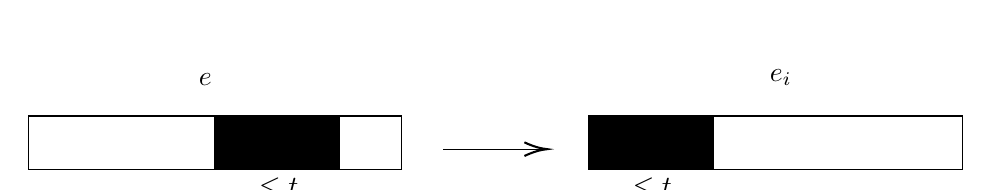
\begin{tikzpicture}[x=0.75pt,y=0.75pt,yscale=-1,xscale=1]
%uncomment if require: \path (0,334); %set diagram left start at 0, and has height of 334

%Flowchart: Process [id:dp6054046162100231] 
\draw   (60,104) -- (240,104) -- (240,130) -- (60,130) -- cycle ;
%Flowchart: Process [id:dp9632585876246007] 
\draw   (330,104) -- (510,104) -- (510,130) -- (330,130) -- cycle ;
%Flowchart: Process [id:dp6324300003108108] 
\draw  [fill={rgb, 255:red, 0; green, 0; blue, 0 }  ,fill opacity=1 ] (150,104) -- (210,104) -- (210,130) -- (150,130) -- cycle ;
%Flowchart: Process [id:dp5886209973046079] 
\draw  [fill={rgb, 255:red, 0; green, 0; blue, 0 }  ,fill opacity=1 ] (330,104) -- (390,104) -- (390,130) -- (330,130) -- cycle ;
%Straight Lines [id:da6331476223609735] 
\draw    (260,120) -- (308,120) ;
\draw [shift={(310,120)}, rotate = 180] [color={rgb, 255:red, 0; green, 0; blue, 0 }  ][line width=0.75]    (10.93,-3.29) .. controls (6.95,-1.4) and (3.31,-0.3) .. (0,0) .. controls (3.31,0.3) and (6.95,1.4) .. (10.93,3.29)   ;

% Text Node
\draw (141,82.4) node [anchor=north west][inner sep=0.75pt]    {$e$};
% Text Node
\draw (416,80.4) node [anchor=north west][inner sep=0.75pt]    {$e_{i}$};
% Text Node
\draw (170,132.4) node [anchor=north west][inner sep=0.75pt]    {$\leq t$};
% Text Node
\draw (350,132.4) node [anchor=north west][inner sep=0.75pt]    {$\leq t$};

\end{tikzpicture}

\end{center}

Then $s_i = He_i^T$ is a vector of length $n-k$ 
and has (non-cyclic) burst length $\leq t$. It follows that $e_i = (s_i, 0)$ and 
hence $e = x^{n-i}e_i$. 

Let $r = c+e$ so that $x^i r - x^i e = x^i c$. Note that $C$ is a cyclic code, so 
$x^i c$ is also a codeword, and hence $x^i r$ and $x^i e$ have the same syndrome. 
Therefore, in order to compute the syndromes of the cyclic shifts of the error vectors 
$s_i = He_i^T$, it suffices to compute the syndromes of $r_i = x^i r$ for all $0 \leq i \leq n-1$. 

\begin{algo}[Error-trapping decoding algorithm for cyclic burst error correcting codes]
Let $r(x)$ be the received word, and let $s_i(x)$ denote the syndrome of 
$x^ir(x)$ for each $0 \leq i \leq n-1$. 

\begin{algorithm}[H]
\begin{algorithmic}[1]
\FOR{$i=0$ to $n-1$}
\STATE Compute $s_i(x)$ \\
\IF{$s_i$ has (non-cyclic) burst length $\leq t$}
\STATE Let $e(x) = x^{n-i}(s_i, 0)$ \\
\STATE Decode $r(x)$ to $c(x) = r(x) - e(x)$
\ENDIF
\ENDFOR
\STATE Reject $r$
\end{algorithmic}
\end{algorithm}
\end{algo}

If the error vector is in fact a cyclic burst of length $\leq t$, then the algorithm will 
make the correct decision. 

\begin{exmp}
Recall that the $(15, 9)$-binary cyclic code with generator polynomial $g(x) 
= 1+x+x^2+x^3+x^6$ is a $3$-cyclic burst error correcting code. Decode the received word 
$r = 1110\,1110\,1100\,000$. 
\end{exmp}

{\sc Solution.} We begin by computing the syndromes of $r$ and its cyclic shifts. 

\begin{table}[H]
\centering
\begin{tabular}{c|c}
$i$ & $s_i(x)$ \\ \hline
0   & 110011   \\
1   & 100101   \\
2   & 101110   \\
3   & 010111   \\
4   & 110111   \\
5   & 100111   \\
6   & 101111   \\
7   & 101011   \\
8   & 101001   \\
9   & 101000  
\end{tabular}
\end{table}

Since $s_9$ has burst length $\leq 3$, we let $e(x) = x^{15-9} s_9(x) = 
x^6(1+x^2) = 0000\,0010\,1000\,000$, and we decode $r$ to 
$c = r- e = 1110\,1100\,0100\,000$. 

{\bf Interleaving.} Suppose we want to increase the cyclic burst error correcting capability of a code. 
Let $C$ be an $(n, k)$-code with cyclic burst error correcting capability $t$. Suppose that 
\begin{align*}
    c_1 &= (c_{11}, c_{12}, \dots, c_{1n}) \in C, \\
    c_2 &= (c_{21}, c_{22}, \dots, c_{2n}) \in C, \\
    & \qquad\qquad\quad \vdots \\
    c_s &= (c_{s1}, c_{s2}, \dots, c_{sn}) \in C.
\end{align*}
Instead of transmitting $c_1, c_2, \dots, c_s$ in that order, we transmit 
\[ c^* = (c_{11}, c_{21}, \dots, c_{s1}, c_{12}, c_{22}, \dots, c_{s2}, \dots, c_{1n}, c_{2n}, 
\dots, c_{sn}), \]
which are the columns of the above array. Then any cyclic burst of length $\leq st$ in 
$c^*$ results in a cyclic burst of length $\leq t$ in each of the original codewords 
$c_1, c_2, \dots, c_s$, which can then be corrected with the error-trapping algorithm. 
This is called {\bf interleaving to a depth of $s$}. 

\begin{thm}[Interleaving codes]
Let $C$ be an $(n, k)$-code over $F$ with cyclic burst error correcting capability $t$. 
Let $C^*$ be the code obtained by interleaving $C$ to a depth of $s$. 
\begin{enumerate}[(1)]
    \item $C^*$ is an $(ns, ks)$-code over $F$ with cyclic burst error correcting capability $ts$. 
    \item If $C$ is cyclic with generator polynomial $g(x)$, then $C^*$ is cyclic with 
    generator polynomial $g(x^s)$. 
\end{enumerate}
\end{thm}
\begin{pf}
We leave this as an exercise. For (1), show that $C^*$ is linear with length $ns$, dimension $ks$, and 
cyclic burst error correcting capability $ts$. For (2), prove that $g(x^s)$ is a monic 
divisor of $x^{ns}-1$ of degree $ns-ks$, and that $g(x^s) \mid c(x)$ for all $c \in C^*$. 
\end{pf}

\newpage 
\section{BCH codes}

In this section, we will be studying a special class of cyclic codes called BCH codes. Before we get 
to that, we will need some more field theory.

\subsection{Minimal polynomials}
Recall that if $F = \GF(p^m)$ is a finite field of characteristic $p$, then $\Z_p$ is a 
subfield of $F$, and we can view $F$ as an $m$-dimensional vector space over $\Z_p$. 

More generally, for any prime power $q$, we have that $\GF(q)$ is a subfield of $\GF(q^m)$, 
and we can view $\GF(q^m)$ has an $m$-dimensional vector space over $\GF(q)$. We call 
$\GF(q^m)$ an {\bf extension field} of $\GF(q)$. 

\begin{defn}
Let $\alpha \in \GF(q^m)$. The {\bf minimal polynomial of $\alpha$ over $\GF(q)$}, denoted by 
$m_\alpha(y)$, is the monic polynomial of smallest degree in $\GF(q)[y]$ that has 
$\alpha$ as a root. 
\end{defn}

\begin{remark}~
\begin{enumerate}[(1)]
    \item If $m(y) \in \GF(q)[y]$ is a non-zero polynomial with $m(\alpha) = 0$ and 
    $c$ is the leading coefficient of $m(y)$, then $\hat m(y) = c^{-1}m(y)$ is a monic polynomial 
    in $\GF(q)[y]$ with $\hat m(\alpha) = 0$. More generally, multiplying a polynomial 
    by a non-zero constant does not change the roots of the polynomial. 
    \item We have $m_0(y) = y$. 
    \item Suppose that $\alpha \neq 0$ and let $t$ be the order of $\alpha$. Recall that 
    $t \mid q^m - 1$. Then $\alpha$ is a root of the polynomial 
    $y^t - 1 \in \GF(q)[y]$. Hence, there always exists a monic polynomial of smallest 
    degree in $\GF(q)[y]$ having $\alpha$ as a root. 
\end{enumerate}
\end{remark}

\begin{exmp}
The minimal polynomials over $\GF(2)$ of the elements in $\GF(2^2) = \Z_2[x]/(x^2+x+1) 
= \{0, 1, x, x+1\}$ are 
\begin{align*}
    m_0(y) &= y, \\
    m_1(y) &= y+1, \\
    m_x(y) &= y^2 + y + 1, \\
    m_{x+1}(y) &= y^2 + y + 1. 
\end{align*}
\end{exmp}

\begin{thm}
Let $\alpha \in \GF(q^m)$. 
\begin{enumerate}[(a)]
    \item The minimal polynomial $m_\alpha(y)$ of $\alpha$ over $\GF(q)$ is unique.
    \item The minimal polynomial $m_\alpha(y)$ is irreducible over $\GF(q)$.
    \item We have $\deg(m_\alpha) \leq m$.
    \item If $f(y) \in \GF(q)[y]$, then $f(\alpha) = 0$ if and only if $m_\alpha(y) \mid f(y)$. 
\end{enumerate}
\end{thm}
\begin{pf}~
\begin{enumerate}[(a)]
    \item Suppose that $m_1(y), m_2(y) \in \GF(q)[y]$ are two monic polynomials of (the same)
    smallest degree with $m_1(\alpha) = m_2(\alpha) = 0$. Consider $r(y) = m_1(y) - m_2(y)$. Then 
    $r(\alpha) = m_1(\alpha) - m_2(\alpha) = 0 - 0 = 0$. But $\deg(r) < \deg(m_1)$ 
    as $m_1(y)$ and $m_2(y)$ are both monic, so we must have $r(y) = 0$. Therefore, 
    we obtain $m_1(y) = m_2(y)$. 
    \item Suppose towards a contradiction that $m_\alpha(y)$ is reducible over $\GF(q)$. 
    Then we can write $m_\alpha(y) = s(y)t(y)$ where $s(y), t(y) \in \GF(q)[y]$ with 
    $\deg(s), \deg(t) \leq \deg(m_\alpha)$. Then $m_\alpha(\alpha) = s(\alpha)t(\alpha) = 0$, 
    so we either have $s(\alpha) = 0$ or $t(\alpha) = 0$. In either case, this contradicts the 
    minimality of $\deg(m_\alpha)$, so $m_\alpha(y)$ must be irreducible over $\GF(q)$. 
    \item Recall that $\GF(q^m)$ is an $m$-dimensional vector space over $\GF(q)$. 
    Hence, the elements $1, \alpha, \alpha^2, \dots, \alpha^m$ are linearly dependent 
    over $\GF(q)$. In particular, we can write 
    \[ a_0 + a_1\alpha + a_2 \alpha^2 + \cdots + a_m \alpha^m = 0 \]
    for some $a_0, a_1, \dots, a_m \in \GF(q)$ which are not all zero. Then $\alpha$ is a 
    root of the non-zero polynomial 
    \[ m(y) = a_0 + a_1 y + \cdots + a_m y^m \in \GF(q)[y], \]
    so it follows that $\deg(m_\alpha) \leq m$. 
    \item Let $f(y) \in \GF(q)[y]$. By the division algorithm for polynomials, we can write 
    $f(y) = \ell(y) m_\alpha(y) + r(y)$ where $\ell(y), r(y) \in \GF(q)[y]$ and 
    $\deg(r) < \deg(m_\alpha)$. Now, we have $f(\alpha) = \ell(\alpha) m_\alpha(\alpha) + r(\alpha) 
    = r(\alpha)$, so we have 
    \begin{align*}
        f(\alpha) = 0 &\iff r(\alpha) = 0 \\
        &\iff r(y) = 0 \text{ (since $\deg(r) < \deg(m_\alpha)$)} \\
        &\iff m_\alpha(y) \mid f(y). \qedhere 
    \end{align*}
\end{enumerate}
\end{pf}

\subsection{Computing minimal polynomials}

We will show that the roots of the minimal polynomial $m_\alpha(y)$ of 
$\alpha$ over $\GF(q)$ are precisely the "conjugates" of $\alpha$ over $\GF(q)$. 
We first prove the following result. 

\begin{thm}
Let $\alpha \in \GF(q^m)$. Then $\alpha \in \GF(q)$ if and only if $\alpha^q = \alpha$.
\end{thm}
\begin{pf}
Since $\beta^q = \beta$ for all $\beta \in \GF(q)$, the elements of $\GF(q)$ are 
all roots of the polynomial $y^q - y \in \GF(q^m)[y]$. Since this polynomial 
has degree $q$, these $q$ elements are in fact the only roots. Thus, we have 
$\alpha \in \GF(q)$ if and only if $\alpha^q = \alpha$. 
\end{pf}

\begin{defn}
Let $\alpha \in \GF(q^m)$. Let $t$ be the smallest positive integer such that $\alpha^{q^t} = 
\alpha$ (and note that $t \leq m$). Then the {\bf set of conjugates with respect to 
$\GF(q)$} is 
\[ C(\alpha) := \{\alpha, \alpha^q, \alpha^{q^2}, \dots, \alpha^{q^{t-1}}\}. \]
Note that the elements of $C(\alpha)$ are distinct. 
\end{defn}

\begin{thm}
Let $\alpha \in \GF(q^m)$. The minimal polynomial of $\alpha$ over $\GF(q)$ is given by 
\[ m(y) = \prod_{\beta \in C(\alpha)} (y - \beta) = (y-\alpha)(y-\alpha^q)(y - \alpha^{q^2})
\cdots (y-\alpha^{q^{t-1}}). \]
\end{thm}
\begin{pf}
Clearly, $m(y)$ is monic and has $\alpha$ as a root. Now, write 
$m(y) = \sum_{i=0}^t m_i y^i \in \GF(q^m)[y]$. In order to show that $m(y) \in \GF(q)[y]$, 
we need to verify that $m_i \in \GF(q)$ for all $0 \leq i \leq t$. Indeed, note that 
\[ m(y)^q = \prod_{\beta \in C(\alpha)} (y-\beta)^q = \prod_{\beta \in C(\alpha)} 
(y^q - \beta^q) = \prod_{\beta \in C(\alpha)} (y^q - \beta) 
= m(y^q) = \sum_{i=0}^t m_i y^{iq}, \tag{1} \]
where the third equality follows from the fact that $C(\alpha) = \{\beta^q : \beta \in C(\alpha)\}$. 
Moreover, we have 
\[ m(y)^q = \left( \sum_{i=0}^t m_i y^i \right)^q = \sum_{i=0}^t m_i^q y^{iq}. \tag{2} \]
Comparing the coefficients of the $y^{iq}$ in (1) and (2) gives $m_i = m_i^q$ for all 
$0 \leq i \leq t$. By Theorem 6.2.1, we get $m_i \in \GF(q)$ for all $0 \leq i \leq t$, so 
$m(y) \in \GF(q)[y]$. Finally, suppose that $f(y) \in \GF(q)[y]$ is a non-zero polynomial 
such that $f(\alpha) = 0$. Write $f(y) = \sum_{i=0}^d f_i y^i$. Then 
\[ f(\alpha^q) = \sum_{i=0}^d f_i \alpha^{iq} = \left( \sum_{i=0}^d f_i \alpha^i \right)^q 
= f(\alpha)^q = 0, \]
so $\alpha, \alpha^q, \dots, \alpha^{q^{t-1}}$ are all roots of $f(y)$, which implies that 
$\deg(f) \geq t = \deg(m)$. Hence, $m(y)$ is the monic polynomial of smallest degree 
in $\GF(q)[y]$ that has $\alpha$ as a root. 
\end{pf}

\begin{exmp}
Let $\GF(2^4) = \Z_2[x]/(x^4+x+1)$. Find the minimal polynomial of $\beta = x^2 + x^3$ over 
$\Z_2$. 

{\sc Solution.} When doing computations by hand, it is useful to have a generator $\alpha$ 
of $\GF(2^4)^*$ and a table of powers of $\alpha$. It turns out that $\alpha = x$ is a 
generator of $\GF(2^4)^*$ with $\beta = \alpha^6$; see the $\GF(16)$ handout for the rest of 
the powers of $\alpha$. Then we get $C(\beta) = \{\alpha^6, \alpha^{12}, \alpha^9, 
\alpha^3\}$ where $\alpha^9 = \alpha^{24}$ and $\alpha^3 = \alpha^{48}$. 
By Theorem 6.2.3, it follows that 
\begin{align*}
    m_\beta(y) 
    &= (y - \alpha^3)(y - \alpha^6)(y-\alpha^9)(y-\alpha^{12}) \\
    &= [y^2 - (\alpha^3+\alpha^6)y + \alpha^9][y^2 - (\alpha^9 + \alpha^{12})y + \alpha^{21}] \\
    &= (y^2 + \alpha^2y + \alpha^9)(y^2 + \alpha^8y + \alpha^6) \\
    &= y^4 + (\alpha^2 + \alpha^8)y^3 + (\alpha^9 + \alpha^{10} + \alpha^6) y^2 
    + (\alpha^8 + \alpha^2)y + 1 \\
    &= y^4 + y^3 + y^2 + y + 1
\end{align*}
is the minimal polynomial of $\beta$ over $\Z_2$. 
\end{exmp}

\subsection{Factoring $x^n-1$ over $\GF(q)$ [Part 1]}

Our goal is to describe the complete factorization of $x^n - 1$ 
over $\GF(q)$. 
In doing so, we will see how generator polynomials $g(x)$ can be selected so that we have a 
useful lower bound on the distance of the cyclic code generated by $g(x)$. Such codes are known 
as {\bf BCH codes}. 

Let $p$ be the characteristic of $\GF(q)$. If $\gcd(n, q) \neq 1$, then we can write $n = n'p^\ell$ 
where $\ell \geq 1$ and $\gcd(n', p) = 1$. Then we have 
\[ x^n - 1 = (x^{n'} - 1)^{p^\ell}. \] 
In particular, we may assume without loss of generality that $\gcd(n, q) = 1$. 

We now introduce some notation. 
\begin{itemize}
    \item Let $m$ be the smallest positive integer such that $q^m \equiv 1 \text{ (mod $n$)}$. 
    \item Let $\alpha$ be a generator of $\GF(q^m)^*$. 
    \item Let $\beta = \alpha^{(q^m-1)/n}$. 
\end{itemize}
Note that $\beta \in \GF(q^m)$ with $\ord(\beta) = n$, and the elements 
$1, \beta, \beta^2, \dots, \beta^{n-1}$ are distinct. Moreover, for all $0 \leq i \leq n-1$, we have 
\[ (\beta^i)^n = (\beta^n)^i = 1^i = 1. \]
Hence, the elements $1, \beta, \beta^2, \dots, \beta^{n-1}$ are roots of $x^n-1$, and they are in fact 
the only roots as $x^n-1$ has degree $n$. Therefore, we see that 
\[ x^n - 1 = (x-1)(x-\beta)(x-\beta^2) \cdots (x-\beta^{n-1}) \]
is the complete factorization of $x^n-1$ over $\GF(q^m)$. However, we are seeking the 
complete factorization of 
$x^n - 1$ over $\GF(q)$, not $\GF(q^m)$. 

Consider $\beta^i$ where $0 \leq i \leq n-1$. Since $\beta^i$ is a root of $x^n-1$, we have 
$m_{\beta^i}(x) \mid x^n - 1$. Furthermore, the roots of $m_{\beta^i}(x)$ are 
\[ C(\beta^i) = \{\beta^i, \beta^{iq}, \beta^{iq^2}, \dots, \beta^{iq^{t-1}}\} \]
where $t$ is the smallest positive integer such that $iq^t \equiv i \text{ (mod $n$)}$. 

The above discussion motivates the following definition. 

\begin{defn}
Suppose that $\gcd(n, q) = 1$, and let $0 \leq i \leq n-1$. The {\bf cyclotomic coset of $q$ 
modulo $n$ containing $i$} is the set
\[ C_i = \{i, iq \text{ (mod $n$)}, iq^2 \text{ (mod $n$)}, \dots, iq^{t-1} \text{ (mod $n$)}\}, \]
where $t$ is the smallest positive integer such that $iq^t \equiv i \text{ (mod $n$)}$. 
Moreover, we define 
\[ C = \{C_i : 0 \leq i \leq n-1\} \]
to be the {\bf set of cyclotomic cosets of $q$ modulo $n$}. 
\end{defn}

\begin{exmp}
The cyclotomic cosets of $q = 2$ modulo $n = 15$ are 
\begin{align*}
    C_0 &= \{0\}, \\
    C_1 &= \{1, 2, 4, 8\} = C_2 = C_4 = C_8, \\
    C_2 &= \{3, 6, 12, 9\} = C_6 = C_{12} = C_9, \\
    C_5 &= \{5, 10\} = C_{10}, \\
    C_7 &= \{7, 14, 13, 11\} = C_{14} = C_{13} = C_{11}.
\end{align*}
Therefore, we have $C = \{C_0, C_1, C_3, C_5, C_7\}$. 
\end{exmp}

Note that if $j \in C_i$, then $C_j = C_i$, as the above example shows. Moreover, observe that 
\[ m_{\beta^i}(x) = (x-\beta^i)(x-\beta^{iq})(x-\beta^{iq^2}) \cdots (x-\beta^{iq^{t-1}}) = 
\prod_{j \in C_i} (x- \beta^j) \]
is an irreducible factor of $x^n-1$ over $\GF(q)$ of degree $|C_i|$. This leads to our main theorem. 

\begin{thm}
Suppose that $\gcd(n, q) = 1$.
\begin{enumerate}[(1)]
    \item The number of monic irreducible factors of $x^n-1$ over $\GF(q)$ is equal to the number 
    of (distinct) cyclotomic cosets of $q$ modulo $n$.
    \item The number of monic irreducible factors 
    of $x^n-1$ over $\GF(q)$ of degree $d$ is equal to the number of (distinct)
    cyclotomic cosets of $q$ modulo $n$ of size $d$. 
\end{enumerate}
\end{thm}

\subsection{Factoring $x^n-1$ over $\GF(q)$ [Part 2]}

\begin{thm}
Suppose that $\gcd(n, q) = 1$. Let $m$ be the smallest positive integer such that $q^m \equiv 1 
\text{ (mod $n$)}$, and let $\beta \in \GF(q^m)$ be an element of order $n$. Then the monic 
irreducible factors of $x^n-1$ over $\GF(q)$ are $\{m_{\beta^i}(x) : 0 \leq i \leq n-1\}$ where 
\[ m_{\beta^i}(x) = \prod_{j \in C_i} (x - \beta^j). \]
Note that if $j \in C_i$, then $m_{\beta^j}(x) = m_{\beta^i}(x)$. 
\end{thm}

\begin{exmp}
Factor $x^{15}-1$ over $\GF(2)$.

{\sc Solution.} In Example 6.3.2, we saw the cyclotomic cosets of $q = 2$ modulo $n = 15$. 
In particular, we know that $x^{15} - 1$ has five irreducible factors over $\GF(2)$; 
one factor has degree $1$, one factor has degree $2$, and three factors have degree $4$. Let 
us find these factors. 

The smallest positive integer $m$ such that $2^m \equiv 1 \text{ (mod $15$)}$ is $m=4$. 
We need an element $\beta \in \GF(q^m)$ of order $15$. From Example 6.2.4, we can take 
$\beta = \alpha$, where $\alpha$ is a generator of $\GF(2^4) = \Z_2[\alpha]/(\alpha^4+\alpha+1)$. 
Then, we obtain 
\begin{align*}
    m_{\beta^0}(x) &= 1+x, \\
    m_{\beta^1}(x) &= 1+x+x^4, \\
    m_{\beta^3}(x) &= 1+x+x^2+x^3+x^4, \\
    m_{\beta^5}(x) &= 1+x+x^2, \\
    m_{\beta^7}(x) &= 1+x^3+x^4.
\end{align*}
These can be computed in a similar fashion to Example 6.2.4; in fact, $m_{\beta^3}(x)$ was obtained 
from there. It follows that the complete factorization of $x^{15} - 1$ over $\GF(2)$ is 
\[ x^{15} - 1 = (1+x)(1+x+x^2)(1+x+x^4)(1+x^3+x^4)(1+x+x^2+x^3+x^4). \]
\end{exmp}

\begin{exmp}
Determine the number of cyclic subspaces of $V_{90}(\Z_3)$. 

{\sc Solution.} First, observe that $x^{90} - 1 = (x^{10} - 1)^9$. To determine the factorization 
pattern of $x^{10} - 1$ over $\Z_3$, we find the cyclotomic cosets of $q = 3$ modulo 
$n = 10$. Indeed, we have 
\begin{align*}
    C_0 &= \{0\}, \\
    C_1 &= \{1, 3, 9, 7\}, \\
    C_2 &= \{2, 4, 8, 6\}, \\
    C_5 &= \{5\}.
\end{align*}
Hence, it follows that $x^{90} - 1 = [f_0(x) \cdot f_1(x) \cdot f_2(x) \cdot f_5(x)]^9$ 
where $f_0(x), f_1(x), f_2(x), f_5(x) \in \Z_3[x]$ are irreducible over $\Z_3$ with 
$\deg(f_0) = \deg(f_5) = 1$ and $\deg(f_2) = \deg(f_3) = 4$. In particular, we have 
$f_i(x) = m_{\beta^i}(x)$ where $\beta \in \GF(3^4)$ has order $10$. Thus, the number of 
factors of $x^{90} - 1$ over $\Z_3$, which is equal to the number of cyclic subspaces of 
$V_{90}(\Z_3)$, is 
\[ (9+1)(9+1)(9+1)(9+1) = 10^4 = 10000. \]
\end{exmp}

\subsection{BCH codes}

BCH codes were discovered in 1960 by R. C. Bose and D. Ray-Chaudhuri, and independently in 
1959 by A. Hocquenghem. They are cyclic codes that are constructed in such a way that 
a useful lower bound on their distance is known. 

{\bf Setup.} Suppose that $\gcd(n, q) = 1$.
\begin{itemize}
    \item Let $m$ be the smallest positive integer such that $q^m \equiv 1 \text{ (mod $n$)}$. 
    \item Let $\alpha$ be a generator of $\GF(q^m)^*$, and let $\beta = \alpha^{(q^m-1)/n}$. 
    Recall that $\ord(\beta) = n$. 
    \item Let $m_{\beta^i}(x)$ denote the minimal polynomial of $\beta^i$ over $\GF(q)$ for all 
    $0 \leq i \leq n-1$, and recall that $m_{\beta^i}(x) \mid x^n - 1$. 
    \item For all $i \geq n$, we will set $m_{\beta^i}(x) = m_{\beta^j}(x)$ where 
    $j \equiv i \text{ (mod $n$)}$ with $0 \leq j \leq n-1$, 
    since $\beta^i = \beta^j$. 
\end{itemize}

\begin{defn}
A {\bf BCH code} $C$ over $\GF(q)$ of block length $n$ and designed distance $\delta$ is a cyclic 
code generated by the polynomial 
\[ g(x) = \lcm\{m_{\beta^i}(x) : a \leq i \leq a + \delta - 2\} \]
for some integer $a$. 
\end{defn}

\begin{remark}~
\begin{enumerate}[(1)]
    \item Since $m_{\beta^i}(x) \mid x^n-1$ for all $a \leq i \leq a+\delta-2$, it follows that 
    $g(x) \mid x^n-1$. Moreover, $g(x)$ is monic, so it is indeed the generator polynomial 
    of a cyclic code of length $n$ over $\GF(q)$. 
    \item The $\delta - 1$ consecutive powers of $\beta$, namely 
    $\beta^a, \beta^{a+1}, \dots, \beta^{a+\delta-2}$, are roots of $g(x)$. 
    \item The {\bf BCH bound} is given by $d(C) \geq \delta$, which we will prove in the following section.
\end{enumerate}
\end{remark}

\begin{exmp}
Let $q = 3$ and $n = 13$. Then $m = 13$ is the smallest positive integer such that $3^m \equiv 1 
\text{ (mod 13)}$. Consider $\GF(3^3) = \Z_3[\alpha]/(\alpha^3+2\alpha^2+1)$. Then 
$\alpha$ is a generator of $\GF(3^3)^*$ (see the $\GF(27)$ handout). Moreover, $\beta = \alpha^2$ 
is an element of order $13$. The cyclotomic cosets of $q = 3$ modulo $n = 13$ are 
\begin{align*}
    C_0 &= \{0\}, \\
    C_1 &= \{1, 3, 9\}, \\
    C_2 &= \{2, 6, 5\}, \\
    C_4 &= \{4, 12, 10\}, \\
    C_7 &= \{7, 8, 11\}. 
\end{align*}
It follows that 
\begin{align*}
    m_{\beta^0}(x) &= x+2, \\
    m_{\beta^1}(x) &= x^3 + 2x^2 + 2x + 2, \\
    m_{\beta^2}(x) &= x^3 + 2x + 2, \\
    m_{\beta^4}(x) &= x^3 + x^2 + x + 2, \\
    m_{\beta^7}(x) &= x^3 + 2x + 1.
\end{align*}
Now, let 
\[ g(x) = m_{\beta^0}(x) \cdot m_{\beta^1}(x) \cdot m_{\beta^2}(x) = 2 + 2x + x^4 + 2x^5 + x^6 + x^7. \] 
The roots of $g(x)$ are $\beta^0, \beta^1, \beta^3, \beta^9, \beta^2, \beta^6, \beta^5$. 
Since $\beta^0, \beta^1, \beta^2, \beta^3$ are among these roots, then by taking $a = 0$, 
we see that $g(x)$ generates a $(13, 6)$-BCH code over $\GF(3)$ with designed distance $\delta = 5$. 
By the BCH bound, the distance of this code is at least $5$. 
\end{exmp}

\begin{exercise}
Show that the polynomial $g(x) = m_{\beta^0}(x) \cdot m_{\beta^4}(x) \cdot m_{\beta^7}(x)$ generates a 
$(13, 6)$-BCH code over $\GF(3)$ of distance at least $5$. 
\end{exercise}

\subsection{BCH bound}

At the end of Section 1, we asked if there exists a block code with parameters $q = 2$, 
$n = 128$, $M = 2^{64}$, and $d \geq 22$. We can equivalently pose this as a sphere packing problem; 
namely, can we place $M = 2^{64}$ spheres of radius $e = \lfloor (d-1)/2 \rfloor \geq 10$ 
in $V_{128}(\Z_2)$ so that no two spheres overlap?

The answer is yes! We will describe an {\bf extended BCH code} with these parameters. 
First, we will describe a BCH code with parameters $q = 2$, $n = 127$, $k = 64$, and $\delta = 21$. 

The smallest integer $m$ such that $2^m \equiv 1 \text{ (mod 127)}$ is $m = 7$. The first 
few cyclotomic cosets of $2$ modulo $127$ are given by 
\begin{align*}
    C_0 &= \{0\}, \\
    C_1 &= \{\mathbf 1, \mathbf 2, \mathbf{4}, \mathbf{8}, \mathbf{16}, 32, 64\}, \\
    C_3 &= \{\mathbf 3, \mathbf 6, \mathbf{12}, 24, 48, 96, 65\}, \\
    C_5 &= \{\mathbf 5, \mathbf{10}, \mathbf{20}, 40, 80, 33, 66\}, \\
    C_7 &= \{\mathbf 7, \mathbf{14}, 28, 56, 112, 97, 67\}, \\
    C_9 &= \{\mathbf 9, \mathbf{18}, 36, 72, \mathbf{17}, 34, 68\}, \\
    C_{11} &= \{\mathbf{11}, 22, 44, 88, 49, 98, 69\}, \\
    C_{13} &= \{\mathbf{13}, 26, 52, 104, 81, 35, 70\}, \\
    C_{15} &= \{\mathbf{15}, 30, 60, 120, 113, 99, 71\}, \\
    C_{19} &= \{\mathbf{19}, 38, 76, 25, 50, 100, 73\}. 
\end{align*}
Let $\beta$ be an element of order $127$ in $\GF(2^7)^*$. Then the polynomial
\begin{align*}
    g(x) = m_{\beta^1}(x) \cdot m_{\beta^3}(x) \cdot m_{\beta^5}(x) \cdot m_{\beta^7}(x) \cdot m_{\beta^9}(x) \cdot m_{\beta^{11}}(x) \cdot m_{\beta^{13}}(x) \cdot m_{\beta^{15}}(x) \cdot m_{\beta^{19}}(x) 
\end{align*}
is a degree $63$ divisor of $x^{127} - 1$ over $\GF(2)$. Moreover, $\beta^i$ is a root of 
$g(x)$ for all $1 \leq i \leq 20$, so $g(x)$ generates a $(127, 64)$-binary BCH code $C$ with 
designed distance $\delta = 21$. 
Finally, the extended code of $C$, obtained by adding a parity bit to each codeword in $C$, 
is a $(128, 64)$-binary code with distance $\geq 22$. 

\begin{defn}
A {\bf Vandermonde matrix} over a field $F$ is a matrix of the form 
\[ A(x_1, x_2, \dots, x_t) = \begin{bmatrix} 1 & 1 & \cdots & 1 \\ 
x_1 & x_2 & \cdots & x_t \\ 
x_1^2 & x_2^2 & \cdots & x_t^2 \\
\vdots & \vdots & \ddots & \vdots \\
x_1^{t-1} & x_2^{t-1} & \cdots & x_t^{t-1} \end{bmatrix}_{t\times t} \]
where $x_1, x_2, \dots, x_t \in F$. 
\end{defn}

\begin{thm}
A Vandermonde matrix $A(x_1, x_2, \dots, x_t)$ over $F$ is non-singular if and only if the elements 
$x_1, x_2, \dots, x_t \in F$ are distinct. 
\end{thm}
\begin{pf}
Perform the row operations 
\begin{align*}
    R_t &\gets R_t - x_1R_{t-1} \\ 
    R_{t-1} &\gets R_{t-1} - x_1R_{t-2} \\
    &\qquad\;\; \vdots \\ 
    R_2 &\gets R_2 - x_1R_1
\end{align*}
to $A$ to obtain the matrix 
\[ A_1 = \begin{bmatrix}
1 & 1 & 1 & \cdots & 1 \\
0 & x_2-x_1 & x_3-x_1 & \cdots & x_t-x_1 \\
0 & x_2^2-x_1x_1 & x_3^2-x_1x_3 & \cdots & x_t^2-x_1x_t \\
\vdots & \vdots & \vdots & \ddots & \vdots \\ 
0 & x_2^{t-1}-x_1x_2^{t-1} & x_3^{t-1}-x_1x_3^{t-2} & \cdots & x_t^{t-1}-x_1x_t^{t-2} 
\end{bmatrix}. \]
Now, we can compute $\det(A_1)$ by expanding along the first column to get 
\[ \det(A) = \det(A_1) = (x_2-x_1)(x_3-x_1)\cdots(x_t-x_1) \cdot 
\det \begin{bmatrix}
1 & 1 & \cdots & 1 \\ 
x_2 & x_3 & \cdots & x_t \\
x_2^2 & x_3^2 & \cdots & x_t^2 \\
\vdots & \vdots & \ddots & \vdots \\
x_2^{t-2} & x_3^{t-2} & \cdots & x_t^{t-2} 
\end{bmatrix}. \]
By induction, it follows that 
\[ \det(A) = \prod_{1 \leq i < j \leq t} (x_j - x_i). \]
In particular, we have $\det(A) \neq 0$ if and only if the elements $x_1, x_2, \dots, x_t \in F$ 
are distinct. 
\end{pf}

\begin{thm}[BCH bound]
Let $C$ be an $(n, k)$-BCH code over $\GF(q)$ with designed distance $\delta$. Then $d(C) \geq \delta$. 
\end{thm}
\begin{pf}
Let $g(x)$ be the generator polynomial for $C$. For simplicity, suppose $a = 1$ so that 
$\beta, \beta^2, \dots, \beta^{\delta-1}$ are the roots of $g(x)$ where 
$\beta \in \GF(q^m)$ is an element of order $n$ and $m$ is the smallest positive integer such that 
$q^m \equiv 1 \text{ (mod $n$)}$. That is, we have $g(x) = \lcm\{m_{\beta^i}(x) : 1 \leq i \leq \delta-1
\}$. Now, let $r \in V_n(\GF(q))$. Then 
\begin{align*}
    r \in C &\iff g(x) \mid r(x) \\
    &\iff m_{\beta^i}(x) \mid r(x) \text{ for all } 1 \leq i \leq \delta-1 \\
    &\iff r(\beta^i) = 0 \text{ for all } 1 \leq i \leq \delta-1. 
\end{align*}
Now, let 
\[ H_1 = \begin{bmatrix}
1 & \beta & \beta^2 & \cdots & \beta^{n-1} \\ 
1 & \beta^2 & (\beta^2)^2 & \cdots & (\beta^2)^{n-1} \\
1 & \beta^3 & (\beta^3)^2 & \cdots & (\beta^3)^{n-1} \\
\vdots & \vdots & \vdots & \ddots & \vdots \\
1 & \beta^{\delta-1} & (\beta^{\delta-1})^2 & \cdots & (\beta^{\delta-1})^{n-1} 
\end{bmatrix}_{(\delta-1)\times n}. \]
Note that $r \in C$ if and only if $H_1r^T = 0$. Moreover, no $t = \delta-1$ columns of $H_1$ are 
linearly dependent over $\GF(q^m)$. Indeed, we have 
\begin{align*} \det \begin{bmatrix}
\beta^{i_1} & \beta^{i_2} & \cdots & \beta^{i_t} \\
(\beta^2)^{i_1} & (\beta^2)^{i_2} & \cdots & (\beta^2)^{i_t} \\
\vdots & \vdots & \ddots & \vdots \\ 
(\beta^{\delta-1})^{i_1} & (\beta^{\delta-1})^{i_2} & \cdots & (\beta^{\delta-1})^{i_t}
\end{bmatrix}_{t\times t} 
&= \beta^{i_1}\beta^{i_2} \cdots \beta^{i_t} \cdot \det \begin{bmatrix}
1 & 1 & \cdots & 1 \\
\beta^{i_1} & \beta^{i_2} & \cdots & \beta^{i_t} \\
\vdots & \vdots & \ddots & \vdots \\
(\beta^{i_1})^{\delta-2} & (\beta^{i_2})^{\delta-2} & \cdots & (\beta^{i_t})^{\delta-2} 
\end{bmatrix} \\
&= \prod_{j=1}^t \beta^{i_j} \cdot \det(A(\beta^{i_1}, \beta^{i_2}, \dots, \beta^{i_t})) \neq 0,
\end{align*}
where the inequality follows from Theorem 6.6.2
as the elements $\beta^{i_1}, \beta^{i_2}, \dots, \beta^{i_t}$ are 
distinct. Since $\GF(q) \subseteq \GF(q^m)$, we also have that no $\delta-1$ columns of $H_1$ 
are linearly dependent over $\GF(q)$. 

Now, if $c \in C$ is a non-zero codeword with $w(c) < \delta$, then $H_1c^T = 0$ implies that we can write 
$0$ as a non-trivial linear combination of $\delta-1$ or fewer columns of $H_1$, contradicting what 
we just proved. Thus, every non-zero codeword in $C$ has weight $\geq \delta$, so 
$d(C) \geq \delta$. 
\end{pf}

\subsection{BCH decoding [Part 1]}

Over the years, many efficient algorithms have been designed for decoding BCH codes. For now, 
we will present a decoding algorithm for a specific BCH code called $C_{15}$. This decoding 
algorithm captures the essential ideas for a decoding algorithm for general BCH codes. 

First, we define the BCH code $C_{15}$. Let $\GF(2^4) = \Z_2[\alpha]/(\alpha^4 + \alpha + 1)$. 
Then $\alpha$ is a generator of $\GF(2^4)^*$, and $\beta = \alpha$ has order $15$. Define the polynomial 
\[ g(x) = m_\beta(x) \cdot m_{\beta^3}(x) = (x^4+x+1)(x^4+x^3+x^2+x+1) = 1+x^4+x^6+x^7+x^8. \]
The roots of $g(x)$ include $\beta, \beta^2, \beta^3, \beta^4$, so $g(x)$ generates a 
$(15, 7)$-BCH code over $\Z_2$ with designed distance $\delta = 5$, which we call $C_{15}$. 
In fact, since $g(x)$ is a codeword of weight $5$, we have $d(C_{15}) = 5$. Note that 
$C_{15}$ is a $2$-error correcting code. 

{\bf Parity-check matrix.} We now find a parity-check matrix for $C_{15}$. Let $r \in V_{15}(\Z_2)$. 
Then we have 
\begin{align*}
    r \in C_{15} &\iff g(x) \mid r(x) \\
    &\iff m_\beta(x) \mid r(x) \text{ and } m_{\beta^3}(x) \mid r(x) \\
    &\iff r(\beta) = 0 \text{ and } r(\beta^3) = 0. 
\end{align*}
Thus, a parity-check matrix for $C_{15}$ is given by 
\[ H = \begin{bmatrix} \beta^0 & \beta^1 & \beta^2 & \cdots & \beta^{14} \\ 
(\beta^3)^0 & (\beta^3)^1 & (\beta^3)^2 & \cdots & (\beta^3)^{14} \end{bmatrix}_{8 \times 15}. \]
Note that $H$ is a $2 \times 15$ matrix over $\GF(2^4)$, and we can convert it into an 
$8 \times 15$ matrix over $\Z_2$ by replacing each element in the matrix by its vector 
representation over $\Z_2$. 

{\bf Syndromes.} The syndrome of $r \in V_{15}(\Z_2)$ is 
\[ Hr^T = \begin{bmatrix} r(\beta) \\ r(\beta^3) \end{bmatrix} =: \begin{bmatrix} s_1 \\ s_3 \end{bmatrix}. \]
In this case, we do not require the parity-check matrix $H$ to compute syndromes;
we only have to compute 
$s_1 = r(\beta)$ and $s_3 = r(\beta^3)$. 

{\bf Decoding strategy.} If there is an error vector $e$ of weight $\leq 2$ that has the 
same syndrome $(s_1, s_3)$ as $r$, then we decode $r$ to $c = r-e$. Otherwise, we reject $r$. 

\subsection{BCH decoding [Part 2]}

We now present a decoding algorithm for $C_{15}$ with justification. 
\begin{enumerate}[(1)]
    \item Let $r \in V_{15}(\Z_2)$ be the received word. 
    \item Compute $s_1 = r(\beta)$ and $s_3 = r(\beta^3)$. 
    \item If $s_1 = s_3 = 0$, then accept $r$ and stop. 
    \item Suppose that $e(x) = x^i$; that is, exactly one error has occurred in position $i$, 
    where $0 \leq i \leq 14$. Then $s_1 = r(\beta) = e(\beta) = \beta^i$ and 
    $s_3 = r(\beta^3) = e(\beta^3) = \beta^{3i}$ so that $s_3 = s_1^3$. 
    
    If $s_1^3 = s_3$, then correct $r$ in position $i$ where $s_1 = \beta^i$, then stop. 
    \item If $r(\beta^3) = e(\beta^3) \neq 0$, we have $e(x) \neq 0$. Moreover, if 
    $s_1 = r(\beta) = 0$, then $e(\beta) = 0$ so that $m_\beta(x) \mid e(x)$. 
    Hence, we have $w(e) \geq 3$, since the BCH code generated by $m_\beta(x)$ has 
    designed distance $\delta \geq 3$. 
    
    If $s_1 = 0$ and $s_3 \neq 0$, then reject $r$ and stop. 
    \item If exactly two errors have occurred, say in positions $i$ and $j$ where 
    $0 \leq i \neq j \leq 14$, then $e(x) = x^i+x^j$. Then we have $s_1 = r(\beta) = 
    e(\beta) = \beta^i + \beta^j$ and 
    \begin{align*}
        s_3 = r(\beta^3) = e(\beta^3) 
        &= \beta^{3i} + \beta^{3j} \\
        &= (\beta^i + \beta^j)(\beta^{2i} + \beta^{i+j} + \beta^{2j}) \\
        &= (\beta^i + \beta^j)((\beta^i+\beta^j)^2 + \beta^{i+j}) \\
        &= s_1(s_1^2 + \beta^{i+j}). 
    \end{align*}
    In particular, we have $\beta^i+\beta^j = s_3/s_1 + s_1^2$, so $\beta^i$ and 
    $\beta^j$ are both roots of the polynomial 
    $z^2 + (\beta^i+\beta^j)z + \beta^{i+j} = z^2 + s_1z + (s_3/s_1 + s_1^2)$. 
    
    Form the {\bf error locator polynomial} 
    \[ \sigma(z) = z^2 + s_1z + \left( \frac{s_3}{s_1} + s_1^2 \right) \]
    and find its roots, if any, in $\GF(2^4)$. If there are two roots of $\sigma(z)$ given by $\beta^i$ 
    and $\beta^j$, then correct $r$ in positions $i$ and $j$, and stop. 
    \item Reject $r$. 
\end{enumerate}

We summarize our algorithm below. 

\begin{algo}~
\begin{enumerate}[(1)]
    \item Let $r \in V_{15}(\Z_2)$ be the received word. 
    \item Compute $s_1 = r(\beta)$ and $s_3 = r(\beta^3)$. 
    \item If $s_1 = s_3 = 0$, then accept $r$ and stop. 
    \item If $s_1^3 = s_3$, then correct $r$ in position $i$ where $s_1 = \beta^i$, then stop. 
    \item If $s_1 = 0$ and $s_3 \neq 0$, then reject $r$ and stop. 
    \item Form the {\bf error locator polynomial} 
    \[ \sigma(z) = z^2 + s_1z + \left( \frac{s_3}{s_1} + s_1^2 \right) \]
    and find its roots in $\GF(2^4)$. If there are two distinct roots of $\sigma(z)$ 
    given by $\beta^i$ and $\beta^j$, then correct $r$ in positions $i$ and $j$, and stop. 
    \item Reject $r$. 
\end{enumerate}
\end{algo}

This algorithm is guaranteed to make the correct decision if $w(e) \leq 2$. 

\begin{exmp}
Let $r = 10001\,00110\,00000 = 1 + x^4 + x^7 + x^8$ be the received word. Then we have 
\begin{align*}
    s_1 &= r(\beta) = 1 + \beta^4 + \beta^7 + \beta^8 = \beta + \beta^{11} = \beta^6, \\
    s_3 &= r(\beta^3) = 1 + \beta^{12} + \beta^6 + \beta^9 + \beta^3. 
\end{align*}
Observe that $s_1^3 = (\beta^6)^3 = \beta^{18} = \beta^3 = s_3$, so one error has occurred in 
position $6$. Thus, we decode $r$ to $c = 10001\,0\mathbf{1}110\,00000$. 
\end{exmp}

\begin{exmp}
Let $r = 00111\,01110\,00000 = x^2 + x^3 + x^4 + x^6 + x^7 + x^8$ be the received word. We have 
\begin{align*}
    s_1 &= r(\beta) = \beta^2 + \beta^3 + \beta^4 + \beta^6 + \beta^7 + \beta^8 = \beta^{13}, \\
    s_3 &= r(\beta^3) = \beta^6 + \beta^9 + \beta^{12} + \beta^3 + \beta^6 + \beta^9 = \beta^{10}. 
\end{align*}
Notice that $s_1^3 = \beta^{39} = \beta^9 \neq s_3$. Now, the error locator polynomial is given by 
\[ \sigma(z) = z^2 + s_1z + \left( \frac{s_3}{s_1} + s_1^2 \right) = 
z^2 + \beta^{13}z + (\beta^{12} + \beta^{11}) = z^2 + \beta^{13}z + 1. \]
Suppose that the roots of $\sigma(z)$ are $\beta^i$ and $\beta^j$. Then $\beta^i \cdot \beta^j 
= \beta^{i+j} = 1 = \beta^0$, so we see that $i + j \equiv 0 \text{ (mod 15)}$. Therefore, 
we check if $\beta^i + \beta^j = \beta^{13}$ for the pairs 
\[ (i, j) \in \{(1, 14), (2, 13), (3, 12), (4, 11), (5, 10), (6, 9), (7, 8)\}. \]
It turns out that $\beta^4 + \beta^{11} = \beta^{13}$, so two errors have occurred at positions $4$ 
and $11$. Finally, we decode $r$ to $c = 0011\mathbf{0}\,01110\,0\mathbf{1}000$. 
\end{exmp}

{\bf The general case.}
Suppose that $C$ is an $(n, k)$-BCH code over $\Z_2$ with designed distance $\delta$. Suppose the 
generator polynomial of $C$ is 
\[ g(x) = \lcm\{m_{\beta^i}(x) : 1 \leq i \leq \delta-1\}, \]
where $\beta \in \GF(2^m)$ has order $n$. Then we have $d(C) \geq \delta$. Let $t = \lfloor 
(\delta-1)/2 \rfloor$. 

Suppose that $c \in C$ is transmitted where $w(e) \leq t$, and $r$ is received. Compute 
$s_i = r(\beta^i)$ for all $1 \leq i \leq \delta-1$, and form the {\bf syndrome polynomial} 
\[ S(z) = s_1 + s_2z + s_3z^2 + \cdots + s_{\delta-1} z^{\delta-2}. \]
From the syndrome polynomial $S(z)$, the error locator polynomial $\sigma(z)$ can be efficiently 
computed. The roots of $\sigma(z)$ are given by $\beta^{-j}$, where $j$ denotes an error position. 

Moreover, this algorithm generalizes to BCH codes over $\GF(q)$.

\newpage 
\section{Reed-Solomon codes}

\counterwithin{thm}{section}

Reed-Solomon codes were invented by Irving Reed and Gustave Solomon in 1960. 

\begin{defn}
A {\bf Reed-Solomon (RS) code} is a BCH code of length $n$ over $\GF(q)$ such that $n \mid q-1$. 
\end{defn}

\begin{exmp}
Let $q = 2^4$ and consider $\GF(2^4) = \Z_2[\alpha]/(\alpha^4 + \alpha + 1)$. 
Recall that $\alpha$ is a generator of $\GF(2^4)^*$. Let $\beta = \alpha^3$, 
and note that $\ord(\beta) = 5$ (so that $n = 5$). Let 
\begin{align*}
    g(x) 
    &= \lcm \{m_\beta(x), m_{\beta^2}(x), m_{\beta^3}(x)\} \\
    &= (x-\beta)(x-\beta^2)(x-\beta^3) \\
    &= x^3 + \alpha^{11} x^2 + \alpha^2 x + \alpha^3. 
\end{align*}
Then $g(x)$ generates a $(5, 2)$-RS code $C$ over $\GF(2^4)$ with designed distance $\delta = 4$. 
In fact, we have $d(C) = 4$ since $g(x)$ is a codeword of weight $4$. A generator matrix for $C$ is 
given by 
\[ G = \begin{bmatrix}
\alpha^3 & \alpha^2 & \alpha^{11} & 1 & 0 \\ 0 & \alpha^3 & \alpha^2 & \alpha^{11} & 1
\end{bmatrix}_{2\times5}. \] 
Consider the code $C'$ obtained by $C$ by replacing each symbol in the codewords of $C$ 
by their binary vector representation. For instance, we set 
\[ (\alpha^3, \alpha^2, \alpha^{11}, 1, 0) \leftrightarrow (0001, 0010, 0111, 1000, 0000). \]
It is not difficult to see that $C'$ is closed under addition and scalar multiplication over 
$\Z_2$. Thus, $C'$ is a $(20, 8)$-binary code. 
\end{exmp}

More generally, suppose that $n \mid q-1$, and let $\beta \in \GF(q)$ be an element of order $n$. 
Then $m_{\beta^i}(x) = x - \beta^i$ for all $0 \leq i \leq n-1$. Hence, an RS code $C$ of length $n$ 
over $\GF(q)$ with designed distance $\delta$ is a BCH code over $\GF(q)$ with generator polynomial 
\[ g(x) = (x-\beta^a)(x-\beta^{a+1})(x - \beta^{a+2}) \cdots (x - \beta^{a+\delta-2}) \]
for some positive integer $a$. Since $\deg(g) = \delta - 1$, we have $w(g) \leq \delta$, so 
$d(C) \leq \delta$. On the other hand, the BCH bound gives $d(C) \geq \delta$, so $d(C) = \delta$. 

Moreover, since $\dim(C) = k = n-\deg(g) = n -\delta+1$, we have $k = n-d+1$, and rearranging
gives $d = n-k+1$. 
Recall that $d \leq n-k+1$ for any $(n, k, d)$-code. Thus, RS codes are optimal in the sense that 
they achieve maximum distance among all $(n, k)$-codes over $\GF(q)$ for any fixed $n$, $k$, and $q$. 

We note that RS codes have good cyclic burst error correcting capability. Indeed, let $C$ 
be an RS code of length $n$ over $\GF(2^4)$ with designed distance $\delta$. Consider any 
codeword $c = (c_1, \dots, c_n) \in C$, and note that each $c_i \in \GF(2^r)$. Let 
$e = \lfloor (d-1)/2 \rfloor = \lfloor (n-k)/2 \rfloor$. 

By identifying each $c_i$ as a binary vector of length $r$, we can view $c$ as a binary vector of 
length $nr$. Now, if $c$ is transmitted and a cyclic burst error of length $\leq 1 + (e-1)r$ is 
introduced, then at most $e$ $\GF(2^r)$-symbols of $c$ are received incorrectly. Thus, the 
received word can be decoded correctly.

\begin{thm}
Let $C$ be an $(n, k)$-RS code over $\GF(2^r)$. Let $C'$ be the code obtained by replacing 
each symbol in the codewords of $C$ by their $r$-bit binary representations. Then $C'$ 
is an $(nr, kr)$-binary code with cyclic burst error correcting capability 
$t = 1 + (\lfloor (n-k)/2 \rfloor - 1)r$. 
\end{thm}

\begin{exmp}
Consider $\GF(2^8) = \Z_2[\alpha]/(\alpha^8 + \alpha^4 + \alpha^3 + \alpha^2 + 1)$. Then 
$\beta = \alpha$ has order $255$ (so that $q = 256$ and $n = 255$). Let 
$g(x) = \prod_{i=1}^{24} (x-\beta^i)$.
Then $g(x)$ is the generator polynomial for a $(255, 231, 25)$-RS code $C$ with error 
correcting capability $e = 12$. The corresponding code $C'$ is then a $(2040, 1848)$-binary 
code with cyclic burst error correcting capability $t = 89$. 
This code $C$, and others derived from it, have been widely used in practice, such as in DVDs, 
CDs, and QR codes. 
\end{exmp}

\newpage 
\section{Code-based cryptography}

{\bf Public-key encryption.} The goal of public-key encryption is confidentiality when communicating 
over an insecured channel. The main feature of public-key encryption is that the two communicating 
parties do not share any secrets; they only share public information which has been 
authenticated. 

\begin{center}

\tikzset{every picture/.style={line width=0.75pt}} %set default line width to 0.75pt        

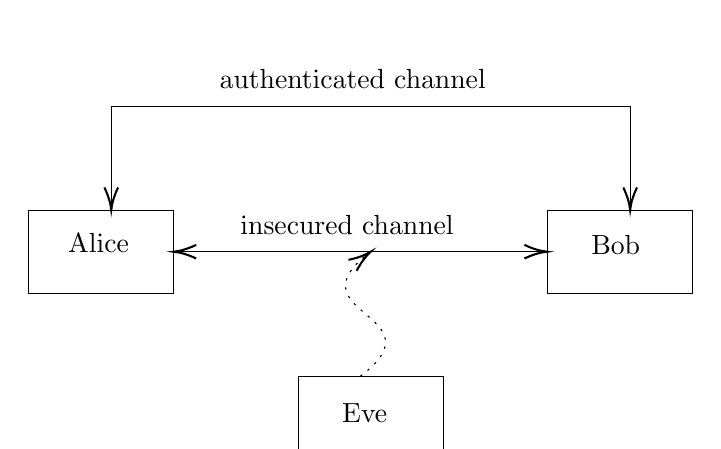
\begin{tikzpicture}[x=0.75pt,y=0.75pt,yscale=-1,xscale=1]
%uncomment if require: \path (0,334); %set diagram left start at 0, and has height of 334

%Shape: Rectangle [id:dp9852118809664145] 
\draw   (140,110) -- (210,110) -- (210,150) -- (140,150) -- cycle ;
%Shape: Rectangle [id:dp6717640262879949] 
\draw   (390,110) -- (460,110) -- (460,150) -- (390,150) -- cycle ;
%Straight Lines [id:da7888006824084179] 
\draw    (212,130) -- (388,130) ;
\draw [shift={(390,130)}, rotate = 180] [color={rgb, 255:red, 0; green, 0; blue, 0 }  ][line width=0.75]    (10.93,-3.29) .. controls (6.95,-1.4) and (3.31,-0.3) .. (0,0) .. controls (3.31,0.3) and (6.95,1.4) .. (10.93,3.29)   ;
\draw [shift={(210,130)}, rotate = 0] [color={rgb, 255:red, 0; green, 0; blue, 0 }  ][line width=0.75]    (10.93,-3.29) .. controls (6.95,-1.4) and (3.31,-0.3) .. (0,0) .. controls (3.31,0.3) and (6.95,1.4) .. (10.93,3.29)   ;
%Curve Lines [id:da8301628476827441] 
\draw  [dash pattern={on 0.84pt off 2.51pt}]  (300,190) .. controls (339.6,160.3) and (266.49,160) .. (303.83,130.89) ;
\draw [shift={(305,130)}, rotate = 503.13] [color={rgb, 255:red, 0; green, 0; blue, 0 }  ][line width=0.75]    (10.93,-3.29) .. controls (6.95,-1.4) and (3.31,-0.3) .. (0,0) .. controls (3.31,0.3) and (6.95,1.4) .. (10.93,3.29)   ;
%Shape: Rectangle [id:dp9544462783227079] 
\draw   (270,190) -- (340,190) -- (340,230) -- (270,230) -- cycle ;
%Straight Lines [id:da03146984771293271] 
\draw    (180,60) -- (430,60) ;
%Straight Lines [id:da33436360566117695] 
\draw    (430,60) -- (430,108) ;
\draw [shift={(430,110)}, rotate = 270] [color={rgb, 255:red, 0; green, 0; blue, 0 }  ][line width=0.75]    (10.93,-3.29) .. controls (6.95,-1.4) and (3.31,-0.3) .. (0,0) .. controls (3.31,0.3) and (6.95,1.4) .. (10.93,3.29)   ;
%Straight Lines [id:da39924490485950503] 
\draw    (180,60) -- (180,108) ;
\draw [shift={(180,110)}, rotate = 270] [color={rgb, 255:red, 0; green, 0; blue, 0 }  ][line width=0.75]    (10.93,-3.29) .. controls (6.95,-1.4) and (3.31,-0.3) .. (0,0) .. controls (3.31,0.3) and (6.95,1.4) .. (10.93,3.29)   ;

% Text Node
\draw (158,120) node [anchor=north west][inner sep=0.75pt]   [align=left] {Alice};
% Text Node
\draw (410,121) node [anchor=north west][inner sep=0.75pt]   [align=left] {Bob};
% Text Node
\draw (241,111) node [anchor=north west][inner sep=0.75pt]   [align=left] {insecured channel};
% Text Node
\draw (290,202) node [anchor=north west][inner sep=0.75pt]   [align=left] {Eve};
% Text Node
\draw (231,41) node [anchor=north west][inner sep=0.75pt]   [align=left] {authenticated channel};

\end{tikzpicture}

\end{center}

Recall the basic RSA encryption scheme, which was covered in MATH 135. 
\begin{itemize}
    \item {\bf Key generation.} Alice does the following: 
    \begin{enumerate}
        \item Randomlly select two large primes $p$ and $q$. 
        \item Compute $n = pq$ and $\Phi(n) = (p-1)(q-1)$. 
        \item Select an arbitrary $e$ such that $1 < e < \Phi(n)$ and $\gcd(e, \Phi(n)) = 1$. 
        \item Compute $d = e^{-1} \text{ (mod $\Phi(n)$)}$. 
        \item Alice's public key is $(n, e)$; her private key is $d$. 
    \end{enumerate}
    \item {\bf Encryption.} To encrypt the message to Alice, Bob does the following:
    \begin{enumerate}
        \item Obtain an authentic copy of Alice's public key $(n, e)$. 
        \item Represent the message $m$ as an integer from the interval $[0, n-1]$. 
        \item Compute $c = m^e \text{ (mod $n$)}$. 
        \item Send $c$ to Alice over the insecured channel. 
    \end{enumerate}
    \item {\bf Decryption.} To decrypt $c$, Alice simply computes $m = c^d \text{ (mod $n$)}$. 
\end{itemize}

{\bf The threat of quantum computers.} 
The security of the RSA encryption scheme is based on the hardness of factoring $n$. However, 
it has been known since 1994 that factoring $n$ is easy on a quantum computer. Elliptic 
curve cryptography, a widely used alternative to RSA, can also be broken easily by quantum computers. 
Fortunately, we are still far away from being able to build large-scale quantum computers. 
Nonetheless, it seems prudent to develop public-key encryption schemes that resist attacks even 
by quantum computers. 

{\bf McEliece public-key encryption scheme (1978).} The security of the McEliece public-key
encryption scheme is based on the fact that decoding a random (binary) linear code is 
{\bf NP}-hard. We give the basic idea in the next paragraph, and a high-level description of the 
encryption scheme following that. 

We first select a code $C$ for which an efficient decoding algorithm is known. 
We disguise $C$ to get a "random looking" code $\hat C$. The code $\hat C$ is the public key,
and the "disguising factor" is the private key. To encrypt the message, encode 
$m$ to obtain a codeword $\hat c \in \hat C$, add a random error $e$ to $\hat c$ to get 
$\hat r$, and send $\hat r$. Finally, to decrypt the message, use the "disguising factor" 
to convert the decoding problem into one for $C$, and use the decoding algorithm for $C$ 
to recover $e$ and $m$. 
\newpage 
\begin{itemize}
    \item {\bf Key generation.} Alice does the following: 
    \begin{enumerate}
        \item Select a $k \times n$ generator matrix $G$ for a $t$-error correcting binary Goppa code $C$.
        \item Select a random $k \times k$ invertible matrix $S$. 
        \item Select a random $n \times n$ permutation matrix $P$. 
        \item Compute $\hat G = SGP$, which will be a $k \times n$ matrix of rank $k$. 
        \item Alice's public key is $(\hat G, t)$; her private key is $(G, S, P)$. 
    \end{enumerate}
    It is conjectured that $\hat G$ is indistinguishable from a random $k \times n$ binary 
    matrix of rank $k$. 
    \item {\bf Encryption.} To encrypt a message for Alice, Bob does the following:
    \begin{enumerate}
        \item Obtain an authentic copy of Alice's public key $(\hat G, t)$. 
        \item Represent the message as a binary vector $m$ of length $k$. 
        \item Select a random binary vector $e \in V_n(\Z_2)$ of weight $t$. 
        \item Compute $\hat r = m\hat G + e$, and send $\hat r$ to Alice over the insecured channel.
    \end{enumerate}
    \item {\bf Decryption.} To decrypt $\hat r$, Alice does the following:
    \begin{enumerate}
        \item Compute $r = \hat r P^{-1}$. We note that 
        \[ r = \hat r P^{-1} = m \hat G P^{-1} + eP^{-1} = (mSGP)P^{-1} + eP^{-1} = (mS)G + eP^{-1}, \]
        and since $P$ is a permutation matrix, it follows that $eP^{-1}$ has weight $t$. 
        \item Use the decoding algorithm for $C$ to recover $m' = mS$. 
        \item Compute $m = m'S^{-1}$. 
    \end{enumerate}
    The security is based on the hardness of decoding $\hat C$, which is the code generated by $\hat G$. 
\end{itemize}

To implement the McEliece public-key encryption scheme, some suggested parameters are 
$n =4096$, $k = 3496$, and $t = 50$. Encryption is known to be very fast, and decryption is 
relatively fast. Moreover, this encryption scheme appears to resist quantum attacks. 

Proposals that replace Goppa codes with Reed-Solomon codes, LDPC codes, and convolutional codes 
have all been broken. One secure alternative is to use quasi-cyclic MDPC codes. 

\end{document}